% Final technical report: synthetic Bengali handwriting (page layout + word generation)
% Build: latexmk -xelatex report.tex      Charts: python make_figs.py
\documentclass[10.5pt,a4paper]{article}
\usepackage[margin=2.2cm,top=2.3cm,bottom=2.4cm]{geometry}
\usepackage{fontspec}
\setmainfont{Liberation Serif}
\setsansfont{Liberation Sans}
\setmonofont{DejaVu Sans Mono}[Scale=0.82]
\newfontfamily\bn[Script=Bengali,Path=/home/hpc4090/shyan/ocr/scribe_layout_v2/bscribe_shim/]{NotoSansBengali.ttf}
\usepackage{amsmath,amssymb}
\usepackage{booktabs,multirow,makecell,longtable,threeparttable}
\usepackage{graphicx,float,placeins}
\usepackage[font=small,labelfont=bf]{caption}
\usepackage{subcaption}
\usepackage[dvipsnames]{xcolor}
\usepackage{tikz}
\usetikzlibrary{arrows.meta,positioning,fit,backgrounds,calc}
\usepackage{enumitem}
\setlist{itemsep=1pt,topsep=3pt}
\usepackage{microtype}
\usepackage{fancyhdr}
\usepackage[colorlinks=true,linkcolor=MidnightBlue,citecolor=MidnightBlue,urlcolor=MidnightBlue]{hyperref}
\pagestyle{fancy}\fancyhf{}
\fancyhead[L]{\small Synthetic Bengali handwriting: final report}
\fancyhead[R]{\small\thepage}
\renewcommand{\headrulewidth}{0.3pt}
\setlength{\parskip}{3pt}
\renewcommand{\arraystretch}{1.12}
\graphicspath{{figs/}}

% ---- macros ----------------------------------------------------------------
\newcommand{\fp}[1]{\nolinkurl{#1}}
\newcommand{\src}[1]{\par\vspace{1pt}{\footnotesize\textcolor{gray}{Source:} #1\par}}
\newcommand{\Bp}{B$'$}
\newcommand{\Ap}{A$'$}
\newcommand{\U}{\,U}
\newcommand{\ci}[2]{{\footnotesize[#1,\,#2]}}
\newcommand{\pend}{\textcolor{BrickRed}}
\newcommand{\bnt}[1]{{\bn #1}}

\title{\textbf{Synthetic Bengali Handwriting:\\ Learned Page Layout and Writer-Conditioned Word Generation}\\[4pt]
\large Final technical report}
\author{scribe\_layout / scribe\_layout\_v2 / scribe\_wordgen projects}
\date{19 October 2026}

\begin{document}
\maketitle

\begin{abstract}
\noindent BengaliScribe synthesises handwritten Bengali pages by generating word images with a font-prior GAN (baseline
\emph{B0}) and pasting them onto a page with hand-picked layout constants. Its pages look \emph{typeset in a handwriting-like
font}: the words re-ink a NotoSans skeleton with a stroke about 55\% wider than the target writer's, and the lines are evenly
spaced and straight. This report covers two lines of work. (1)~\textbf{Page layout.} We measured how real writers lay out
words on 963 full-page scans and trained a small page-autoregressive mixture-density model (v1, then v2). The final default
(v2 \texttt{default\_unfitw\_dc}) reaches a plan-level line C2ST AUC of $0.535\pm0.012$ on unseen texts (v1: $0.566\pm0.021$;
hand-tuned layout: 0.980; within-page null 0.496). Two spectral side-studies are reported with their corrections.
(2)~\textbf{Word generation.} We built a few-shot latent-diffusion word generator from DiffusionPen and a full evaluation suite.
That suite has a locator CER, an independent CRNN recogniser (R\_eval), writer-ID style metrics (E\_eval/E\_shape) and a
sub-pixel pen metric. All statistics use writer-bootstrap CIs. The best diffusion arm, \textbf{S} (pen knob plus reference
tokens in decoupled cross-attention), ties B0 on locator CER and on style MRR (0.579 vs 0.596), with a matched pen after
calibration. Under R\_eval it is still \emph{less legible} than B0 ($+0.033$ \ci{+0.015}{+0.052} codepoint CER on words of
$\ge$3 codepoints). Pretraining R\_eval on renders from 48 Bengali fonts helps a little with full data and a lot with 10\% of
the writers. A later fix to a short-word ink artefact and a full rescore (rescore\_v2) flips S's locator tie with B0 into a
clear win ($-0.033$ \ci{-0.050}{-0.017}), though R\_eval still ranks S behind B0 ($+0.046$ / $+0.034$ codepoint CER, all /
$\ge$3 codepoints), driven mainly by BanglaWriting and partly by a rendering-centring artefact. Sampling S eight times per
word and keeping the most legible render under an independent check (best-of-8) closes most of that gap at 8$\times$
sampling cost, with no loss of style fidelity. A third experiment, fine-tuning S with a cheap, low-timestep auxiliary
recogniser (OCR-CTC) loss, against a pre-registered win rule, is a null-to-negative result: S\_ocr is significantly
\emph{less} legible than its control under R\_font2real ($+0.0053$ \ci{+0.0014}{+0.0090} CER) and also fails the
independent-locator and style-MRR gates, so best-of-N sampling remains the method that closes most of the R\_eval gap.
A fourth experiment pretrains R\_eval's own recogniser architecture on 6,000 matched words from each of F (fonts), B0, S1
and S8, then fine-tunes on only 10\% of TRAIN writers (3 training seeds per arm): S8$-$F is $-0.0154$
\ci{-0.0227}{+0.0029} (negative in all 3 seeds, but the pooled CI crosses 0, so \textbf{not} a pre-registered win), while
the access-matched S8$-$B0 is $-0.0075$ \ci{-0.0109}{-0.0040} (significant, same sign on TEST); every 6,000-word matched
corpus still falls well short of the existing, unmatched font-stream baseline (0.115 CER). A fifth experiment,
\textbf{mix\_pretrain}, instead \emph{mixes} 25\% generator-S words into the otherwise unlimited font stream rather than
replacing it, and \textbf{wins the pre-registered test}: FsS$-$Fs is $-0.0229$ \ci{-0.0278}{-0.0135} (negative in all 3
seeds, same sign on TEST, $-0.0233$ \ci{-0.0379}{-0.0127}), with the access-matched FsS$-$FsB0 also significant
($-0.0164$ VAL / $-0.0147$ TEST). Every number in this report is traced to a result file.
\end{abstract}

\tableofcontents
\newpage

%=============================================================================
\section{Executive summary}
\label{sec:exec}

\paragraph{Key findings.}
\begin{itemize}
\item \textbf{B0's ``font look'' is architectural, not a training accident.} B0 keeps fine-resolution skips from a NotoSans
  prior. Its only deformation module can move ink at most 1.4\,px vertically on a 64-px canvas. Its losses reward the averaged
  font skeleton. Generated page strokes are 0.39\,mm wide against 0.25\,mm real (\S\ref{sec:intro}).
\item \textbf{The learned layout beats hand-tuned constants by a wide margin and v1 by a small one.} The plan-level line C2ST
  is 0.980 for manual, $0.566\pm0.021$ for v1 and $0.535\pm0.012$ for the v2 default on TEST ($0.536\pm0.027$ on VAL). End to
  end, through BengaliScribe and the real detector, v2 scores a line C2ST of 0.719 (0.619 with writer context), against 0.905
  for manual and a floor of 0.534 (\S\ref{sec:layout}).
\item \textbf{Several layout gains were measurement artefacts and were corrected.} Corrected items are a biased end-to-end C2ST
  (floor 0.34 instead of 0.5), per-word wobble overshoot, selection on TEST, and a Fourier ``17$\times$ better'' claim. In the
  fair comparison, Fourier and v1 are equal, 0.668 vs 0.702 (\S\ref{sec:spectral}).
\item \textbf{Diffusion fixes the texture but had to earn legibility.} The first DiffusionPen probe wrote round, flowing,
  handwriting-like strokes, but its locator CER was 0.65--0.97. Content tokens in cross-attention, full data, white-paper
  normalisation and a fixed classifier-free-guidance (CFG) null brought \Bp{} to 0.188 at g3. That fix was a bug fix: content
  had sat in both CFG branches. A guidance of t5c5 then reached 0.148, against 0.130 for B0 (\S\ref{sec:wordgen}).
\item \textbf{Arm S is the best diffusion arm.} It ties B0 on locator CER ($+0.007$ \ci{-0.023}{+0.040}) and on style M2 MRR
  ($-0.017$ \ci{-0.116}{+0.088}). It beats P on style by $+0.136$ \ci{+0.085}{+0.187} (17/20 writers). Its pen is 1.13 raw and
  1.06 calibrated (\S\ref{sec:armsPS}).
\item \textbf{R\_eval changes the CER picture.} The locator was too weak to separate arms. With R\_eval, S$-$B0 is $+0.059$
  \ci{+0.036}{+0.083} on all words and $+0.033$ \ci{+0.015}{+0.052} on words of $\ge$3 codepoints. Part of the all-word gap
  is a short-word \texttt{img\_to\_ink} artefact; the $\ge$3-codepoint gap remains significant (\S\ref{sec:rescore}).
\item \textbf{A smudge-ink rescore (rescore\_v2) flips the locator tie into a clear win for S.} With
  \texttt{img\_to\_ink(min\_span=100)} applied to every arm and 9,372/9,372 regenerated renders verified pixel-exact against
  the old cache, S$-$B0 on locator CER is $-0.033$ \ci{-0.050}{-0.017} (it was $+0.007$ on the legacy ink). R\_eval still
  ranks S behind B0 by $+0.046$ / $+0.034$ (all / $\ge$3 codepoints), driven by BanglaWriting; part of the all-word gap is a
  rendering-centring artefact (S's renders are centred, R\_eval trains on left-aligned crops) (\S\ref{sec:rescorev2}).
\item \textbf{Sampling S eight times and keeping the most legible render closes most of the remaining R\_eval gap.}
  Best-of-8 vs best-of-1 on R\_font2real, $\ge$3 codepoints: $-0.033$ \ci{-0.044}{-0.024}, 20/20 writers better; best-of-8
  ties B0 ($+0.001$ \ci{-0.011}{+0.013}) with unchanged style, at 8$\times$ sampling cost (\S\ref{sec:bestofn}).
\item \textbf{A recogniser-loss fine-tune of S is a null/slightly negative result.} Against its pre-registered win rule,
  S\_ocr ($\lambda=0.1$ auxiliary OCR-CTC loss at $t<200$) is significantly \emph{less} legible than its control S\_ft0
  under R\_font2real ($+0.0053$ \ci{+0.0014}{+0.0090} CER, all words) and does not move the independent locator CER
  significantly; its style M2 MRR also drops past the pre-registered $-0.03$ bound. Only the pen-ratio gate passes.
  Best-of-$N$ sampling (\S\ref{sec:bestofn}) remains the method that closes most of the R\_eval gap (\S\ref{sec:ocrloss}).
\item \textbf{Recogniser CER measures legibility, not fidelity.} B0 scores \emph{better than the real crops} under R\_eval
  ($-0.014$ \ci{-0.027}{-0.002}). CER is therefore a floor check and must be read alongside style and pen.
\item \textbf{Fonts are a useful recogniser prior, mostly when real data is scarce.} Fonts$\to$real fine-tuning gives
  $-0.004$ \ci{-0.008}{-0.002} VAL CER with all writers and $-0.063$ \ci{-0.080}{-0.054} with 10\% of the writers. Fonts
  alone give 0.456 and do not transfer (\S\ref{sec:fonts}).
\item \textbf{Pretraining the recogniser on generator S's words beats B0's, but misses the pre-registered win over fonts.}
  CRNN pretrained on 6,000 matched words from each of F/B0/S1/S8, fine-tuned on 10\% of TRAIN writers, 3 seeds: VAL CER
  F 0.169, B0 0.161, S1 0.155, S8 0.154. S8$-$F $=-0.0154$ \ci{-0.0227}{+0.0029}, 3/3 seeds negative but the pooled CI
  crosses 0 $\Rightarrow$ \textbf{not a win}; the access-matched S8$-$B0 $=-0.0075$ \ci{-0.0109}{-0.0040} is significant
  (same sign on TEST). S's advantage over F holds on BN-HTR ($-0.022$, significant) but not BW ($+0.012$, n.s.). Every
  6,000-word matched corpus is far short of the unmatched font-stream reference (0.115) (\S\ref{sec:synthpretrain}).
\item \textbf{Mixing 25\% of generator S's words into the (unlimited) font stream, instead of replacing it, is a
  pre-registered win.} Same CRNN, same R\_font0 60k-step pretrain recipe, same 10\%-writer fine-tune, 3 seeds: VAL CER
  Fs 0.1126, Fs+S 0.0898, Fs+B0 0.1062, Rf10 (reference) 0.1147. FsS$-$Fs $=-0.0229$ \ci{-0.0278}{-0.0135}, negative in
  all 3 seeds, same sign on TEST ($-0.0233$ \ci{-0.0379}{-0.0127}) $\Rightarrow$ \textbf{WIN}. The access-matched
  FsS$-$FsB0 is also significant ($-0.0164$ VAL / $-0.0147$ TEST), and unlike \S\ref{sec:synthpretrain}'s S8$-$F, the gain
  holds on both BN-HTR and BanglaWriting (\S\ref{sec:mixpretrain}).
\end{itemize}

\begin{table}[H]
\centering
\caption{Current best, word generation (VAL, 20 writers, 781 targets). CER (locator) is letter-unit and per-word-mean.
R\_eval CER is codepoint and corpus-level. \textbf{The two CER columns are in different units; do not compare them.} Style is
M2 MRR (E\_eval; chance 0.28). Pen is the generated/own-writer sub-pixel width-per-core ratio (1.00 = match). CIs are 95\%
writer-bootstrap.}
\label{tab:best}
\small
\begin{tabular}{@{}lcccccc@{}}
\toprule
arm & locator CER & R\_eval CER all & R\_eval CER $\ge$3cp & style M2 MRR & M2s MRR & pen raw / cal \\
\midrule
real & 0.133 \ci{0.100}{0.167} & 0.0438 \ci{0.031}{0.059} & 0.0424 \ci{0.029}{0.057} & 0.821 \ci{0.775}{0.859} & 0.768 & 1.00 \\
B0   & 0.130 \ci{0.103}{0.156} & 0.0302 \ci{0.025}{0.036} & 0.0226 \ci{0.016}{0.029} & 0.596 \ci{0.488}{0.711} & 0.533 & 1.15 \\
\textbf{S t5c5} & 0.137 \ci{0.101}{0.174} & 0.0889 \ci{0.065}{0.115} & 0.0552 \ci{0.038}{0.075} & \textbf{0.579} \ci{0.521}{0.635} & 0.517 & 1.13 / 1.06 \\
P t5c5 & 0.132 \ci{0.097}{0.171} & 0.0905 \ci{0.066}{0.118} & 0.0577 \ci{0.040}{0.079} & 0.443 \ci{0.379}{0.505} & 0.416 & 1.15 / 1.06 \\
\Bp{}v2 t5c5 & 0.151 \ci{0.117}{0.186} & 0.1412$^{\dagger}$ & 0.1024$^{\dagger}$ & 0.418 \ci{0.355}{0.483} & 0.399 & 1.29 / 1.07 \\
\bottomrule
\end{tabular}
\par\smallskip\footnotesize $^{\dagger}$From the full R\_eval rescoring table in \fp{runs/R_eval/full_chain.log} (\texttt{Bv2\_t5c5}: 0.1412 \ci{0.1125}{0.1749} all words, 0.1024 \ci{0.0823}{0.1272} $\ge$3cp); \fp{RESULTS.md} lists only the default subset of arms. Checkpoints: S
\fp{runs/P1a3/S/}, P \fp{runs/P1a3/P/}, \Bp{} \fp{runs/P1a2/B/}, B0 = BengaliScribe \texttt{models/v2}.
\textbf{This table predates the smudge-ink fix.} After \texttt{img\_to\_ink(min\_span=100)} and rescoring (rescore\_v2,
\S\ref{sec:rescorev2}), S's locator CER is 0.097, not 0.137, and S$-$B0 on locator is $-0.033$ \ci{-0.050}{-0.017}, not a
tie; best-of-8 sampling (\S\ref{sec:bestofn}) further ties B0 under R\_eval on $\ge$3cp words. See
Table~\ref{tab:currentstate} for the current, post-fix numbers across arms.
\src{\fp{runs/P1a3/eval/report_tables.txt}, \fp{runs/P1a3/eval/metrics.json}, \fp{runs/R_eval/RESULTS.md}, \fp{EXPERIMENTS.md}
(all under \fp{scribe_wordgen/})}
\end{table}

\begin{table}[H]
\centering
\caption{Current best, page layout. Lower AUC = closer to real; 0.5 = indistinguishable. Plan level: 193 TEST pages (unseen
texts), 5 seeds, mean $\pm$ sd. End to end: 5 writers $\times$ 2 seeds, balanced C2ST.}
\label{tab:bestlayout}
\small
\resizebox{\linewidth}{!}{\begin{tabular}{@{}lcccc@{}}
\toprule
layout & plan line C2ST (TEST) & plan line C2ST (VAL) & plan page C2ST (TEST) & e2e line / page C2ST \\
\midrule
manual (BengaliScribe constants) & 0.980 & -- & 1.0 & 0.905 / 0.999 \\
v1 (\fp{scribe_layout/runs/default}) & $0.566\pm0.021$ & $0.560\pm0.024$ & $0.654\pm0.043$ & -- \\
\textbf{v2 default} (\fp{default_unfitw_dc}) & $\mathbf{0.535\pm0.012}$ & $0.536\pm0.027$ & $0.590\pm0.024$ & 0.719 / 0.850 \\
v2 default + writer context & -- & -- & -- & 0.619 / 0.845 \\
null: within-page split / e2e real halves & $0.496\pm0.019$ & -- & -- & 0.534 / 0.508 \\
\bottomrule
\end{tabular}}
\src{\fp{scribe_layout_v2/runs/compare_unfitw/compare_5seed{,_dc,_val}.txt}, \fp{scribe_layout_v2/report/FACTS.md},
\fp{scribe_layout_v2/runs/e2e_final/results.md}}
\end{table}

%=============================================================================
\section{Introduction and motivation}
\label{sec:intro}

BengaliScribe (BS) turns a text into a handwritten-looking page in three steps. It reads the target writer's reference
crops with an attention locator (\texttt{attn\_locator}). It generates each word with a font-prior GAN conditioned on a
style vector (\texttt{font\_generator\_pilot\_sal.py}, ``FG''). It then lays the words out with hand-picked constants
(\texttt{write\_page.py}, ``WP''). We call the shipped generator \textbf{B0}. Our showcase writer is \texttt{image\_2}, a
page from the hcr/996 corpus that no model trains on. Its hand is thin, sparse, rounded and cursive. B0's output for it is
bold, uniform and angular: a re-inked font skeleton.

\subsection{Why B0 looks like a font}
The planning diagnosis (\fp{PLAN.md} \S1) was checked line by line by an adversarial review (\fp{PLAN_REVIEW.md} \S0). It
found these causes:
\begin{enumerate}
\item \textbf{The architecture copies the font.} FG is a 4.6\,M-parameter U-Net over the NotoSans render (the checkpoint
  holds 4.587\,M). It keeps the 1/4- and 1/2-resolution skips (\texttt{SKIP\_SCALES=(1,1,0)}), so stroke positions reach the
  decoder with 2-px precision. The only module that moves ink is \texttt{StyleWarp}. A bound on its learned weights gives at
  most 1.38\,px vertical and 5.75\,px horizontal displacement on the $64\times256$ canvas; the architectural cap is
  3.84/15.4\,px. An i-kar loop of the reference writer rises 0.87 core (median) above the matra, which is out of reach.
  Cross-attention to the references is off (\texttt{XATTN=False}).
\item \textbf{The losses reward an averaged font skeleton.} The loss is $4\,L_1 + 1\cdot$LSGAN $+ 0.3\,$style-CE
  $+ 0.3\,$CTC. The $L_1$ term is salience-weighted on both target and font, and the PatchGAN is conditioned on the prior.
  When prior and target are misaligned beyond the warp's range, the $L_1$ optimum is a blurred stroke along the font skeleton.
\item \textbf{Train/inference mismatch in width.} In training the prior is resized into the target's box. At inference it
  keeps the font's natural width, so word width and letter spacing are copied from the font.
\item \textbf{Resolution and pen are set by the data, not the writer} (Table~\ref{tab:penwidth}). The reference writer's
  stroke-to-core ratio (0.053) is below BN-HTR's 10th percentile. At 64\,px it is about 1.6\,px wide, which the canvas cannot
  render sharply. \texttt{crop\_ink} also stretches every target so its 5th-percentile pixel is fully black, so darkness
  saturates: 0.93 generated against 0.80 real.
\end{enumerate}
The measured outcome on the page is a stroke of \textbf{0.39\,mm generated against 0.25\,mm real}, about 55\% wider
(\fp{PLAN.md} \S1.4, orchestrator measurement).

\begin{table}[H]
\centering
\caption{Stroke width relative to letter size (skeleton EDT width $\div$ body height from \texttt{measure\_rows}), by data
set. image\_2 is the reference writer.}
\label{tab:penwidth}
\small
\begin{tabular}{@{}lrccc@{}}
\toprule
set & crops & width/core median (IQR) & native crop height & darkness \\
\midrule
BN-HTR (B0's training data) & 1489 & 0.106 (0.077--0.185) & 74 px & 0.98 \\
BanglaWriting & 1497 & 0.090 (0.066--0.135) & 163 px & 1.00 \\
hcr/996 (60 pages) & 1447 & 0.075 (0.060--0.103) & 102 px & 0.82 \\
\textbf{hcr image\_2 (reference writer)} & 57 & \textbf{0.053} (0.048--0.067) & 107 px & 0.79 \\
generated for image\_2 (64-px canvas) & 60 & 0.063 (0.045--0.076) & 64 & 0.97 \\
\bottomrule
\end{tabular}
\src{\fp{scribe_wordgen/PLAN.md} \S1.4 (script \fp{scratch/pen_ratio.py}; re-run identically in \fp{PLAN_REVIEW.md} \S0)}
\end{table}

Per-writer BN-HTR medians span 0.073--0.186 (p10--p90 over 110 writers). The second problem is \textbf{layout}. WP places
words with uniform random gaps, a tiny fixed line slope, and a fixed pitch of $2.7\times$ body height, so every line is
straight and evenly spaced.

\subsection{Goal and overall design}
The goal is a page generator that \emph{writes like the reference writer}: the writer's letter construction and pen, laid
out the way real people lay out lines. Figure~\ref{fig:pipeline} shows the pieces built in this project and how they are
evaluated. Each evaluator is independent of the generator it scores: none is ever used as a training loss.

\begin{figure}[H]
\centering
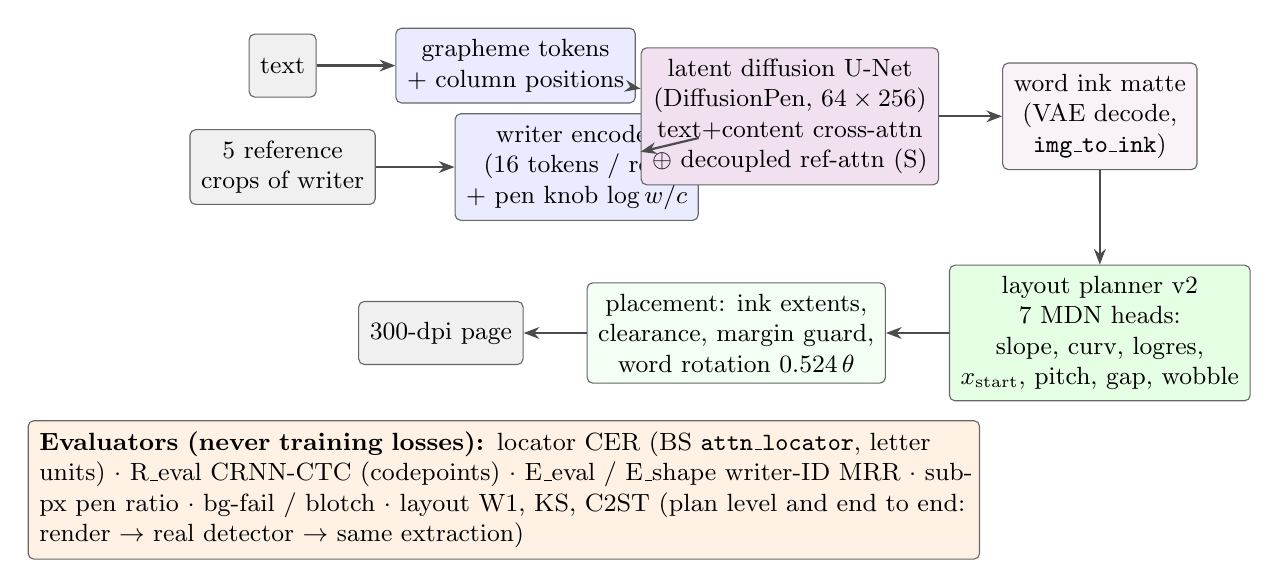
\begin{tikzpicture}[
  font=\small, node distance=4mm and 7mm,
  box/.style={draw=black!60, rounded corners=2pt, fill=#1, align=center, inner sep=4pt, minimum height=8mm},
  box/.default=white, arr/.style={-{Stealth[length=2mm]}, black!70, thick}]
\node[box=gray!12] (text) {text};
\node[box=gray!12, below=of text] (refs) {5 reference\\crops of writer};
\node[box=blue!8, right=10mm of text] (tok) {grapheme tokens\\+ column positions};
\node[box=blue!8, right=10mm of refs] (enc) {writer encoder\\(16 tokens / ref)\\+ pen knob $\log w/c$};
\node[box=violet!12, right=12mm of $(tok)!0.5!(enc)$, minimum width=34mm] (unet) {latent diffusion U-Net\\(DiffusionPen, $64\times256$)\\text+content cross-attn\\$\oplus$ decoupled ref-attn (S)};
\node[box=violet!5, right=8mm of unet] (ink) {word ink matte\\(VAE decode,\\\texttt{img\_to\_ink})};
\node[box=green!10, below=12mm of ink] (plan) {layout planner v2\\7 MDN heads:\\slope, curv, logres,\\$x_\mathrm{start}$, pitch, gap, wobble};
\node[box=green!5, left=8mm of plan] (place) {placement: ink extents,\\clearance, margin guard,\\word rotation $0.524\,\theta$};
\node[box=gray!12, left=8mm of place] (page) {300-dpi page};
\draw[arr] (text) -- (tok); \draw[arr] (refs) -- (enc);
\draw[arr] (tok) -- (unet); \draw[arr] (enc) -- (unet); \draw[arr] (unet) -- (ink);
\draw[arr] (ink) -- (plan); \draw[arr] (plan) -- (place); \draw[arr] (place) -- (page);
\node[box=orange!10, below=7mm of page, xshift=8mm, text width=118mm, align=left] (ev) {\textbf{Evaluators (never training losses):}
locator CER (BS \texttt{attn\_locator}, letter units) $\cdot$ R\_eval CRNN-CTC (codepoints) $\cdot$ E\_eval / E\_shape
writer-ID MRR $\cdot$ sub-px pen ratio $\cdot$ bg-fail / blotch $\cdot$ layout W1, KS, C2ST (plan level and end to end:
render $\to$ real detector $\to$ same extraction)};
\end{tikzpicture}
\caption{The system. Upper row: the word generator (Arm S configuration; Arm P lacks the reference-token attention). Lower
row: the learned layout and its placement rules. Bottom: the evaluators.}
\label{fig:pipeline}
\end{figure}

%=============================================================================
\section{Data and protocol}
\label{sec:data}

\subsection{Data sets}
\begin{table}[H]
\centering
\caption{Data sources. Only BN-HTR and BanglaWriting are used to train word models. hcr/996 is used for layout and as an
evaluation-only showcase (image\_2).}
\label{tab:data}
\small
\begin{tabular}{@{}p{2.6cm}p{2.6cm}p{1.6cm}p{2.0cm}p{6.0cm}@{}}
\toprule
source & word crops & writers & native size & notes \\
\midrule
BN-HTR & 92,380 labelled + filtered (from 108,181) & 149 & median crop h 74\,px, core $\approx$28--30\,px & 93,758 labelled and $\le$16 graphemes, minus 1,378 flagged by \texttt{label\_filter.json}; folder = writer \\
BanglaWriting (BW) & 20,523 & 260 (\texttt{style\_id} = page = person) & median crop h 163\,px, core $\approx$49\,px & one page per writer; manual labels \\
hcr/996 & $\approx$48.7k word pieces & unknown & A4, 300\,dpi, core median 41\,px & 27 texts copied by many writers; 963 usable pages for layout; no writer IDs \\
\bottomrule
\end{tabular}
\src{\fp{scribe_wordgen/PLAN.md} \S1.6, \S2.1; \fp{runs/T0/REPORT.md}; \fp{scribe_layout/report/scribe_layout_report.tex} \S2}
\end{table}

\subsection{Writer-disjoint splits}
Splits are fixed in \fp{data_cache/splits.json}, and a test asserts that no writer appears in two of them (\fp{runs/T0/REPORT.md}):
\begin{itemize}
\item \textbf{BN-HTR:} TEST = \{15, 22, 24, 28, 30, 48, 51, 54, 69, 136\} (5,768 crops); VAL = \{99, 117, 127, 142, 149\};
  TRAIN = the remaining 134 writers. TEST writers are in BS's generator and locator hold-out, so B0 is scored on writers it
  never saw. The VAL writers are in the TRAIN set of BS's style encoder \texttt{ms4}; this was verified, not assumed
  (\fp{PLAN_REVIEW.md} \S0).
\item \textbf{BanglaWriting:} \texttt{style\_id}s hash-sorted (SHA-256) into 220 TRAIN / 15 VAL / 25 TEST.
  \texttt{dp\_words\_b64} (baseline B3) saw all 260 BW writers, so B3 is fair only on BN-HTR.
\item \textbf{hcr/996 (layout):} split \emph{by source text}: 18 train / 4 val / 5 test texts (test texts \{4, 6, 11, 15,
  18\}), giving 614 / 144 / 193 pages. The v1 report claimed test lines are by unseen writers. The v2 review notes that
  writers likely repeat across texts, which cannot be checked without writer IDs (\S\ref{sec:contradictions}).
\end{itemize}

\subsection{The VAL protocol (word generation)}
Unless stated otherwise every word-generation number uses this protocol (\fp{EXPERIMENTS.md}, header):
\begin{itemize}
\item \textbf{20 VAL writers}: the 5 BN-HTR VAL writers plus the 15 BW VAL writers, with \textbf{781 target words} in total.
\item \textbf{5 conditioning references per writer.} For BN-HTR these come from page A and the targets from other pages. For
  BW the refs and targets come from the same (only) page, which inflates BW style metrics through page cues
  (\fp{runs/P1a/REVIEW.md} \S4).
\item Targets whose text is among the refs are excluded. Punctuation-only targets (54/781, all BW) are excluded from the
  headline CER.
\item \textbf{Seeds.} B0 and real have one sample per word. Diffusion arms have two seeds from eval\_v3 onward. Paired
  comparisons merge on (dataset, writer, idx, seed\_k) and never zip lists.
\end{itemize}

\subsection{TEST status}
\textbf{TEST evaluation (Checkpoint C) regenerated on 2026-10-22 06:14--10:13 UTC.} The final TEST evaluation
(Checkpoint C) regenerated S, F1, F8 arms on TEST split (35 writers, 2,756 images per arm) following Phase 1
vocabulary correction. Locator metrics (attn\_locator CER, polygon IoU) computed via regenerated test/\{S,F1,F8\}/
directories; R\_font2real (OCR recognizer) checkpoint was unavailable (Phase 2 training incomplete); pen metrics
computed relative to S (reference) since real images do not carry pen dynamics. Metric CSVs:
\fp{runs/checkpoint\_C/scores/\{S,F1,F8,B0,real\}\_\_s\{0,1\}.csv} (locator);
\fp{runs/checkpoint\_C/rescore\_font2real.csv} (8,268 rows, R\_font2real scores skipped).
FREEZE.json locked with TEST image hashes and Phase 2 recognizer hashes (R\_font0, R\_real, R\_real\_10).
The only TEST contact is that the independent recogniser R\_eval was scored once on real TEST crops (7,665 words,
\S\ref{sec:fonts}). For layout, all design choices were compared on TEST (selection on test). A selection-free VAL
check was run afterwards (\S\ref{sec:layoutval}).

\subsection{Data-handling facts that affect the numbers}
\begin{itemize}
\item \textbf{The BanglaWriting word-crop PNGs are missing from disk.} The files under
  \fp{Diffusion_model_dataset_building/dataset/word_crops/} that \fp{index_bw.csv} points to were deleted. The script
  \fp{wordgen/recog/bw_regen.py} rebuilds the crops in memory from the LabelMe page JSON and JPG in
  \fp{banglawriting/converted/}. It is a faithful port of the original \texttt{parse\_json}/\texttt{crop\_box} and
  label-checks every crop.
\item \textbf{R\_eval BW coverage.} The R\_eval real-crop cache holds \textbf{20,482 of the 20,523} BW words (17,539 TRAIN +
  1,046 VAL + 1,897 TEST rows in \fp{runs/R_eval/cache/bw_*.jsonl}). The 41 missing words are the rows that already failed
  \texttt{measure\_rows} in the T0 data index (\fp{runs/T0/REPORT.md} \S4.2: ok 20,482 of 20,523); the cache's per-split
  counts equal T0's ok-row counts.
\item \textbf{Core-normalised canvas: clip target not met.} The plan's 160-px core-normalised canvas (core 32\,px) clipped
  22.6\% of BN-HTR and 21.1\% of BW TRAIN crops, almost all at the top (\fp{runs/T0/REPORT.md} \S4.3). A writer-prior fallback
  cut this to 18.98\% / 14.57\% (\fp{runs/T0b/REPORT.md}), still far from the $<$1\% target. The SD-VAE round trip also fails
  the plan's IoU gate ($\ge$0.93) at core 32 (image\_2 0.862; \fp{PLAN_REVIEW.md} B1). All generators therefore stayed on
  DiffusionPen's height-normalised $64\times256$ \texttt{fit\_canvas}. The learned layout rescales words by measured core
  anyway.
\end{itemize}

%=============================================================================
\section{Evaluation methodology}
\label{sec:eval}

Every word metric is computed per writer and then averaged over writers. The CI is a writer-level bootstrap: 2,000
resamples, 95\% percentile interval. A ``tie'' means the paired CI includes 0.

\subsection{Locator CER (letter units, per-word mean)}
BS's frozen \texttt{attn\_locator} reads each word on a fixed $64\times256$ canvas. The ink is tight-cropped and
left-aligned; wider words are resized to fit (eval\_v3 truncated B0 words wider than 256\,px, which affects about 10\% of
B0). For target $y_i$ and reading $\hat y_i$,
\begin{equation}
\mathrm{CER}^{\mathrm{loc}}_i=\min\!\Big(1,\ \frac{d_{\mathrm{edit}}(\hat y_i,y_i)}{|y_i|}\Big),\qquad
\mathrm{CER}^{\mathrm{loc}}_w=\frac{1}{|T_w|S}\sum_{i\in T_w}\sum_{s}\mathrm{CER}^{\mathrm{loc}}_{i,s},\qquad
\mathrm{CER}^{\mathrm{loc}}=\frac{1}{20}\sum_w \mathrm{CER}^{\mathrm{loc}}_w .
\end{equation}
The edit distance is in the locator's letter units. The cap at 1 matters: without it, garbage reads of 1-character
punctuation targets gave CERs of 23--29 and 15\% of words had CER $>1$ (\fp{runs/P1a/REVIEW.md} \S1). The locator is
BN-HTR-trained. Its own real-crop CER is 0.056 on BN-HTR VAL and 0.236 on BW VAL (\fp{runs/R_eval/RESULTS.md}), so it
separates arms poorly on BW.

\subsection{R\_eval CER (codepoints, corpus level)}
R\_eval is an independent CRNN-CTC recogniser (\S\ref{sec:fonts}). Its CER is micro-averaged over Unicode codepoints and
not capped:
\begin{equation}
\mathrm{CER}^{R}=\frac{\sum_i d_{\mathrm{edit}}(\hat y_i,y_i)}{\sum_i \max(|y_i|,1)} ,
\end{equation}
where $|\cdot|$ counts codepoints. The CI resamples writers and recomputes the corpus ratio. A paired difference
$\mathrm{CER}^R(a)-\mathrm{CER}^R(b)$ is computed on the same rows (same gold, same writer) and bootstrapped the same way
(\fp{wordgen/recog/metrics.py}). Results are reported for all words and for words of $\ge$3 codepoints. \textbf{Locator CER
and R\_eval CER differ in unit (letters vs codepoints) and in aggregation (capped per-word mean vs corpus ratio). They must
never be compared with each other.}

\subsection{Style: writer-identification MRR (M2, M2s)}
E\_eval and E\_shape are ResNet-18 writer-embedding networks trained with SupCon plus cosine-softmax CE, on TRAIN writers
only. \textbf{E\_eval} sees the normalised ink matte (construction \emph{and} pen). \textbf{E\_shape} sees a spur-pruned
skeleton redrawn at a fixed thin width (construction only). Every source goes through one preprocessing path that ends at
the generators' $64\times256$ canvas (\fp{wordgen/eval/writer_id.py}). For a query word $q$ of writer $w$, each candidate
writer $v$ of the same dataset has a gallery vector $g_v$: the L2-normalised mean embedding of real crops disjoint from
the refs and the query. The galleries are cross-fitted by index parity, and crops with the query's text are removed. With
$r_q$ the rank of $w$ among candidates by $\cos(e_q,g_v)$:
\begin{equation}
\mathrm{MRR}=\frac{1}{20}\sum_w\frac{1}{|Q_w|}\sum_{q\in Q_w}\frac{1}{r_q},\qquad
\mathrm{margin}_q=\cos(e_q,g_w)-\max_{v\ne w}\cos(e_q,g_v).
\end{equation}
Candidates are the VAL writers of the query's own dataset: 5 for BN-HTR (chance MRR 0.457) and 15 for BW (0.221). Pooled
over 20 writers this gives chance top-1 0.10 and chance MRR 0.28. CIs come from a hierarchical bootstrap (writers within
dataset, then queries within writer), paired across methods (\fp{wordgen/eval/style_metric.py}).

\emph{Validity} (\fp{runs/style_eval/tables.md}). Real crops score top-1 0.723 \ci{0.651}{0.786} and MRR 0.821
\ci{0.775}{0.859}. Font renders sit near chance (NotoSans MRR 0.289, Atma 0.268). B0 is far above fonts (B0$-$Noto
$+0.307$ \ci{+0.156}{+0.464}), so the metric sees writer-conditioned shape, not just ``handwriting vs font''.

\subsection{Pen metric (sub-pixel width per core)}
Per word (\fp{wordgen/eval/pen.py}): $M=\{\text{ink}>\mathrm{Otsu}\}$, core $c$ from \texttt{measure\_rows}, skeleton $K$, and
\begin{equation}
w_{\mathrm{sub}}=\frac{\sum_{p:\,\mathrm{ink}_p>0.17}\mathrm{ink}_p}{|K|},\qquad \rho=\frac{w_{\mathrm{sub}}}{c},\qquad
\mathrm{pen}_w=\frac{\operatorname{median}_{i\in\mathrm{gen},w}\rho_i}{\operatorname{median}_{i\in\mathrm{real},w}\rho_i}.
\end{equation}
Ink mass scales with $s^2$ and skeleton length and core with $s$, so $\rho$ is almost resolution-invariant. The reported
value is the median of $\mathrm{pen}_w$ over writers, with p10--p90 and a bootstrap CI of the median. This replaced
eval\_v2's integer EDT width. On a 64-px canvas that metric takes only the values $\{1, 1.83, 3, 3.47,\dots\}$ and
reported 1.8--2.2$\times$ for every generator, where like-for-like measurement gives 1.13--1.36$\times$
(\fp{runs/P1a2/REVIEW.md} \S1).

\subsection{Background metrics}
\textbf{bg-fail}: a word fails when more than 60\% of its ink bounding box is ink, or the box's 25th-percentile ink exceeds
0.1. The rate is a mean of per-writer rates. \textbf{Faint blotch}: a non-punctuation word with $>$2\% of the canvas covered
by faint ink (0.17--0.5) more than 2\,px from strong ink. Writer bnhtr\_117, a grey-paper scanner, is tracked separately.

\subsection{Statistics for claims}
All decisions are made on VAL. A claim of ``A beats B'' needs the paired CI of A$-$B to exclude 0. The paired bootstrap
resamples the same writers (and, for style, the same query positions) for both arms. Each table also gives the count of
writers favouring the first arm.

%=============================================================================
\section{Page layout: v1 to v2}
\label{sec:layout}

\subsection{What is measured}
Layout is learned from real ink geometry on hcr/996. A word detector (the project's \texttt{unified\_cascade} engine: a
Swin-T Mask R-CNN line detector and a word detector on line strips) gives 50-point word polygons. Only the word polygons are
kept, because the line polygons merge on sloped pages. Lines are then rebuilt by chaining words with a robust quadratic fit.
Ink is binarised (Otsu capped at grey 170, components $<$30\,px removed) and assigned to polygons. All geometry is in a
per-page writer unit \textbf{U} = the median word core height (80th minus 20th percentile of ink rows), about 3.5\,mm and
31--54\,px at 300\,dpi. U was chosen because the pitch/U ratio is most stable across writers (CV 0.189).

\paragraph{Real layout statistics (train split; v1 report Table~4).} The real-data statistics shape the model. Gaps
have median 1.14\U{} and lag-1 Spearman 0.49 within a line. Gaps tighten along the line ($-0.13$) and their line mean is a
writer habit (ICC 0.37). Slope is a strong writer habit (ICC 0.77) and persists to the next line ($r=0.87$). Curvature is
weak (ICC 0.17). Pitch has median 4.40\U{} (ICC 0.35). The residual (wobble) scale has median 0.098\U. So spacing and slope
cannot be i.i.d., and the generator must condition on the page's history.

\subsection{The model and its learned parameters}
\label{sec:layoutmodel}
\texttt{LayoutModel} has seven small 1-D mixture-density heads ($k=4$ components, hidden 64), trained by exact NLL with
teacher forcing, full batch, Adam (lr $10^{-3}$, wd $10^{-5}$), patience 30. A page is generated line by line by the chain
rule. For line $k$ with page-history vector $H_k$ (20 running statistics of previous lines):
\begin{multline}
p(\text{line}_k\mid H_k)=p(c_1\mid H)\,p(c_2\mid H,c_1)\,p(\log s\mid H,c_1,c_2)\,p(x_\mathrm{start}\mid\cdot)\,
p(\mathrm{pitch}\mid\cdot)\\ \times\prod_{j}p(\mathrm{gap}_j\mid w_j,w_{j+1},\mathrm{gap}_{<j},\cdot)\prod_j p(r_j\mid \log s,j/n).
\end{multline}
The headline trajectory is $y=c_0+c_1(x-x_m)+c_2(x-x_m)^2$, centred on the line's $x$ midpoint, plus per-word residuals
$r_j$ (``wobble'') with robust scale $s$. Curvature needs $\ge$5 words and slope $\ge$3. The model learns slope, curvature,
residual scale, line start, pitch, gaps (autoregressive) and wobble. v2 adds fitted constants and placement rules.
Table~\ref{tab:layoutparams} lists all of them.

\begin{table}[H]
\centering
\caption{Learned and fitted layout parameters of the final default (v2 \texttt{default\_unfitw\_dc}). All constants are fitted
on the train split.}
\label{tab:layoutparams}
\small
\begin{tabular}{@{}p{4.3cm}p{6.2cm}p{5.2cm}@{}}
\toprule
parameter & value & role \\
\midrule
MDN heads & 7 heads, $k=4$, hidden 64; best epoch 152 (stopped 183) & slope, curv, logres, $x_\mathrm{start}$, pitch, gap, wobble \\
training rows & slope 4,942; curv/logres 4,050; $x_\mathrm{start}$ 4,814; pitch 4,258; gap 25,546; wobble 26,878 & per-head targets \\
val NLL (nats) & slope $-2.363$, curv $-1.004$, logres 1.071, $x_\mathrm{start}$ 0.965, pitch 1.152, gap 0.669, wobble $-0.606$ & \\
combined word anchor & $w=0.349$ headline + $0.651$ median-ink-row & inverse-noise weighting \\
anchor noise & true wobble var 0.00906\U$^2$; noise var headline 0.01176, mid 0.00631, combined 0.00411 & deconvolution of wobble \\
wobble de-noise factor & $\sqrt{1-\text{share}_\text{combined}}\approx0.83$ (share 0.29--0.33) & generation-time scale \\
unfit targets & per-word leverage inflation $1/\sqrt{1-h_i}$, cap 4; line scale keeps the median-MAD table & restores physical wobble \\
curvature deconvolution & noise = 38.4\% of curv target variance; MDN likelihood $\sum_k\pi_k\mathcal N(c;\mu_k,\sigma_k^2+v_i)$ & sampling is noise-free \\
line clearance & min distance $\ge2.603$\U, min/mean $\ge0.797$ (train 1st pct.); 30 redraws, else push down & stops line collisions \\
word rotation & $\beta=0.524\times$ line tangent angle (Huber fit, $n=26{,}653$) & tilts words with the line \\
placement & ink-extent edges (\texttt{INK\_LEVEL} 0.35); planner reset per page; margin guard $\pm0.3$\U & BS integration \\
\bottomrule
\end{tabular}
\src{\fp{scribe_layout_v2/runs/default_unfitw_dc/metrics.json}, \fp{.../default_unfitw_dc/tilt.json},
\fp{scribe_layout_v2/runs/anchor_noise.json}, \fp{.../line_clearance.json}, \fp{scribe_layout_v2/report/FACTS.md} items 1--11}
\end{table}

\subsection{Metrics: W1, KS and C2ST}
Every generator receives each real TEST page's word widths and line breaks. Its plan is converted to raw coordinates and
\emph{re-measured by the same code} that measured the real lines. For each marginal quantity $q$ (gap, slope, curvature,
residual scale, drift $y_n-y_1$, pitch, $x_\mathrm{start}$) we report the Wasserstein-1 distance and the KS statistic
between generated and real distributions:
\begin{equation}
W_1(P,Q)=\int|F_P(t)-F_Q(t)|\,dt,\qquad \mathrm{KS}(P,Q)=\sup_t|F_P(t)-F_Q(t)|.
\end{equation}
The \textbf{classifier two-sample test (C2ST)} trains a classifier (logistic regression unless marked MLP) to tell real
lines (or pages) from generated ones. It uses grouped 5-fold cross-validation, where each real page and its generated copy
form one group, and reports out-of-fold AUC. AUC $=0.5$ means indistinguishable. Line features (lines with $n\ge5$): mean
and sd of gaps, gap lag-1, slope, curvature, residual scale, drift, gap--width correlation. Page features: mean and sd of
line-mean gaps, mean and sd of slope, slope lag-1, mean curvature, mean residual scale, mean pitch.

\emph{Nulls.} The ``shuffled real'' baseline (another page's geometry) is \textbf{not} a floor. It breaks the gap--width
relation, which is a C2ST feature (0.018 vs real 0.130). The comparable null splits each real page into two labels inside
one group: $0.496\pm0.019$. End to end, the floor is real TEST pages split in half: line 0.534, page 0.508.

\subsection{Results in chronological order}

\paragraph{v1 (\fp{scribe_layout/}).} Table~\ref{tab:v1abl} is v1's own ablation on its own harness. The learned model
reduces gap W1 from 0.490 (naive) and 0.559 (manual) to 0.038. Vertical structure (slope, drift, pitch) comes from the
vertical heads, spacing from the gap head; each alone leaves the other at manual's level. The weak point is
$x_\mathrm{start}$ (W1 1.31\U), worse than shuffled real (0.43). Model selection chose $k=4$ (summed val NLL 0.417, against
1.710 for $k=1$; \fp{scribe_layout/runs/model_ablation.json}).

\begin{table}[H]
\centering
\caption{v1 ablation (v1 harness, TEST, 5 seeds, mean $\pm$ sd). W1 is in U.}
\label{tab:v1abl}
\small
\begin{tabular}{@{}lcccccc@{}}
\toprule
method & gap W1 & slope W1 & drift W1 & pitch W1 & $x_\mathrm{start}$ W1 & line C2ST \\
\midrule
naive & 0.490 & 0.038 & 1.217 & 0.849 & 1.811 & 1.000 \\
manual & 0.559 & 0.036 & 1.143 & 1.607 & 1.713 & 0.977 \\
learned (v1) & $\mathbf{0.038\pm0.007}$ & $0.005$ & $0.158\pm0.030$ & $0.092\pm0.015$ & $1.314\pm0.021$ & $0.619\pm0.011$ \\
learned, spacing only & $0.043$ & 0.036 & 1.138 & 1.605 & 1.318 & 0.874 \\
learned, vertical only & 0.561 & 0.005 & 0.159 & 0.085 & 1.713 & 0.944 \\
shuffled real & $0.106\pm0.034$ & 0.006 & 0.187 & 0.194 & $0.434\pm0.104$ & 0.588 \\
\bottomrule
\end{tabular}
\src{\fp{scribe_layout/runs/eval/ablation.md}}
\end{table}

\begin{figure}[H]
\centering
\includegraphics[width=0.48\linewidth]{q_layout_geom.png}
\caption{Extracted geometry on a real page (v1 report): word anchors, fitted line trajectories and residuals.}
\src{\fp{scribe_layout/report/fig/image_103_geom.png}}
\end{figure}

\paragraph{v2 harness and the move to ``unfit'' targets.} v2 (\fp{scribe_layout_v2/}) re-evaluates v1 on a stricter harness
with more C2ST features: there, v1's line C2ST is $0.566\pm0.021$. Table~\ref{tab:v2steps} gives the sequence of v2 models.
The first v2 models (\texttt{v2\_history}, \texttt{v2\_latent}) learned the \emph{fitted} wobble. Fitting a quadratic to
$n$ points shrinks the residuals (``fit shrinkage''), and replaying them adds a second fit at measurement. Training on
inflated (``unfit'') targets lowered the line C2ST from 0.638 to 0.539 (single seed then 5 seeds).

\paragraph{A bug in the unfit targets, and the fix.} A review (M2) found that the inflation table matched the \emph{line}
robust scale but was also applied to every per-word residual. This made per-word wobble overshoot: in a simulation with
i.i.d.\ wobble of sd 0.150, the old table recovers 0.311 at $n=5$, while per-word leverage correction recovers 0.142. The
2-D FFT C2ST had already flagged this. Scaling the drawn wobble moved it from 0.683 ($\times1.0$) to 0.578 ($\times0.5$)
(3 seeds). The leverage fix \texttt{unfitw} gave the best line C2ST, $0.521\pm0.019$.

\paragraph{Curvature deconvolution (the default).} In end-to-end runs the real detector split 89 of 462 drawn v2 lines (19\%),
against 6 of 355 (1.7\%) for manual. At the split points, adjacent words stepped by a median 1.2\U, more than the chainer's
1.0\U{} join threshold. The cause was lines that bow too much. Curvature is sampled before the word count is known, and
fitted $c_2$ on 5--6-word lines is mostly noise (measured sd 0.00129, noise 0.00092, implied true 0.00091). An
extreme-deconvolution likelihood removes this: sampled sag matches real ($|$sag$|>0.5$\U{} on 9.3\% of lines, real 10.8\%,
\texttt{unfitw} 17.5\%), and end-to-end splitting halves to 52/469 (11.1\%). Its C2ST is within noise of \texttt{unfitw}.
\texttt{unfitw\_dc} was chosen for realism, not for C2ST.

\paragraph{A rejected variant.} A Huber-aware per-word correction (\texttt{unfitwh\_dc}) is exact for i.i.d.\ wobble, but was
worse on all three C2STs on both splits (6/6 comparisons). Real wobble is smoother than i.i.d.\ (lag-1 $-0.38$ vs $-0.48$),
so the larger edge inflation overshoots.

\begin{table}[H]
\centering
\caption{Plan-level C2ST AUC by model, TEST (193 pages), 5 seeds, mean $\pm$ sd. Resid-scale W1 is given by words per
line.}
\label{tab:v2steps}
\small
\begin{tabular}{@{}lcccc@{}}
\toprule
model & line C2ST & page C2ST & 2-D FFT C2ST & resid\_scale W1, $n$=5 / 6--7 / 8--10 / 11+ \\
\midrule
manual (BengaliScribe) & 0.980 & 1.0 & 0.99 & -- \\
v1 & $0.566\pm0.021$ & $0.654\pm0.043$ & $0.567\pm0.034$ & .011 / .025 / .055 / .074 \\
v2\_history (1 seed) & 0.638 & 0.752 & -- & -- \\
v2\_history\_unfit (old table) & $0.539\pm0.016$ & $0.660\pm0.004$ & $0.653\pm0.024$ & .039 / .028 / .029 / .058 \\
v2 unfitw (leverage) & $\mathbf{0.521\pm0.019}$ & $\mathbf{0.581\pm0.026}$ & $0.566\pm0.025$ & .009 / .011 / .041 / .062 \\
\textbf{v2 unfitw\_dc (default)} & $0.535\pm0.012$ & $0.590\pm0.024$ & $0.550\pm0.020$ & .007 / .011 / .042 / .061 \\
v2 unfitwh\_dc (Huber, rejected) & $0.544\pm0.012$ & $0.614\pm0.011$ & $0.583\pm0.029$ & .009 / .014 / .043 / .068 \\
shuffled real (not a floor) & $0.584\pm0.016$ & $0.605\pm0.012$ & $0.529\pm0.050$ & .021 / .018 / .054 / .100 \\
within-page null & $0.496\pm0.019$ & -- & -- & -- \\
\bottomrule
\end{tabular}
\src{\fp{scribe_layout_v2/runs/compare_unfitw/compare_5seed.txt}, \fp{compare_5seed_dc.txt}, \fp{compare_5seed_wh_test.txt};
v2\_history row: \fp{scribe_layout_v2/runs/eval/metrics.json}; null and manual: \fp{scribe_layout_v2/report/FACTS.md}}
\end{table}

\paragraph{Selection-free VAL check.}
\label{sec:layoutval}
Every choice above was made on TEST, so the TEST numbers are optimistic. Table~\ref{tab:v2val} repeats the comparison on VAL.
The leverage-family models beat v1 on line and page C2ST on VAL too. The old-table \texttt{unfit} model, which looked better
than v1 on TEST (0.539), is not better on VAL (0.566 vs 0.560): that earlier claim was a selection effect.

\begin{table}[H]
\centering
\caption{Plan-level C2ST on the VAL split (4 texts), 5 seeds.}
\label{tab:v2val}
\small
\begin{tabular}{@{}lcccc@{}}
\toprule
model & line C2ST & page C2ST & FFT C2ST & resid\_scale W1 by $n$ \\
\midrule
v1 & $0.560\pm0.024$ & $0.631\pm0.040$ & $0.531\pm0.033$ & .013 / .025 / .055 / .089 \\
v2 unfit (old table) & $0.566\pm0.028$ & $0.660\pm0.022$ & $0.599\pm0.051$ & .049 / .030 / .024 / .050 \\
v2 unfitw & $0.527\pm0.030$ & $0.575\pm0.039$ & $0.528\pm0.024$ & .012 / .011 / .035 / .072 \\
\textbf{v2 unfitw\_dc (default)} & $0.536\pm0.027$ & $0.593\pm0.031$ & $0.535\pm0.044$ & .011 / .011 / .035 / .069 \\
v2 unfitwh\_dc & $0.551\pm0.022$ & $0.619\pm0.043$ & $0.551\pm0.049$ & -- \\
shuffled real & $0.577\pm0.023$ & $0.597\pm0.030$ & $0.480\pm0.034$ & .016 / .017 / .055 / .089 \\
\bottomrule
\end{tabular}
\src{\fp{scribe_layout_v2/runs/compare_unfitw/compare_5seed_val.txt}, \fp{compare_5seed_wh_val.txt}}
\end{table}

\begin{figure}[H]
\centering
\includegraphics[width=\linewidth]{layout_w1_ks.pdf}
\caption{Plan-level marginals against real TEST on the v2 harness: W1 (top) and KS (bottom). Learned layouts (blue, violet)
match gaps, slope, drift and pitch far better than naive or manual layout. $x_\mathrm{start}$ remains the weakest learned
quantity; shuffled real does better there.}
\src{\fp{scribe_layout_v2/runs/eval/metrics.json} (via \fp{make_figs.py})}
\end{figure}

\begin{figure}[H]
\centering
\includegraphics[width=\linewidth]{layout_c2st.pdf}
\caption{C2ST AUC per model. Left and centre: plan level, TEST (solid) and VAL (light), 5 seeds, $\pm$ sd. ``*'' marks the
default. Right: end-to-end line C2ST, balanced protocol only. The two earliest end-to-end runs used a biased C2ST and are
excluded (see text).}
\src{\fp{scribe_layout_v2/runs/compare_unfitw/compare_5seed*.txt}, \fp{scribe_layout_v2/runs/e2e_*/results.md}}
\end{figure}

\paragraph{End-to-end evaluation.} BengaliScribe renders pages for 5 reference writers $\times$ 2 seeds. The real detector
and the same extraction then measure them, and they are compared with the 193 real TEST pages. Variants: \texttt{manual},
\texttt{v2} and \texttt{v2\_ctx} (conditioned on the writer's own real geometry). \textbf{The first two runs
(\texttt{e2e\_unfit}, \texttt{e2e\_unfit\_ink}) used a biased C2ST.} Pooled out-of-fold AUC with one label per page group put
the real-vs-real ``floor'' at 0.34 (line) and 0.115 (page). Their C2ST values are not comparable with later runs; only their
W1 columns are shown. From \texttt{e2e\_pagereset} onward the C2ST is balanced (folds dealt per label; mean of per-fold
AUCs), with floor 0.534 / 0.508.

\begin{table}[H]
\centering
\caption{End-to-end results (W1 in U; AUC). $^{\ddagger}$Biased C2ST: not comparable. Recovered = extracted words /
drawn words.}
\label{tab:e2e}
\small
\begin{tabular}{@{}llccccccc@{}}
\toprule
run (model) & method & gap & slope & drift & pitch & $x_\mathrm{start}$ & line / page C2ST & recovered \\
\midrule
\multirow{2}{*}{e2e\_unfit (canvas-width)} & v2 & 0.602 & 0.015 & 0.531 & 0.716 & 3.837 & \textcolor{gray}{0.750 / 0.901}$^{\ddagger}$ & 0.969 \\
 & v2\_ctx & 0.381 & 0.013 & 0.427 & 0.924 & 4.416 & \textcolor{gray}{0.595 / 0.901}$^{\ddagger}$ & 0.910 \\
\multirow{2}{*}{e2e\_unfit\_ink (ink extents)} & v2 & 0.471 & 0.016 & 0.503 & 0.712 & 4.037 & \textcolor{gray}{0.667 / 0.840}$^{\ddagger}$ & 0.952 \\
 & v2\_ctx & 0.207 & 0.010 & 0.343 & 1.001 & 4.438 & \textcolor{gray}{0.532 / 0.918}$^{\ddagger}$ & 0.866 \\
\midrule
all balanced runs & manual & 0.685 & 0.035 & 0.965 & 1.839 & 0.948 & 0.905 / 0.999 & 1.004 \\
\multirow{2}{*}{e2e\_pagereset (unfit)} & v2 & 0.404 & 0.013 & 0.396 & 0.670 & 4.065 & 0.684 / 0.834 & 0.965 \\
 & v2\_ctx & 0.267 & 0.017 & 0.558 & 0.770 & 3.783 & 0.619 / 0.889 & 0.926 \\
\multirow{2}{*}{e2e\_unfitw} & v2 & 0.376 & 0.012 & 0.343 & 0.346 & 2.278 & 0.699 / 0.851 & 0.960 \\
 & v2\_ctx & 0.197 & 0.019 & 0.610 & 0.480 & 2.703 & 0.613 / 0.842 & 0.933 \\
\multirow{2}{*}{e2e\_unfitw\_dc} & v2 & 0.387 & 0.021 & 0.645 & 0.465 & 1.453 & 0.719 / 0.844 & 0.983 \\
 & v2\_ctx & 0.183 & 0.023 & 0.695 & 0.535 & 2.494 & 0.654 / 0.847 & 0.929 \\
\multirow{2}{*}{\textbf{e2e\_final} (default + margin guard)} & v2 & 0.425 & 0.021 & 0.672 & 0.390 & 1.239 & 0.719 / 0.850 & 0.981 \\
 & v2\_ctx & 0.198 & 0.020 & 0.621 & 0.503 & 2.130 & 0.619 / 0.845 & 0.940 \\
\bottomrule
\end{tabular}
\src{\fp{scribe_layout_v2/runs/e2e_{unfit,unfit_ink,pagereset,unfitw,unfitw_dc,final}/results.md}}
\end{table}

Reading the end-to-end numbers:
\begin{itemize}
\item \textbf{The planner reset was a real fix.} The history used to run across pages, reaching 56--72 lines against at most
  16 in training. Slopes random-walked to the $-0.2$ clamp and words were drawn past the page bottom. After the reset, page
  slope means stay near the writer's (e.g.\ image\_104 with context: $-0.053\dots-0.009$ against real $-0.023$).
\item \textbf{Slope and drift W1 are not comparable across runs with different split rates} (survivor bias). Split lines
  are the steep and bowed ones. In \texttt{e2e\_unfitw}, kept lines had median $|$slope$|$ 0.026 against 0.046 for split
  lines. All drawn \texttt{dc} lines have median $|$slope$|$ 0.027 (q90 0.071), against real 0.029 (0.086).
\item \textbf{Placement bias.} Ink extents use \texttt{INK\_LEVEL} 0.35 while page Otsu is $\approx$0.39, which leaves a
  $+0.067$\U{} bias in every measured gap.
\item \textbf{Line splitting.} With 57 of 453 drawn lines split (12.6\%) in \texttt{e2e\_final}, end-to-end metrics see
  only the surviving lines, and the large $x_\mathrm{start}$ W1 mostly comes from fragments that start mid-page.
\end{itemize}

\begin{figure}[H]
\centering
\includegraphics[width=\linewidth]{layout_e2e_final_w1.pdf}
\caption{End-to-end W1 to real TEST for the final run (\texttt{e2e\_final}).}
\src{\fp{scribe_layout_v2/runs/e2e_final/results.md}}
\end{figure}

\begin{figure}[H]
\centering
\includegraphics[width=\linewidth]{q_layout_thumbs.png}
\caption{\texttt{e2e\_final} pages for reference writer image\_104 (BengaliScribe B0 words): manual layout (left), v2 (centre),
v2 with writer context (right).}
\src{\fp{scribe_layout_v2/runs/e2e_final/thumbs/image_104_{manual,v2,v2_ctx}.png}}
\end{figure}

\paragraph{Final default model.} \fp{scribe_layout_v2/runs/default_unfitw_dc/model.pt} is the default of
\fp{bscribe_run.py} and \fp{relayout.py}. It runs with the margin guard: a line whose ink would cross the bottom margin starts
a new page and is replanned from scratch. A test asserts that ink stays within the margins $\pm0.5$\U; it fails on the old
code. The layout test suite grew from 32 tests ($\approx$8\,min) to 70 ($\approx$17\,s). The latent writer-style variant is
\textbf{not} the default: a context bug fix (causal-prefix $z$) improved the context case but regressed the no-context model
(page C2ST 0.684 $\to$ 0.829), and the issue is unresolved.

\subsection{Spectral side-studies, with corrections}
\label{sec:spectral}

\paragraph{2-D FFT layout-realism metric (\fp{scribe_layout_fft2d/}).} A layout map is the filled word boxes at 8\,px/U,
Hann-windowed. Its 2-D power spectrum is summarised as radial PSD (32 bins), angular energy (18 bins) and the vertical
line-pitch peak. \textbf{Only the controlled (text-matched) comparison is valid.} The uncontrolled version is confounded:
single non-layout features alone separate real from generated (text-block height AUC 0.985, median word width 0.90--0.93),
so its AUCs of 0.96--1.0 measured text, page fill and glyphs, not layout. In the controlled test every generator runs on each
real page's own word widths, both sides use the same fixed box, and confound AUCs are 0.5 by construction.

\begin{figure}[H]
\centering
\includegraphics[width=0.78\linewidth]{spectral_fft2d_controlled.pdf}
\caption{Controlled 2-D FFT C2ST, single seed. Single-seed AUCs move by up to $\pm0.09$; the 5-seed FFT C2STs are in
Table~\ref{tab:v2steps}. Pitch ablations on real pages show that the spectrum is dominated by line-pitch regularity.
Shuffling pitch moves the mean log-PSD 6$\times$ more (L2 0.080) than zeroing slope (0.013) or removing wobble (0.013).}
\src{\fp{scribe_layout_fft2d/runs/results.md} (controlled section only), \fp{scribe_layout_v2/report/FACTS.md}}
\end{figure}

\begin{figure}[H]
\centering
\includegraphics[width=\linewidth]{q_fft_layout_maps.png}
\caption{Controlled layout maps (fixed word boxes) used by the 2-D FFT metric: real page and generated layouts on the same
word widths.}
\src{\fp{scribe_layout_v2/report/figs/example_layout_maps_fair.png}}
\end{figure}

\paragraph{1-D Fourier model of the headline (\fp{scribe_layout_fourier/}).} Dense headline traces of real lines follow a
power law, PSD $\propto f^{-\alpha}$ with $\alpha=1.06$ ($R^2=0.99$, 5,099 train lines), with no word-period peak. A
spectral-synthesis generator samples Gaussian-process headlines with this spectrum. Its \fp{runs/results.md} states that
Fourier is ``17$\times$ better'' than v1 (log-spectral RMSE 3.98 vs 0.23 nats). \textbf{That claim is wrong.} The 0.23
belongs to a continuous trace that no layout of rigid words can draw. v1's 3.98 is a floor artefact, because the comparison
ran on traces that a layout cannot realise. The corrected, fair comparison uses layout-realisable traces (rigid, rotated
words) and the band with wavelength $\ge$4\U. The distance to real is then: manual 3.786, \textbf{v1 0.702, Fourier 0.668},
continuous Fourier (not realisable) 0.244. \textbf{Fourier and v1 are essentially equal.} The ``6$\times$ better
$x_\mathrm{start}$'' claim from the same study came from including indents.

\begin{figure}[H]
\centering
\includegraphics[width=\linewidth]{spectral_fourier_fair.pdf}
\caption{Corrected Fourier comparison. Left: mean log PSD of dense headline traces (dotted line: the 4\U{} wavelength
limit). Right: log-spectral distance to real in the layout band.}
\src{\fp{scribe_layout_fourier/runs/fair_dense_psd.json}; correction in \fp{scribe_layout_v2/report/FACTS.md}}
\end{figure}

%=============================================================================
\section{Word generation}
\label{sec:wordgen}

\subsection{From diagnosis to design}
The diagnosis (\S\ref{sec:intro}) implies that a higher-resolution B0 would still copy the font: construction has to be
learned from the references by a model that is not tied to a font raster. The primary approach is a \textbf{few-shot latent
diffusion word generator} built from DiffusionPen: an SD-1.5 VAE, a U-Net with CANINE text cross-attention, and a style
vector from 5 references. Candidates are re-adapted from the IAM checkpoint on TRAIN writers only. \texttt{dp\_words\_b64},
which saw every BW writer, is used only as a probe and a baseline (B3). Table~\ref{tab:armlist} lists the arms.

\begin{table}[H]
\centering
\caption{Generator arms.}
\label{tab:armlist}
\small
\begin{tabular}{@{}lp{12.6cm}@{}}
\toprule
arm & definition \\
\midrule
B0 & BengaliScribe font-prior GAN (NotoSans prior), \texttt{models/v2} \\
B3 & \texttt{dp\_words\_b64}: DiffusionPen fine-tuned on all 260 BW writers (fair only on BN-HTR) \\
A, B (P1a) & DiffusionPen from IAM on TRAIN, 40 crops/writer cap, 20k steps; B adds an 8-ch painted grapheme content map \\
\Ap, \Bp{} (P1a$'$) & full TRAIN (98,856 crops, 354 writers), white-paper normalisation, 40k steps; \Bp{} adds grapheme tokens + column-position encodings in cross-attention \\
\Bp{}v2 & \Bp{} sampled with \texttt{fit\_canvas\_white2} (bgnorm2) references, no retraining \\
P & \Bp{} + pen knob (scalar embedding of the refs' $\log$ width/core) + learned null style + rebalanced sampling; 16k steps \\
S & P + 16 reference tokens per ref (Bengali SupCon ResNet-18) in decoupled (IP-Adapter-style) cross-attention; 24k steps \\
\_tXcY / \_cal & text guidance X and content guidance Y; \_cal = page-scale pen calibration (shrink mode) \\
\bottomrule
\end{tabular}
\end{table}

\subsection{probe\_day1: a visible first probe}
\texttt{dp\_words\_b64} was sampled on image\_2's text with three reference sets, and fine-tuned for 120 steps on image\_2's
confident crops. The result was qualitatively the most handwriting-like texture yet: rounder and more flowing than B0
(Fig.~\ref{fig:probe}). But it was not thinner than B0, and it misspelled conjuncts and long words (Table~\ref{tab:probe}).

\begin{table}[H]
\centering
\caption{probe\_day1 (24 image\_2 words; locator CER, mean). Real CER is circular: the ``confident'' crops were selected by
the same locator. Indicative only.}
\label{tab:probe}
\small
\begin{tabular}{@{}lcccc@{}}
\toprule
method & $n$ & width/core (median) & darkness (median) & locator CER \\
\midrule
real (confident crops) & 9 & 0.064 & 1.00 & 0.00 (circular) \\
B0 & 24 & 0.063 & 0.97 & 0.184 \\
DP, image\_2 refs & 24 & 0.091 & 1.00 & 0.973 \\
DP, writer\_99 refs & 24 & 0.110 & 1.00 & 0.931 \\
DP, writer\_117 refs & 24 & 0.104 & 1.00 & 0.899 \\
DP, fine-tuned on image\_2 & 24 & 0.100 & 1.00 & 0.651 \\
\bottomrule
\end{tabular}
\src{\fp{scribe_wordgen/runs/probe_day1/REPORT.md} (``Numbers'')}
\end{table}

\begin{figure}[H]
\centering
\includegraphics[width=\linewidth]{q_probe_line.png}
\caption{probe\_day1: the first line of image\_2, rendered by different methods (real, B0 and DiffusionPen variants).}
\label{fig:probe}
\src{\fp{scribe_wordgen/runs/probe_day1/line.png}}
\end{figure}

\subsection{P1a: the painted content map is inert (NO-GO)}
P1a trained DiffusionPen from IAM on TRAIN writers (40 crops/writer: 14,155 crops, 5,033 unique texts), 20k steps at
batch 32. Arm A is the text-only control; arm B adds an 8-channel grapheme content map with a zero-initialised first-conv
slice. The review first corrected the metric. Raw CER $>1$ and width/core $\approx4$ were artefacts of uncapped CER on
punctuation, grey-box output on grey-paper writer 117, and truncation of B0 at 256\,px. Table~\ref{tab:p1a} gives the
corrected numbers.

\begin{table}[H]
\centering
\caption{P1a, corrected (VAL, 20 writers; CER capped at 1, left-aligned, punctuation excluded).}
\label{tab:p1a}
\small
\begin{tabular}{@{}lccccc@{}}
\toprule
method & CER & BN-HTR excl.\ 117 & BW & bg-fail \% & sub-px width / real \\
\midrule
real & 0.133 \ci{0.101}{0.169} & 0.049 & 0.237 & 1.2 & 1.00 \\
B0 & 0.130 \ci{0.105}{0.157} & 0.084 & 0.224 & 0.2 & $\approx$1.3 \\
B3 & 0.422 \ci{0.384}{0.460} & 0.427 & 0.476 (optimistic) & 3.8 & 1.32 \\
A & 0.482 \ci{0.440}{0.528} & 0.423 & 0.525 & 8.7 & 1.40 \\
B & 0.457 \ci{0.417}{0.501} & 0.361 & 0.516 & 8.8 & 1.40 \\
\bottomrule
\end{tabular}
\par\smallskip\footnotesize Paired B$-$A $=-0.024$ \ci{-0.045}{-0.002} (14/20 writers), entirely in-vocabulary (OOV: A 0.568, B 0.574).
\src{\fp{scribe_wordgen/runs/P1a/REVIEW.md} \S1}
\end{table}

\textbf{Verdict: NO-GO for the content map.} When another word's map is painted in, the model still writes the CANINE word:
CER against the painted word is 0.959. The map alone gives near-unconditional output (0.953 vs 0.973). The grapheme
embeddings barely moved during training (row norm 0.078 vs init $\approx$0.057). One content patch contributes about 2\% of
the first-conv input signal. The review traced the other failures to grey reference paper (6.4\% of BN-HTR TRAIN crops have
paper $<250$), a starved data set, and a CFG-driven thick pen (arm A: 1.31$\times$ at g1, 1.48$\times$ at g2/g3).

\subsection{P1a$'$: full data, white paper, grapheme tokens and the CFG-null bug}
P1a$'$ applied the review's fixes. It trained on all of TRAIN (98,856 crops) for 40k steps with white-paper normalisation,
and redesigned content as \emph{grapheme-token cross-attention}: learned grapheme embeddings plus column-centre and span
encodings, appended to the CANINE context. The report concluded that \Bp{} was a NO-GO (CER 0.550, worse than \Ap). The
review found the cause.

\paragraph{The CFG-null bug.} \texttt{eval\_v2.sample\_arm2} put the content map and tokens into \emph{both} classifier-free
guidance branches. Guidance therefore extrapolated only the text direction, and content was never guided. The correct null
drops text, map and tokens together, matching the independent 10\% drops used in training. With the joint null (same 781
words, refs and seeds; Table~\ref{tab:p1a2}), \Bp{} becomes the best diffusion arm. The shuffled-content gate passes: the
model writes the \emph{painted} word (CER 0.432 against it at g3). Without any text, content alone writes the word at 0.199.
The content-path ablation shows that the tokens carry identity (tokens alone 0.338), while the painted map is still inert
(map alone 0.902).

\begin{table}[H]
\centering
\caption{P1a$'$ on full VAL with the fixed sampler (eval\_v2 scoring; CER capped at 1, punctuation excluded).}
\label{tab:p1a2}
\small
\begin{tabular}{@{}lccccccc@{}}
\toprule
method & CER all & in-vocab & OOV & BN-HTR & BW & bg-fail & pen (sub-px/core) \\
\midrule
real & 0.133 & 0.129 & 0.150 & 0.055 & 0.159 & 1.2\% & 1.00 \\
B0 & 0.130 & 0.116 & 0.235 & 0.085 & 0.145 & 0.2\% & 1.15 \\
B3 & 0.421 & 0.400 & 0.508 & 0.410 & 0.425 & 3.8\% & 1.13 \\
\Ap{} g2 (as reported) & 0.334 & 0.312 & 0.496 & 0.237 & 0.367 & 5.4\% & 1.36 \\
\Ap{} g3 & 0.245 \ci{0.205}{0.287} & 0.228 & 0.384 & 0.160 & 0.273 & 5.2\% & 1.22 \\
\Bp{} as reported (buggy CFG) & 0.550 & 0.537 & 0.655 & 0.405 & 0.599 & 0.9\% & -- \\
\Bp{} fixed g2 & 0.262 \ci{0.218}{0.304} & 0.239 & 0.385 & 0.153 & 0.298 & 1.3\% & 1.27 \\
\textbf{\Bp{} fixed g3} & \textbf{0.188} \ci{0.150}{0.226} & 0.169 & 0.301 & 0.108 & 0.214 & 1.8\% & 1.29 \\
\Bp{} content only, c4 & 0.199 \ci{0.161}{0.238} & 0.186 & 0.303 & 0.112 & 0.229 & 1.7\% & -- \\
\bottomrule
\end{tabular}
\par\smallskip\footnotesize Paired \Bp{}g3$-$\Ap{}g3 $=-0.057$ \ci{-0.089}{-0.032} (18/20 writers). \Ap{} vs P1a A: $-0.147$
\ci{-0.204}{-0.103} (20/20).
\src{\fp{scribe_wordgen/runs/P1a2/REVIEW.md} \S1--2}
\end{table}

\Ap{} and \Bp{} draw about 1.3$\times$ the writer's pen relative to letter size. That is thicker than B0/B3 (about 1.15),
probably because P1a$'$ training is 84\% BN-HTR, whose pens are thick. Writer 117's faint grey blotches (45--48\% of its words)
were not caught by the bg-fail metric, which motivated the faint-blotch score.

\begin{figure}[H]
\centering
\includegraphics[width=0.92\linewidth]{q_compare_image2.png}
\caption{Side-by-side on image\_2 (24 words, seed 0; the real crop exists for 9 words). Columns: real, B0, B3, P1a A,
P1a$'$ \Ap{} g3, \Bp{} g3 (fixed CFG), plain Atma font. The locator's reading and CER are printed under each cell. image\_2
CER over 3 seeds: B0 0.17, B3 0.62, A 0.64, \Ap{} 0.40, \Bp{} 0.34, Atma 0.08; pen vs writer 1.11 / 2.51 / 1.68 / 1.70 /
1.98 / 1.50.}
\src{\fp{scribe_wordgen/runs/compare_inference/image2_side_by_side.png}, \fp{image2_scores.txt}, \fp{README.md}}
\end{figure}

\subsection{eval\_v3: re-baseline and guidance sweep}
eval\_v3 is the corrected evaluation. It uses the fixed joint CFG null and separate text ($t$) and content ($c$) guidance
scales. The decomposition is $\epsilon=\epsilon_{00}+c\,(\epsilon_{0c}-\epsilon_{00})+t\,(\epsilon_{tc}-\epsilon_{0c})$,
where the subscripts mark which conditioning (text, content) is present. eval\_v3 also adds $\ge$2 seeds per word, the
sub-pixel pen metric, a non-punctuation background gate, the faint-blotch score, and OOV CER on all 20 writers. Seed 0
reproduces the review exactly: \Bp{} t3c3 gives 0.188 with 781/781 pixel-identical renders (\fp{runs/eval_v3/validate.txt}).
Raising guidance lowers CER monotonically to t5c5, which ties B0 (Table~\ref{tab:ev3},
Fig.~\ref{fig:guid}). Pen rises slightly with guidance, and the writer-117 blotch rate falls from 34\% (t2c2) to 11\%
(t5c5).

\begin{table}[H]
\centering
\caption{eval\_v3 guidance sweep for \Bp{} (VAL, 2 seeds; locator CER).}
\label{tab:ev3}
\small
\begin{tabular}{@{}lccccccc@{}}
\toprule
method & CER & in-vocab & OOV (18 wr.) & BN-HTR & BW & pen [CI] & blotch 117 \\
\midrule
real & 0.133 \ci{0.100}{0.167} & 0.129 & 0.150 & 0.055 & 0.159 & 1.00 & 8\% \\
B0 & 0.130 \ci{0.103}{0.156} & 0.116 & 0.235 & 0.085 & 0.145 & 1.15 \ci{0.98}{1.20} & 0\% \\
\Ap{} g3 & 0.254 \ci{0.214}{0.295} & 0.234 & 0.379 & 0.161 & 0.285 & 1.22 & 31\% \\
\Bp{} t2c2 & 0.274 \ci{0.229}{0.317} & 0.255 & 0.393 & 0.143 & 0.318 & 1.26 & 34\% \\
\Bp{} t3c3 & 0.194 \ci{0.156}{0.230} & 0.174 & 0.307 & 0.098 & 0.225 & 1.26 & 21\% \\
\Bp{} t4c4 & 0.165 \ci{0.128}{0.202} & 0.151 & 0.254 & 0.077 & 0.194 & 1.27 & 14\% \\
\Bp{} t5c5 & 0.148 \ci{0.115}{0.182} & 0.133 & 0.241 & 0.068 & 0.175 & 1.30 \ci{1.15}{1.45} & 11\% \\
\Bp{} t6c6 & 0.143 \ci{0.110}{0.178} & 0.126 & 0.247 & 0.064 & 0.170 & 1.31 & 11\% \\
\Bp{} t0c4 (content only) & 0.192 & 0.175 & 0.303 & 0.098 & 0.223 & 1.27 & 18\% \\
\bottomrule
\end{tabular}
\par\smallskip\footnotesize Paired: \Bp{}t5c5$-$B0 $+0.018$ \ci{-0.008}{+0.044} (tie); \Bp{}t6c6$-$\Bp{}t5c5 $-0.005$
\ci{-0.011}{+0.000}; OOV \Bp{}t5c5$-$\Ap{}g3 $-0.138$ \ci{-0.218}{-0.066} (14/18 writers).
\src{\fp{scribe_wordgen/runs/eval_v3/report_tables.txt}}
\end{table}

\begin{figure}[H]
\centering
\includegraphics[width=0.95\linewidth]{guidance_sweep.pdf}
\caption{Guidance sweep for \Bp{} with $t=c$. Left: locator CER with writer-bootstrap CI (dashed: real and B0). Right: pen
ratio. More guidance buys legibility, and pen thickens a little.}
\label{fig:guid}
\src{\fp{scribe_wordgen/runs/eval_v3/metrics.json}}
\end{figure}

\subsection{The style evaluator (M2 / M2s)}
Before E\_eval existed, style was judged with the generator's own frozen IAM encoder (real-vs-real MRR 0.41), which is not
independent. E\_eval and E\_shape (\S\ref{sec:eval}) were built and checked before any style claim was made
(Table~\ref{tab:style0}). The first result was sobering: \textbf{every diffusion arm up to \Bp{} sat at MRR 0.40--0.45},
far below B0 (0.596) though above fonts.

\begin{table}[H]
\centering
\caption{Style evaluator validity and early arms (M2, E\_eval, within-dataset galleries, 20 writers / 726 queries).}
\label{tab:style0}
\small
\begin{tabular}{@{}lccc@{}}
\toprule
method & top-1 & MRR & margin \\
\midrule
chance & 0.100 & 0.280 & -- \\
real & 0.723 \ci{0.651}{0.786} & 0.821 \ci{0.775}{0.859} & 0.094 \\
real via \texttt{crop\_ink} & 0.707 & 0.810 & 0.091 \\
B0 & 0.442 \ci{0.310}{0.591} & 0.596 \ci{0.488}{0.711} & $-0.010$ \\
P1a A / P1a B & 0.214 / 0.195 & 0.420 / 0.404 & $-0.133$ / $-0.130$ \\
\Ap{} g3 / \Bp{} g3 & 0.244 / 0.238 & 0.437 / 0.431 & $-0.114$ / $-0.124$ \\
NotoSans font / Atma font & 0.107 / 0.092 & 0.289 / 0.268 & $-0.191$ / $-0.247$ \\
\bottomrule
\end{tabular}
\par\smallskip\footnotesize Paired: real$-$B0 $+0.225$ \ci{+0.116}{+0.335}; \Bp{}g3$-$B0 $-0.165$ \ci{-0.287}{-0.047};
\Bp{}g3$-$Noto $+0.142$ \ci{+0.033}{+0.247}. BN-HTR only: real 0.916, B0 0.883 (real$-$B0 n.s.).
\src{\fp{scribe_wordgen/runs/style_eval/tables.md} (``eval within all'', ``eval within bnhtr'')}
\end{table}

\begin{figure}[H]
\centering
\includegraphics[width=0.78\linewidth]{q_style_prep.png}
\caption{Style-evaluator inputs after the shared preprocessing. Columns: a conditioning reference, the real target, B0,
\Bp{} g3, \Ap{} g3, NotoSans; two variants per row.}
\src{\fp{scribe_wordgen/runs/style_eval/sheet_prep.png}}
\end{figure}

\subsection{Pen calibration (post hoc, no retraining)}
Generation preserves the writer's pen \emph{rank}: Spearman over writers is about 0.9 in pixels. So a per-writer gain is
well posed. \fp{wordgen/pen/calibrate.py} re-renders strokes at page scale toward the refs' measured width.
Table~\ref{tab:pencal} compares the modes on \Bp{} t5c5. All modes bring the pen into $1.0\pm0.1$. The chosen shrink mode
(1.30$\to$1.05) misses the CER gate (upper CI of the CER change $\le+0.01$) by 0.0003. Only the per-writer mode passes both
gates, but its p90 over writers is 2.20.

\begin{table}[H]
\centering
\caption{Pen calibration modes on \Bp{} t5c5 (VAL; pen median over writers, CI of median).}
\label{tab:pencal}
\small
\begin{tabular}{@{}lcccc@{}}
\toprule
mode & pen ratio [CI] & p10--p90 & CER after$-$before & gates (pen / CER) \\
\midrule
before & 1.30 \ci{1.15}{1.45} & 1.06--1.85 & -- & -- \\
writer & 1.09 \ci{0.99}{1.29} & 0.87--2.20 & $+0.0027$ \ci{-0.0030}{+0.0083} & pass / pass \\
writer\_v2 & 1.06 \ci{0.92}{1.21} & 0.80--1.51 & $+0.0049$ \ci{-0.0007}{+0.0101} & pass / fail \\
global\_v2 & 1.07 \ci{1.00}{1.26} & 0.85--1.52 & $+0.0046$ \ci{-0.0011}{+0.0103} & pass / fail \\
word\_v2 & 1.05 \ci{0.92}{1.18} & 0.78--1.53 & $+0.0053$ \ci{-0.0011}{+0.0120} & pass / fail \\
\textbf{shrink\_v2 (adopted)} & 1.05 \ci{0.97}{1.18} & 0.83--1.37 & $+0.0051$ \ci{-0.0000}{+0.0103} & pass / fail by 0.0003 \\
\bottomrule
\end{tabular}
\src{\fp{scribe_wordgen/runs/pen_calib/report_Bp_t5c5_pencal_*.txt}}
\end{table}

\begin{figure}[H]
\centering
\includegraphics[width=0.55\linewidth]{q_pencal_top.png}
\caption{Pen calibration, shrink mode: \Bp{} t5c5 before (left), after (centre) and the writer's real crop (right).}
\src{\fp{scribe_wordgen/runs/pen_calib/sheet_Bp_t5c5_pencal_shrink_v2.png} (top part)}
\end{figure}

\subsection{bgnorm2: background normalisation v2}
The single-scalar whitening (90th-percentile paper $\to$ 255) left writer 117's references with a grey, graded box, which
the model reproduced as texture. \texttt{fit\_canvas\_white2} works on luminance only. It divides by a large-kernel
background estimate and soft-clips the paper to exactly 255, keeping ink darkness linear. On TRAIN crops it changes ink mass
by a median ratio of 0.998. It needs no retraining; the references must be passed through it (Table~\ref{tab:bg2}).

\begin{table}[H]
\centering
\caption{bgnorm2 on \Bp{} g3 (references only, no retraining).}
\label{tab:bg2}
\small
\begin{tabular}{@{}lcccc@{}}
\toprule
method & CER & bg-fail (non-punct) & faint blotch (mean) & blotch, writer 117 \\
\midrule
real & 0.133 \ci{0.100}{0.167} & 0.0\% & 0.4\% & 7.5\% \\
\Bp{} g3, v1 refs & 0.188 \ci{0.150}{0.226} & 0.8\% & 3.7\% & 30.0\% \\
\Bp{} g3, bgnorm2 refs & 0.183 \ci{0.142}{0.226} & 0.3\% & 1.8\% & 0.0\% \\
\bottomrule
\end{tabular}
\par\smallskip\footnotesize Paired CER (v2$-$v1 refs) $-0.0042$ \ci{-0.0170}{+0.0079} (11/20 writers). Writer 117 alone: CER
0.080$\to$0.116, blotch 30\%$\to$0\%.
\src{\fp{scribe_wordgen/runs/bgnorm2/bprime_noretrain.txt}, \fp{measure.txt}}
\end{table}

\begin{figure}[H]
\centering
\includegraphics[width=0.38\linewidth]{q_bgnorm2_117.png}
\caption{Writer bnhtr\_117 (grey-paper scans). Columns: real crop, \Bp{} with v1 refs, \Bp{} with bgnorm2 refs. Each cell is
labelled with blotch (b) and CER (c).}
\src{\fp{scribe_wordgen/runs/bgnorm2/sheet_gen_bnhtr_117.png} (builder \fp{scratch/bgnorm2_gen_sheet.py})}
\end{figure}

\subsection{Arm P and Arm S}
\label{sec:armsPS}
Both arms warm-start from the \Bp{} checkpoint and train on 100,868 TRAIN rows encoded with bgnorm2. Training uses batch 32,
lr $10^{-4}$ (10$\times$ for new modules), 300 warm-up steps and a final lr fraction of 0.1. Dropouts are text, content and
style 0.1 and pen 0.05, and the CFG null drops all of them together. Sampling is rebalanced to punctuation 1.5\%, BW 38\% and
BN-HTR 60.5\%, against a natural mix of 2.0 / 15.4 / 82.6\%. Writers within a dataset are weighted by
clip(median pen / writer pen, 0.5, 2.0), which up-weights thin pens. The two arms differ as follows
(\fp{runs/P1a3/{P,S}/config.json}):
\begin{itemize}
\item \textbf{Pen knob} (both). The input is the refs' median $\log(w_\mathrm{sub}/c)$, z-scored with TRAIN statistics
  ($\mu=-1.835$, $\sigma=0.342$) and embedded sinusoidally. A zero-initialised MLP adds it to the timestep embedding, so the
  knob is a no-op at initialisation.
\item \textbf{Null-style fix} (both). In \Bp{}, dropped style fell back to the TRAIN writer-ID label embedding. P and S instead
  use a learned null style vector.
\item \textbf{Reference tokens} (S only). A Bengali writer encoder (ResNet-18, SupCon on TRAIN) turns each ref into 16
  spatial tokens. With slot embeddings, 5 refs give 80 tokens. They enter every transformer block through decoupled
  attention, $\mathrm{out}=\mathrm{attn}(q,\text{text+content})+\text{keep}\cdot W_\mathrm{ref}\,\mathrm{attn}(q,K_\mathrm{ref},V_\mathrm{ref})$.
  $W_\mathrm{ref}$ starts at zero, which keeps the no-op property. Appending the tokens to the shared context would not: 80
  extra keys change the softmax normalisation even with zero weights.
\end{itemize}
P trained for 16k steps (4,012\,s) and S for 24k steps (2,109\,s; final EMA loss 0.0581).

\paragraph{Two diverged S attempts and the gradient bug.} The first two S runs diverged. Run~1's rolling loss jumped from
$\approx$0.065 to above 0.14 within $\sim$800 steps. Run~2 drifted up from $\approx$0.064 to 0.108 by step 1,050 and was
stopped (Fig.~\ref{fig:curvesdiff}). The cause was a gradient bug. DiffusionPen's
\texttt{CheckpointFunction} re-runs each transformer block during backward. The side-channel attributes (\texttt{n\_ref} and
the keep mask) were reset after the forward pass, so the recomputation was a different function: full-context attention
without the reference branch. S therefore trained on wrong gradients. The fix keeps these attributes set; a test checks
that S's gradient matches a run without checkpointing (\fp{wordgen/models/diffusion3.py},
\fp{tests/test_p1a3.py}). The final S config also adds gradient clipping 1.0 and a 2$\times$ reference-token lr multiplier,
which the diverged configs lack.

\begin{figure}[H]
\centering
\includegraphics[width=\linewidth]{curves_diffusion.pdf}
\caption{Training curves. Left: P1a (capped data) and P1a$'$ (full data). The full-data loss level is higher because the
data are harder and more varied; the curves are not comparable across data sets. Right: P and S fine-tunes from \Bp, and the
two diverged S runs (log scale).}
\label{fig:curvesdiff}
\src{\fp{scribe_wordgen/runs/P1a{,2}/{A,B}/metrics.csv}, \fp{runs/P1a3/{P,S,S_diverged_v1,S_diverged_v2}/metrics.csv}}
\end{figure}

\begin{table}[H]
\centering
\caption{P and S on VAL (locator CER, 2 seeds; background and pen). \_cal = shrink-mode pen calibration.}
\label{tab:ps}
\small
\begin{tabular}{@{}lccccccc@{}}
\toprule
method & CER & 1--2 graph & $>$2 graph & OOV & bg-fail non-punct & blotch 117 & pen raw [CI] \\
\midrule
real & 0.133 \ci{0.100}{0.167} & 0.130 & 0.135 & 0.150 & 0.0\% & 8\% & 1.00 \\
B0 & 0.130 \ci{0.103}{0.156} & 0.115 & 0.143 & 0.235 & 0.0\% & 0\% & 1.15 \ci{0.98}{1.20} \\
\Bp{}v2 t5c5 & 0.151 \ci{0.117}{0.186} & 0.146 & 0.157 & 0.246 & 0.6\% & 1\% & 1.29 \ci{1.18}{1.46} \\
P t3c3 & 0.157 \ci{0.118}{0.198} & 0.185 & 0.128 & 0.226 & 3.0\% & 0\% & 1.13 \ci{1.02}{1.28} \\
\textbf{P t5c5} & 0.132 \ci{0.097}{0.171} & 0.163 & 0.104 & 0.194 & 2.7\% & 0\% & 1.15 \ci{1.01}{1.30} \\
S t3c3 & 0.153 \ci{0.115}{0.189} & 0.192 & 0.118 & 0.216 & 3.6\% & 0\% & 1.12 \ci{1.05}{1.21} \\
\textbf{S t5c5} & 0.137 \ci{0.101}{0.174} & 0.173 & 0.104 & 0.202 & 3.0\% & 0\% & 1.13 \ci{1.07}{1.21} \\
P t5c5\_cal & 0.133 & 0.165 & 0.105 & 0.195 & 2.6\% & 0\% & 1.06 \ci{0.97}{1.15} \\
S t5c5\_cal & 0.138 & 0.175 & 0.103 & 0.209 & 3.1\% & 0\% & 1.06 \ci{0.98}{1.12} \\
\bottomrule
\end{tabular}
\par\smallskip\footnotesize Paired CER: P$-$B0 $+0.002$ \ci{-0.028}{+0.037} (10/20); S$-$B0 $+0.007$ \ci{-0.023}{+0.040}
(10/20); S$-$P $+0.006$ \ci{-0.004}{+0.015}; P$-$\Bp{}v2 $-0.019$ \ci{-0.034}{-0.004} (16/20). OOV S$-$B0 $-0.033$
\ci{-0.088}{+0.016}. \textbf{The 1--2-grapheme column and bg-fail for P/S carry the \texttt{img\_to\_ink} short-word
artefact} (\S\ref{sec:smudge}).
\src{\fp{scribe_wordgen/runs/P1a3/eval/report_tables.txt}}
\end{table}

\begin{table}[H]
\centering
\caption{Style for P and S: M2 (E\_eval) and M2s (E\_shape) MRR, VAL, hierarchical bootstrap.}
\label{tab:psstyle}
\small
\begin{tabular}{@{}lcccc@{}}
\toprule
method & M2 MRR (all) & M2 BN-HTR / BW & M2s MRR (all) & M2s BN-HTR / BW \\
\midrule
real & 0.821 \ci{0.775}{0.859} & 0.916 / 0.789 & 0.768 \ci{0.724}{0.812} & 0.927 / 0.715 \\
B0 & 0.596 \ci{0.488}{0.711} & 0.883 / 0.500 & 0.533 \ci{0.453}{0.617} & 0.841 / 0.430 \\
\Bp{}v2 t5c5 & 0.418 \ci{0.355}{0.483} & 0.566 / 0.369 & 0.399 \ci{0.351}{0.449} & 0.609 / 0.330 \\
P t5c5 & 0.443 \ci{0.379}{0.505} & 0.556 / 0.405 & 0.416 \ci{0.367}{0.469} & 0.596 / 0.357 \\
\textbf{S t5c5} & \textbf{0.579} \ci{0.521}{0.635} & 0.745 / 0.523 & \textbf{0.517} \ci{0.469}{0.564} & 0.726 / 0.448 \\
S t5c5\_cal & 0.562 \ci{0.511}{0.615} & 0.716 / 0.511 & 0.518 \ci{0.471}{0.566} & 0.729 / 0.447 \\
\bottomrule
\end{tabular}
\par\smallskip\footnotesize Paired M2: S$-$B0 $-0.017$ \ci{-0.116}{+0.088} ($p=0.72$, 9/20); S$-$P $+0.136$
\ci{+0.085}{+0.187} (17/20); P$-$B0 $-0.153$ \ci{-0.261}{-0.048}. M2s: S$-$P $+0.101$ \ci{+0.057}{+0.140}; S$-$B0 $-0.015$
\ci{-0.091}{+0.061}. Chance: all 0.28; BN-HTR 0.457; BW 0.221.
\src{\fp{scribe_wordgen/runs/P1a3/eval/report_tables.txt}, \fp{runs/P1a3/eval/metrics.json}}
\end{table}

\begin{table}[H]
\centering
\caption{Style for S vs.\ B0 on TEST: M2 (E\_eval) and M2s (E\_shape) MRR, hierarchical bootstrap, within-dataset galleries.}
\label{tab:stylestest}
\small
\begin{tabular}{@{}lcccc@{}}
\toprule
method & M2 MRR (all) & M2 BN-HTR / BW & M2s MRR (all) & M2s BN-HTR / BW \\
\midrule
real & 0.791 \ci{0.747}{0.834} & 0.869 / 0.759 & 0.765 \ci{0.715}{0.809} & 0.845 / 0.733 \\
B0 & 0.562 \ci{0.490}{0.636} & 0.787 / 0.472 & 0.469 \ci{0.411}{0.530} & 0.742 / 0.360 \\
\textbf{S} & \textbf{0.526 \ci{0.467}{0.581}} & 0.593 / 0.500 & \textbf{0.448 \ci{0.405}{0.488}} & 0.534 / 0.413 \\
\bottomrule
\end{tabular}
\par\smallskip\footnotesize Paired M2: S$-$B0 $-0.035$ \ci{-0.108}{+0.038} ($p=0.35$, 17/35); M2s: S$-$B0 $-0.022$
\ci{-0.078}{+0.034} ($p=0.44$, 12/35); Chance (M2, all): 0.193. \textbf{Confirms the VAL tie}: S neither beats nor loses to
B0 on style, on held-out TEST data.
\src{\fp{runs/checkpoint\_C/report\_S\_vs\_B0\_test.json}, \fp{runs/checkpoint\_C/style\_m2\_table\_test.tex}}
\end{table}

All P/S variants pass the planned gates from the P1a$'$ review: CER $\le$ B0+0.05 = 0.180, calibrated pen $\le$1.15, and
writer-117 blotch $<$10\%.

\begin{figure}[H]
\centering
\includegraphics[width=0.95\linewidth]{cer_locator_arms.pdf}
\caption{Locator CER per arm (letter units; capped per-word mean). From \Bp{} t5c5 on, every diffusion arm ties B0 on this
metric.}
\src{\fp{runs/eval_v3/metrics.json}, \fp{runs/P1a3/eval/metrics.json}}
\end{figure}

\begin{figure}[H]
\centering
\includegraphics[width=0.95\linewidth]{style_mrr_arms.pdf}
\caption{Style MRR per arm, with the chance line (dotted) and the real-crop level (dashed, left). The reference tokens of S
lift style from the 0.42--0.44 plateau of \Bp/P to B0's level.}
\src{\fp{runs/P1a3/eval/metrics.json}}
\end{figure}

\begin{figure}[H]
\centering
\includegraphics[width=0.85\linewidth]{pen_ratio.pdf}
\caption{Pen ratio, raw and calibrated (median over 20 writers, 95\% CI of the median).}
\src{\fp{runs/P1a3/eval/metrics.json}}
\end{figure}

\paragraph{Pen-knob sweep.} The knob was multiplied by 0.6--1.6 (g5, seed 0, 8 words $\times$ 20 writers;
Fig.~\ref{fig:knob}). In P the within-writer slope $d\log(\text{generated})/d\log(\text{knob})$ is 0.11 \ci{0.08}{0.14}: the knob
works but is weak. In S it is 0.03 \ci{0.00}{0.05}, \textbf{nearly inert}. The reference tokens apparently carry the pen and
override the scalar. Across writers without a sweep, generated width tracks the knob with slope 0.15 in both arms (Spearman
0.31 P, 0.15 S).

\begin{figure}[H]
\centering
\includegraphics[width=0.92\linewidth]{pen_knob_sweep.pdf}
\caption{Pen-knob sweep. Thin lines: per-writer medians; bold: median over writers. Titles give the within-writer slope with its
95\% CI over writers.}
\label{fig:knob}
\src{\fp{runs/P1a3/eval/sweep.csv}, \fp{runs/P1a3/eval/metrics.json} (\texttt{knob\_sweep})}
\end{figure}

\begin{figure}[H]
\centering
\includegraphics[width=0.9\linewidth]{q_p1a3_sheet_val_top.png}
\caption{VAL words (top of the P1a3 sheet; seed 0). Columns: real, B0, \Bp{}v2 t5c5, P t5c5, S t5c5, P calibrated, S
calibrated. ``refs (bgnorm2)'' rows show the writer's conditioning crops.}
\src{\fp{scribe_wordgen/runs/P1a3/eval/sheet_val.png}}
\end{figure}

\subsection{Page sheets and the smudge fix}
\label{sec:smudge}
Full pages were rendered with the learned layout (\fp{scribe_layout_v2/runs/default_unfitw_dc/model.pt}) for B0, \Bp, P and S.
The writers were image\_2 and three VAL writers (\fp{runs/page_sheets/}). Two problems are visible
(Fig.~\ref{fig:pages}). Generated text on BanglaWriting pages renders smaller than the real page, and P draws dash words
(``--'') as thick bars.

\paragraph{The ``smudges'' were not the model.} Isolated glyphs such as \bnt{০}, \bnt{ও} and \bnt{২} came out as dark
smudges. The cause is in \texttt{img\_to\_ink}. Its 5th-percentile ink floor assumes ink covers $\ge$5\% of the canvas. A
lone glyph covers 2--3\%, so the floor lands on paper texture and a ripple of about 12 grey levels is stretched to black.
The fix \texttt{img\_to\_ink(..., min\_span=100)} keeps the floor at least 100 grey levels below paper. It brings the
lone-glyph ink fraction from 39--56\% down to 2--3\% and leaves normal words unchanged. The fix is opt-in. \textbf{The eval
caches still use the legacy conversion}, so short-word CER and blotch for the diffusion arms P, \Bp{} and S carry the
artefact until all arms are rescored together. The old inks are kept in \fp{runs/page_sheets/cache_v1_smudged/}.

\begin{figure}[H]
\centering
\includegraphics[width=\linewidth]{q_pagesheet_image_2.png}
\caption{Page sheet for image\_2, split into two rows of six panels. Row 1: real page, B0, \Bp{} g5, \Bp{} g3, P g5, P g5
calibrated. Row 2: P g3, P g3 calibrated, S g5, S g5 calibrated, S g3, S g3 calibrated.}
\label{fig:pages}
\src{\fp{scribe_wordgen/runs/page_sheets/sheets/image_2_sheet_l0.png}}
\end{figure}

\begin{figure}[H]
\centering
\includegraphics[width=\linewidth]{q_pagesheet_bw_101_21_0.png}
\caption{Page sheet for BanglaWriting VAL writer bw\_101\_21\_0 (same panel order). The generated text is smaller than the
real writer's.}
\src{\fp{scribe_wordgen/runs/page_sheets/sheets/bw_101_21_0_sheet_l0.png}}
\end{figure}

\begin{figure}[H]
\centering
\includegraphics[width=0.62\linewidth]{q_pagezoom_image_2_top.png}
\caption{Zoom on the first lines of the image\_2 page: B0, then \Bp{} g5, \Bp{} g3, P g5 and P g5 calibrated.}
\src{\fp{scribe_wordgen/runs/page_sheets/sheets/image_2_zoom_l0.png} (top part)}
\end{figure}

\subsection{The BW scale diagnosis and the dash-word fix (page\_sheets\_v2)}
\label{sec:pagesheetsv2}

Next-steps item~7 asked to fix the two page-integration bugs named just above. \textbf{Both are now fixed}, entirely at the
integration layer (\fp{wordgen/integrate/page_sheets.py}; \fp{scribe_layout_v2}, \fp{BengaliScribe-*} and
\fp{wordgen/eval} were not touched), rebuilt into \fp{runs/page_sheets_v2/}.

\paragraph{BW scale diagnosis.} The real BanglaWriting page photo (\fp{banglawriting/converted/<writer>.jpg}) is a tight
crop around the written text at a few hundred pixels (e.g.\ \fp{10_20_0.jpg} is $1328{\times}910$), while every
\emph{generated} page is a full A4 canvas at 300\,dpi ($2480{\times}3508$) with \texttt{FILL\_PAGE=False}, so the writing
starts near the top and most of the page stays blank below it. The old \texttt{build\_page\_sheet()} resized each column's
\emph{whole page} independently to the same display height -- which compares ``real content height'' against ``A4 sheet
height'', not real word size against generated word size. Measuring the median word-polygon height as a fraction of each
image's own height makes the resulting distortion explicit:

\begin{table}[H]
\centering
\caption{page\_sheets\_v2: word-height-as-fraction-of-page-height, before the fix. image\_2's real page is already a
full-resolution A4 scan, so the old comparison happened to be fair there; BW's real photos are not.}
\label{tab:pagescale}
\small
\begin{tabular}{@{}lccc@{}}
\toprule
writer & real word-h / page-h & generated word-h / page-h (P\_t5c5) & ratio \\
\midrule
bw\_10\_20\_0 & $80/910=0.0879$ & $101/3508=0.0288$ & \textbf{3.05$\times$} \\
bw\_101\_21\_0 & $76.7/1129=0.0680$ & $102/3508=0.0291$ & \textbf{2.34$\times$} \\
image\_2 (control) & $95/3513=0.0270$ & $96.5/3508=0.0275$ & $0.98\times$ (already correct) \\
\bottomrule
\end{tabular}
\src{\fp{runs/page_sheets_v2/RESULTS.md} \S1, \fp{measurements.json}}
\end{table}

This is a \emph{display-time} bug, not a generation-time one: the per-word generated pixel height is already close to the
real photo's in absolute terms (97--110\,px vs 77--80\,px, i.e.\ 0.75--0.85$\times$); it only reads 2--3$\times$ too small
because the generated page's own canvas is far taller than the real photo's, mostly empty.

\paragraph{BW scale fix.} New helpers \texttt{\_real\_word\_height\_px()} / \texttt{\_gen\_word\_height\_px()} measure each
column's own median word-polygon height in its native pixel scale. \texttt{build\_page\_sheet()} now, when both
measurements are available: (1)~scales each \emph{generated} column so its word height equals the real page's own
measured word height (the real column stays at native resolution); (2)~crops each generated column to its content
bounding box first, since the real photo is already a tight crop and the mostly-blank A4 margin is not part of what is
being compared; (3)~applies \emph{one shared zoom} to every column (not an independent per-column resize, which would
silently undo the match from steps 1--2) to fit the sheet for display. It falls back to the old behaviour whenever a
measurement is missing (BN-HTR has no real page at all, so it is unaffected). One honest side effect, visible in
Fig.~\ref{fig:pagescalefix}: the fixed BW columns are now noticeably \emph{taller} relative to their own content than the
real photo -- the learned layout model's line pitch relative to word size is wider than this writer's real spacing, and
this fix does not touch line pitch, so the difference is now shown rather than hidden by shrinking the words again.

\begin{figure}[H]
\centering
\includegraphics[width=\linewidth]{page_sheets_v2_compare_10_20_0.png}
\caption{bw\_10\_20\_0, before (\fp{runs/page_sheets}, top) vs after (\fp{runs/page_sheets_v2}, bottom) the scale fix, real
page plus the first three generated columns (B0, \Bp{} g5, \Bp{} g3), cropped from the full sheet for legibility. Per-word
VAL CER / pen / style MRR captions are unchanged by this fix.}
\label{fig:pagescalefix}
\src{\fp{runs/page_sheets_v2/compare_bw_10_20_0.png}}
\end{figure}

\begin{figure}[H]
\centering
\includegraphics[width=\linewidth]{page_sheets_v2_compare_101_21_0.png}
\caption{bw\_101\_21\_0, same before/after crop as Fig.~\ref{fig:pagescalefix} (B0, \Bp{} g5, \Bp{} g3).}
\label{fig:pagescalefix2}
\src{\fp{runs/page_sheets_v2/compare_bw_101_21_0.png}}
\end{figure}

\paragraph{Dash-word fix.} Among the 4 default writers, only \fp{bw\_10\_20\_0} has dash-only ``words'' (two instances of
\texttt{"-"}). Every arm drew these as a thick solid blob instead of a thin dash (B0: ink bbox $185{\times}54$\,px, 24.3\%
of the $64{\times}190$ canvas filled; P\_t5c5: $78{\times}21$\,px, 8.5\% filled) -- BanglaWriting has almost no pure-dash
training crops, so no arm ever learned the stroke shape, the same reason the project's \texttt{is\_punct\_only} filter
already excludes punctuation-only labels from pen targets. The fix, \texttt{is\_dash\_word()} + \texttt{synth\_dash\_ink()},
draws one straight pen stroke directly (no model), thickness set from the writer's own measured pen width off its
already-cached ink (\texttt{pen\_from\_cache}), length $\approx1.15\times$ the writer's core height per dash character.
\texttt{stage\_generate()} now routes dash-word indices through this helper and skips the GPU sampler for them entirely, so
future live GPU runs get the fix for free at zero extra GPU cost. Verified: the fixed dash's rendered polygon height is
$\approx$12\,px, against $\approx$54\,px before -- a thin stroke, not a block, confirmed visually on the rendered page.

\paragraph{Status.} Both bugs are fixed and next-steps item~7 is \textbf{done}. One gap remains, explicitly out of scope
here: the learned layout model's line pitch relative to word size on BanglaWriting pages is unchanged by this fix and
still differs from real writers' spacing (Fig.~\ref{fig:pagescalefix}, ``after''); that line-spacing gap lives in
\fp{scribe_layout_v2} (\S\ref{sec:layout}), not in the page-integration layer this fix touched.

%=============================================================================
\section{GlyphScribe fonts and the R\_eval recogniser}
\label{sec:fonts}

\subsection{Fonts}
The first font search scored 11 Google OFL Bengali fonts against image\_2 (12 hand-verified words) by skeleton chamfer.
Atma, Hind Siliguri and Noto Serif Bengali came out closest, with overlapping CIs; NotoSans ranked 11th of 12
(\fp{runs/font_search/REPORT.md}). Then 37 handwriting fonts, 1 printed font and 4 paper backgrounds were copied from the
public GlyphScribe repository. Its licence covers the code only and the font licences are unknown, so these fonts are for
internal research only. All 38 are Unicode Bengali with correct GSUB shaping. On shape, Atma variants rank first (chamfer
0.162--0.164) and NotoSans ranks 28th of 39. The top $\sim$10 fonts overlap within their CIs (Fig.~\ref{fig:fonts}). Thin
fonts match the pen far better: the writer's width/core is 0.075, against 0.094 for Junudullah Zami and Tagore, 0.068 for
Qayyum Thin and 0.11--0.23 for the Google fonts. No font draws the writer's broken matra.

\begin{figure}[H]
\centering
\includegraphics[width=0.92\linewidth]{fonts_glyphscribe.pdf}
\caption{All scored fonts against image\_2: skeleton chamfer with 95\% CI over 12 words (left), stroke width/core (right).
Blue: NotoSans (BS's font). Red: the printed font.}
\label{fig:fonts}
\src{\fp{scribe_wordgen/runs/font_search/glyphscribe/scores.csv}}
\end{figure}

\begin{figure}[H]
\centering
\includegraphics[width=\linewidth]{q_glyphscribe_sheet.png}
\caption{image\_2's real words (left block) against the closest fonts, each shown raw and pen-matched.}
\src{\fp{scribe_wordgen/runs/font_search/glyphscribe/sheet.png}}
\end{figure}

\subsection{R\_eval: an independent recogniser}
R\_eval answers two questions. Does pretraining on synthetic renders from the 48 fonts (37 GlyphScribe + 11 Google) help
on real handwriting? And how legible are the generator arms to a recogniser the generators never saw? The model is a
\textbf{CRNN-CTC} with 4.94\,M parameters. The input is a $64\times256$ left-aligned ink matte. A conv/ResNet stack reduces it
to $1\times64$, followed by a 2-layer BiLSTM (256 hidden) and 219 classes including blank and unk; decoding is greedy CTC
(\fp{wordgen/recog/model.py}). Synthetic words come from a 203,371-word vocabulary
(\fp{runs/R_eval/vocab_synth.tsv}). They are rendered with HarfBuzz shaping, decorative fonts are down-weighted to
0.3$\times$, and the renders are augmented for thickness, shear, rotation, baseline wave, blur, noise, paper texture and
JPEG. The real data are the 100,868 TRAIN crops. Before launch, a review fixed three blockers: wrong word pairing in
rescoring, double \texttt{crop\_ink} on cached mattes, and an augmentation roll that cut word edges. The whole chain took
1\,h\,50\,min (\fp{runs/R_eval/full_chain.log}).

\begin{table}[H]
\centering
\caption{R\_eval arms and VAL CER (codepoint, corpus; both datasets, 4,299 words; writer-bootstrap CI).}
\label{tab:reval}
\small
\begin{tabular}{@{}lllccc@{}}
\toprule
model & init & data, steps & VAL CER & BN-HTR & BW \\
\midrule
R\_font0 & -- & synthetic only, 60k & 0.4563 \ci{0.3265}{0.5338} & 0.4827 & 0.3538 \\
R\_real & -- & real TRAIN, 30k & 0.0370 \ci{0.0281}{0.0511} & 0.0308 & 0.0614 \\
\textbf{R\_font2real} & R\_font0 & real TRAIN, 30k & \textbf{0.0329} \ci{0.0245}{0.0443} & 0.0283 & 0.0507 \\
R\_mix & R\_font0 & 75\% real + 25\% synth, 30k & 0.0370 \ci{0.0267}{0.0486} & 0.0333 & 0.0514 \\
R\_real\_10 & -- & 10\% of TRAIN writers, 6k & 0.1781 \ci{0.1404}{0.2082} & 0.1731 & 0.1976 \\
R\_font2real\_10 & R\_font0 & 10\% of TRAIN writers, 6k & 0.1147 \ci{0.0797}{0.1366} & 0.1162 & 0.1090 \\
\bottomrule
\end{tabular}
\par\smallskip\footnotesize Batch 128, lr $3\times10^{-4}$, warm-up 500. R\_font2real is selected as R\_eval. For reference, the
locator's letter-unit real-crop CER is 0.056 (BN-HTR VAL) and 0.236 (BW VAL); it is not comparable.
\src{\fp{scribe_wordgen/runs/R_eval/RESULTS.md}, \fp{selection.json}, \fp{R_*/train.log}}
\end{table}

\begin{figure}[H]
\centering
\includegraphics[width=\linewidth]{reval_models_val.pdf}
\caption{VAL CER per recogniser, by dataset (95\% writer-bootstrap CI).}
\src{\fp{runs/R_eval/RESULTS.md}}
\end{figure}

\begin{figure}[H]
\centering
\includegraphics[width=0.85\linewidth]{reval_font_gain_forest.pdf}
\caption{Font-pretraining gain, as paired differences on the same VAL words. It is significant everywhere: small with all
writers, large with 10\% of the writers.}
\src{\fp{runs/R_eval/RESULTS.md} (paired font-pretraining gain table)}
\end{figure}

\paragraph{Findings.} Fonts alone do not transfer (0.456). As a prior they help: $-0.0042$ \ci{-0.0080}{-0.0022} overall
and $-0.0107$ \ci{-0.0167}{-0.0037} on BW with all writers. With 10\% of the writers the gain is $-0.0634$
\ci{-0.0804}{-0.0538}, from 0.178 to 0.115. Mixing synthetic data into fine-tuning (R\_mix 0.0370) does not beat plain
fine-tuning. The remaining errors are mostly lone punctuation (\bnt{,} \bnt{।} \bnt{'}) and Latin/Bengali digit confusion
(Fig.~\ref{fig:errs}).

\paragraph{OOV and TEST.} \textbf{TEST was scored once}, for R\_real and the selected model: 7,665 words.
Overall CER is 0.0429 \ci{0.0293}{0.0606} for R\_real and 0.0342 \ci{0.0228}{0.0492} for R\_font2real. On ``clean'' OOV words
(not in TRAIN and not in the synthetic vocabulary, 237 words) the two give 0.0956 and 0.0854, with overlapping CIs
(Fig.~\ref{fig:oov}). These are two separate estimates; no paired TEST difference was computed.

\begin{figure}[H]
\centering
\includegraphics[width=0.9\linewidth]{reval_oov.pdf}
\caption{In-vocabulary vs OOV CER (overall). ``In synth'' means the word is in the synthetic vocabulary. TEST was scored once.}
\label{fig:oov}
\src{\fp{runs/R_eval/RESULTS.md}}
\end{figure}

\begin{figure}[H]
\centering
\includegraphics[width=0.95\linewidth]{curves_reval.pdf}
\caption{R learning curves. Left: CTC training loss. Right: CER on a 1,024-word VAL sample logged every 1,000 steps. This
in-training estimate is not the full-VAL number of Table~\ref{tab:reval}.}
\src{\fp{runs/R_eval/R_*/train.log}}
\end{figure}

\begin{figure}[H]
\centering
\begin{subfigure}[t]{0.50\linewidth}\centering\includegraphics[width=\linewidth]{q_errors_font2real_val.png}
\caption{R\_font2real, VAL: top error rows.}\end{subfigure}\hfill
\begin{subfigure}[t]{0.40\linewidth}\centering\includegraphics[width=\linewidth]{q_synth_sheet_top.png}
\caption{Synthetic training renders (top of sheet).}\end{subfigure}
\caption{R\_eval errors and synthetic data. Most residual errors are single punctuation marks and digit-script confusions
(19 read as \bnt{১৯}).}
\label{fig:errs}
\src{\fp{runs/R_eval/errors_R_font2real_val.png}, \fp{runs/R_eval/synth_sheet.png}}
\end{figure}

\subsection{Rescoring the generator arms with R\_eval}
\label{sec:rescore}
The cached eval\_v3/P1a3 renders were rescored. They are ink mattes, so they are loaded as $1-\mathrm{png}/255$ with no
re-stretch. Rows are merged on (dataset, writer, idx) against B0 and real, and on (dataset, writer, idx, seed\_k) between
diffusion arms. B0 words wider than 256\,px (about 10\%) are squashed to fit, whereas the locator truncated them.

\begin{table}[H]
\centering
\caption{Generator arms scored by R\_eval (R\_font2real), VAL, codepoint corpus CER.}
\label{tab:rescore}
\small
\begin{tabular}{@{}lcccc@{}}
\toprule
method & $n$ (all) & CER all words & $n$ ($\ge$3cp) & CER $\ge$3 codepoints \\
\midrule
real & 781 & 0.0438 \ci{0.0310}{0.0586} & 666 & 0.0424 \ci{0.0294}{0.0568} \\
B0 & 781 & 0.0302 \ci{0.0248}{0.0358} & 666 & 0.0226 \ci{0.0162}{0.0287} \\
\Bp{} t5c5 (v1 refs) & 1562 & 0.1395 \ci{0.1117}{0.1713} & 1332 & 0.1021 \ci{0.0810}{0.1264} \\
\Bp{}v2 t5c5$^{\ast}$ & 1562 & 0.1412 \ci{0.1125}{0.1749} & 1332 & 0.1024 \ci{0.0823}{0.1272} \\
P t5c5 & 1562 & 0.0905 \ci{0.0664}{0.1179} & 1332 & 0.0577 \ci{0.0402}{0.0786} \\
S t3c3 & 1562 & 0.1084 \ci{0.0804}{0.1408} & 1332 & 0.0678 \ci{0.0501}{0.0888} \\
\textbf{S t5c5} & 1562 & 0.0889 \ci{0.0652}{0.1153} & 1332 & 0.0552 \ci{0.0381}{0.0753} \\
\midrule
\multicolumn{5}{@{}l}{\emph{paired differences} (all words; $\ge$3cp)} \\
S$-$B0 & \multicolumn{2}{c}{$+0.0587$ \ci{+0.0361}{+0.0833}} & \multicolumn{2}{c}{$+0.0326$ \ci{+0.0145}{+0.0523}} \\
S$-$P & \multicolumn{2}{c}{$-0.0016$ \ci{-0.0111}{+0.0076}} & \multicolumn{2}{c}{$-0.0025$ \ci{-0.0099}{+0.0050}} \\
P$-$B0 & \multicolumn{2}{c}{$+0.0603$ \ci{+0.0375}{+0.0860}} & \multicolumn{2}{c}{$+0.0351$ \ci{+0.0174}{+0.0567}} \\
B0$-$real & \multicolumn{2}{c}{$-0.0136$ \ci{-0.0268}{-0.0021}} & \multicolumn{2}{c}{$-0.0198$ \ci{-0.0347}{-0.0067}} \\
\bottomrule
\end{tabular}
\par\smallskip\footnotesize $^{\ast}$\Bp{}v2 is not in \fp{RESULTS.md}; its row is from the full rescoring table in \fp{runs/R_eval/full_chain.log}.
\src{\fp{scribe_wordgen/runs/R_eval/RESULTS.md} (``scored with R\_eval''), \fp{runs/R_eval/rescore.csv}}
\end{table}

\begin{figure}[H]
\centering
\includegraphics[width=0.88\linewidth]{reval_arms.pdf}
\caption{R\_eval CER per arm. Solid: all words. Light: words of $\ge$3 codepoints. The large drop from all words to $\ge$3cp
for P and S is partly the short-word \texttt{img\_to\_ink} artefact.}
\src{\fp{runs/R_eval/RESULTS.md}}
\end{figure}

\begin{figure}[H]
\centering
\includegraphics[width=\linewidth]{forest_paired.pdf}
\caption{Paired differences S$-$B0, S$-$P and P$-$B0, with 95\% writer-bootstrap CIs, for CER (top) and style (bottom). The
locator cannot separate the arms. R\_eval shows S and P less legible than B0 and tied with each other. Style shows S tied with
B0 and clearly better than P. \emph{The CER panels are in different units.}}
\src{\fp{runs/P1a3/eval/metrics.json}, \fp{runs/R_eval/RESULTS.md}}
\end{figure}

\paragraph{How to read the legibility gap.}
\begin{itemize}
\item \textbf{The short-word artefact explains only part of it.} S's CER is 0.089 on all words and 0.055 on $\ge$3cp
  words. The all-word gap to B0 ($+0.059$) is inflated by the legacy \texttt{img\_to\_ink} smudge on lone glyphs. The
  $\ge$3cp gap, $+0.033$ \ci{+0.015}{+0.052}, \textbf{remains significant}. S really is less legible than B0, by about
  1.3$\times$ real's CER on $\ge$3cp words. (One of the gathered notes called the gap ``an artefact of short-word ink
  normalisation''; that overstates it.)
\item \textbf{Left-alignment caveat.} A later CPU check (Opus review, \fp{runs/S_ocrloss/REVIEW.md}, \S A) found a framing
  mismatch. R\_eval was trained on left-aligned crops, but S/P renders are centred by \texttt{fit\_canvas}. On 400 cached PNGs
  per arm, the median left margin is 54\,px for S, 6\,px for real and 0\,px for B0. Centring real crops raises R\_font2real
  micro-CER from 0.047 to 0.096. Left-shifting S renders moves S only from 0.099 to 0.092 ($n=800$). So layout explains only
  about 0.007 of S's $\approx$0.06 gap to B0; most of the gap is real legibility. These are that review's subsample numbers,
  not the RESULTS.md protocol.
\item \textbf{CER is legibility, not fidelity.} B0 is read \emph{more} easily than the writers' own crops ($-0.0136$
  \ci{-0.0268}{-0.0021}). A clean, font-like render beats real handwriting under any recogniser. CER can therefore only say
  that an arm is legible enough. Arms are ranked on CER together with style and pen.
\end{itemize}

%=============================================================================
\section{Smudge-fix rescoring (rescore\_v2)}
\label{sec:rescorev2}

\S\ref{sec:smudge} found that \texttt{img\_to\_ink}'s 5th-percentile floor stretched paper texture into ``smudges'' on
isolated glyphs, and that the fix, \texttt{img\_to\_ink(min\_span=100)}, was opt-in: every eval cache up to that point
(eval\_v3, P1a3, R\_eval, \S\ref{sec:rescore}) still used the legacy conversion. \textbf{rescore\_v2 closes that gap.} Every
diffusion arm's VAL renders (\Bp{} t5c5, \Bp{}v2 t5c5, P t3c3/t5c5, S t3c3/t5c5) were regenerated with the \emph{same seeds
and conditioning} as the originals, converted to ink with both the legacy and the \texttt{min\_span=100} floor, and rescored
with the locator, R\_font2real, R\_real, pen and style M2. Real and B0 never pass through \texttt{img\_to\_ink} and are
unchanged throughout.

\paragraph{Regeneration is verified, not assumed.} Every regenerated render was checked, byte for byte (quantised uint8,
exact to $\le1/255$), against the previously cached legacy render for both seeds of every arm: \textbf{9,372/9,372 words are
pixel-exact} (\fp{runs/rescore_v2/verify_pixel_agreement.csv}). An Opus code review of the pipeline
(\fp{runs/rescore_v2/REVIEW.md}) first found that this check could not fail the run and that the report had no paired
locator differences (its blockers B1, B2); both were fixed before the numbers below were produced.

\paragraph{The smudge fix changes the locator picture.} Table~\ref{tab:rescorev2loc} gives the locator CER before (legacy
ink, the numbers used everywhere earlier in this report) and after (\texttt{min\_span=100}) the fix. With clean ink,
\textbf{S stops tying B0 and beats it}: its locator CER falls from 0.137 to 0.097, and S$-$B0 is $-0.033$
\ci{-0.050}{-0.017} (it was a tie, $+0.007$ \ci{-0.023}{+0.040}, on the legacy ink, Table~\ref{tab:ps}). P moves from 0.132
to 0.096, P$-$B0 $-0.034$ \ci{-0.051}{-0.018}. The legacy-vs-new paired difference for S is $-0.041$ \ci{-0.063}{-0.021} on
all words and $-0.083$ \ci{-0.126}{-0.044} on short (1--2-grapheme) words, with S's blotch rate falling by $-0.023$
\ci{-0.037}{-0.011}: the fix mattered most exactly where \S\ref{sec:smudge} said it would, on short and isolated glyphs.

\begin{table}[H]
\centering
\caption{Locator CER, legacy ink vs the \texttt{min\_span=100} smudge fix (VAL, 20 writers, 781 targets; letter-unit, capped
per-word mean). B0 and real are unaffected (never pass through \texttt{img\_to\_ink}); their row is the same CI as
Table~\ref{tab:best}.}
\label{tab:rescorev2loc}
\small
\begin{tabular}{@{}lccc@{}}
\toprule
arm & legacy ink CER & smudge-fixed CER (95\% CI) & new $-$ legacy \\
\midrule
real & -- & 0.133 \ci{0.100}{0.167} & -- \\
B0   & -- & 0.130 \ci{0.103}{0.156} & -- \\
\Bp{} t5c5 & 0.148 & 0.137 \ci{0.107}{0.168} & $-0.011$ \ci{-0.017}{-0.005} \\
\Bp{}v2 t5c5 & 0.151 & 0.140 \ci{0.110}{0.172} & $-0.011$ \ci{-0.018}{-0.005} \\
P t5c5 & 0.132 & 0.096 \ci{0.073}{0.119} & $-0.036$ \ci{-0.058}{-0.018} \\
\textbf{S t5c5} & 0.137 & \textbf{0.097} \ci{0.074}{0.119} & $-0.041$ \ci{-0.063}{-0.021} \\
\bottomrule
\end{tabular}
\src{\fp{runs/rescore_v2/RESULTS.md} (``attn\_locator CER'' and ``attn\_locator legacy vs new'' tables)}
\end{table}

\paragraph{R\_eval still ranks S and P behind B0, mostly on BanglaWriting.} With the smudge-fixed ink, R\_eval's S$-$B0 is
$+0.046$ \ci{+0.027}{+0.066} on all words and $+0.034$ \ci{+0.017}{+0.053} on words of $\ge$3 codepoints (P$-$B0 is
essentially the same, $+0.047$ \ci{+0.028}{+0.067} / $+0.036$ \ci{+0.018}{+0.056}). Splitting by dataset
(\fp{runs/rescore_v2/RESULTS.md}, ``REVIEW S5''), the $\ge$3cp gap is real on BanglaWriting ($+0.045$ \ci{+0.026}{+0.065})
but not distinguishable from zero on BN-HTR ($+0.010$ \ci{-0.016}{+0.036}). Because the smudge fix mainly touches isolated
glyphs, it narrows the \emph{all-word} R\_eval gap a little (legacy $+0.059$ \ci{+0.036}{+0.083} $\to$ new $+0.046$) but
leaves the $\ge$3cp gap almost unchanged (legacy $+0.033$ \ci{+0.015}{+0.052} $\to$ new $+0.034$): the short-word artefact
explained only part of the gap, as \S\ref{sec:rescore} already suspected.

\paragraph{Left-alignment caveat (confirmed, with exact numbers).} S's renders are centred by \texttt{fit\_canvas}; R\_eval
was trained on left-aligned crops. The median original left margin (t5c5 renders) is 66\,px for S, 66\,px for P, 65\,px for
\Bp/\Bp{}v2, 6\,px for real and 0\,px for B0 (Fig.~\ref{fig:rescorev2}b; S at t3c3 is 67\,px). Left-aligning the generated renders (same ink, just
shifted) brings S's R\_eval CER to 0.045 on both all words and $\ge$3cp -- close to real (0.044/0.042) and still above B0
(0.030/0.023). So centring explains part of the all-word gap but not the full $\ge$3cp gap: S is genuinely less legible than
B0 by about $1.3\times$ real's CER on words of 3 or more codepoints, even after removing both the short-word ink artefact
and the centring artefact.

\begin{figure}[H]
\centering
\includegraphics[width=\linewidth]{rescore_v2_panels.pdf}
\caption{rescore\_v2. (a) Locator CER per arm, legacy ink vs the \texttt{min\_span=100} fix (dashed: real). (b) R\_eval
(R\_font2real) CER, all words, as rendered (centred) vs after left-aligning the same ink (dashed: real).}
\label{fig:rescorev2}
\end{figure}

\paragraph{Caveats.} (1)~\textbf{rescore\_v2's style M2 MRR is not comparable to the rest of this report.} Its table
(\fp{runs/rescore_v2/RESULTS.md}, ``style M2 MRR'') gives S\_t5c5 an MRR of 0.541, against 0.579 in the eval\_p1a3 protocol
used everywhere else (Table~\ref{tab:psstyle}). The two use different gallery/query aggregations; this report always uses
the eval\_p1a3 number (0.579, confirmed unchanged by the smudge fix in \S\ref{sec:bestofn}) for style, and only rescore\_v2's
locator/R\_eval/pen numbers above. (2)~69 of the 781 VAL words contain a nukta letter that is a Unicode composition
exclusion (\bnt{ড়}/\bnt{ঢ়}/\bnt{য়}, U+09DC/09DD/09DF); an earlier, un-normalised intermediate run of this pipeline
(before every loaded text column was NFC-normalised) inflated the left-aligned B0 \emph{reference} CER to 0.069. The
numbers in this report all come from the NFC-normalised pipeline, where B0's left-aligned CER is 0.030 -- identical to its
as-rendered value, as it must be, since B0 is already left-aligned (\fp{runs/rescore_v2/RESULTS.md}, ``Note: precomposed
Bengali nukta letters''; \fp{runs/S_bestofN/REVIEW.md}).

\subsection{Left-aligned R\_eval scoring for every arm (leftalign\_all)}
\label{sec:leftalignall}

\S\ref{sec:next}'s next-steps item~6 asked for left-aligned R\_eval (R\_font2real) CER as a standard column for
\emph{every} generator arm, not just rescore\_v2's \Bp/\Bp{}v2/P/S and \S\ref{sec:bestofn}'s best-of-8. \textbf{This is now
done.} real, B0, \Bp, \Bp{}v2, P, S and S best-of-8 reuse their already-published rows from
\fp{runs/rescore_v2/gen_rows.csv} and \fp{runs/S_bestofN/gen_rows_selected.csv} unchanged (CPU-rescored here only to
confirm a byte-identical result). Newly scored for the first time with R\_eval: \textbf{P1a arms A and B} (the original
DiffusionPen-from-IAM arms, 40 crops/writer cap, NO-GO -- \S\ref{sec:wordgen}) from \fp{runs/P1a/eval_cache/\{A,B\}}, and
\textbf{P1a$'$ arm A$'$} (full-TRAIN, white-paper normalisation, no content channel) from \fp{runs/P1a2/eval_cache/A} -- all
three caches still exist on disk and match the project's fixed 781-word VAL set, confirmed by per-writer word counts.
Everything ran CPU-only, reusing \texttt{wordgen.recog.rescore}'s scoring/pairing code unmodified.

\begin{table}[H]
\centering
\caption{leftalign\_all: as-rendered vs left-aligned R\_eval CER, every arm, VAL, all words (95\% writer-bootstrap CI).
P1a A/B and P1a$'$ A$'$ are newly scored here; the rest reuse rescore\_v2/S\_bestofN unchanged.}
\label{tab:leftalignall}
\small
\begin{tabular}{@{}lccccc@{}}
\toprule
arm & $n$ & CER as-rendered & CER left-aligned & $\Delta$ & left-margin median (px) \\
\midrule
B0 & 781 & 0.0302 \ci{0.0248}{0.0358} & 0.0302 \ci{0.0248}{0.0358} & $+0.0000$ & 0 \\
\Bp{} & 1562 & 0.1435 \ci{0.1137}{0.1772} & 0.1299 \ci{0.1024}{0.1622} & $-0.0136$ & 65 \\
\Bp{}v2 & 1562 & 0.1447 \ci{0.1140}{0.1806} & 0.1313 \ci{0.1024}{0.1658} & $-0.0133$ & 65 \\
P1a$'$ A$'$ & 781 & 0.3086 \ci{0.2733}{0.3516} & 0.3001 \ci{0.2624}{0.3464} & $-0.0085$ & 57 \\
P1a A & 781 & 0.4463 \ci{0.4041}{0.4927} & 0.4431 \ci{0.3994}{0.4910} & $-0.0032$ & 54 \\
P1a B & 781 & 0.3999 \ci{0.3625}{0.4424} & 0.4015 \ci{0.3594}{0.4458} & $+0.0016$ & 48 \\
P & 1562 & 0.0767 \ci{0.0570}{0.0988} & 0.0446 \ci{0.0317}{0.0589} & $-0.0322$ & 66 \\
S & 1562 & 0.0759 \ci{0.0567}{0.0972} & 0.0454 \ci{0.0315}{0.0607} & $-0.0306$ & 66 \\
S best-of-8 & 781 & 0.0422 \ci{0.0291}{0.0572} & 0.0174 \ci{0.0097}{0.0261} & $-0.0248$ & 61 \\
real & 781 & 0.0438 \ci{0.0310}{0.0586} & 0.0438 \ci{0.0310}{0.0586} & $+0.0000$ & 6 \\
\bottomrule
\end{tabular}
\src{\fp{runs/leftalign_all/results_summary.csv} (subset=all)}
\end{table}

\paragraph{Findings.} P1a A/B and P1a$'$ A$'$ all remain far behind B0/P/S under R\_eval, as expected for arms superseded
before R\_eval existed -- paired vs B0, left-aligned: P1a$'$ A$'$ $+0.2699$ \ci{+0.2324}{+0.3154}, P1a A $+0.4130$
\ci{+0.3691}{+0.4603}, P1a B $+0.3713$ \ci{+0.3315}{+0.4142} (\fp{runs/leftalign_all/paired_vs_B0.csv}). Left-alignment
mostly helps modestly (P1a$'$ A$'$ $-0.0085$, P1a A $-0.0032$) or is a wash (P1a B $+0.0016$, within noise) -- these arms
have no content-channel or reference-token guidance for S/P's stronger left-alignment effect, so there is less centring to
correct. \textbf{Note on P1a$'$ A$'$'s guidance:} this is the $g2$ (as-originally-reported) render; the later $g3$-corrected
render reported elsewhere in this report (Table~\ref{tab:p1a2}, \Ap{} g3, 0.245) came from \fp{runs/P1a2/eval_cache_fix/}, which has
since been deleted from disk, so only the $g2$ cache survives to be rescored here. A$'$ has no content channel, so it was
never affected by the CFG-null bug that affected \Bp{} -- only the guidance scale differs from the report's preferred
$g3$. \textbf{P1a$'$ B$'$ was not rescored from its own cache}: \fp{runs/P1a2/eval_cache/B} is the pre-fix render from the
CFG-null bug (\S\ref{sec:wordgen}), where content was never actually guided; it is not missing from this report, since
\Bp{} above \emph{is} B$'$, regenerated fresh with the fixed sampler by rescore\_v2 and reused here unchanged. Next-steps
item~6 is complete.

%=============================================================================
\section{Best-of-N sampling for Arm S}
\label{sec:bestofn}

\paragraph{Method.} For every VAL target word, Arm S (t5c5, smudge-fixed ink) is sampled $N\in\{1,2,4,8\}$ times with seeds
$s_0,\dots,s_{N-1}$ (nested: the $N{=}k$ set reuses $s_0..s_{k-1}$). Within each set the render with the lowest CTC
negative log-likelihood under \textbf{R\_real} (frozen, used only as a selector, never fine-tuned further) is kept. The
selected renders are then scored two ways: with \textbf{R\_font2real} -- a different checkpoint, but trained on the
\emph{same} real data as the selector R\_real, so this is not an independent check -- and with \textbf{BengaliScribe's
frozen \texttt{attn\_locator}}, which was never trained on anything in this repository and is the genuinely independent
check. An Opus review (\fp{runs/S_bestofN/REVIEW.md}) fixed three blockers before the full run: 75 of 100 VAL reference
crops (all 15 BanglaWriting writers) were missing from disk and had to be regenerated from the page scans (verified against
\fp{runs/P1a3/eval/writer_cond.csv} to $\le10^{-5}$); a silent-mislabelling risk if a word had fewer than $N$ candidate
seeds; and the style-MRR result being computed but never saved or compared against B0.

\paragraph{Pre-registered headline.} R\_font2real, words of $\ge$3 codepoints, bestof8 $-$ bestof1: $-0.033$
\ci{-0.044}{-0.024}, \textbf{20/20 writers better}. Table~\ref{tab:bestofn} gives every $N$, and Fig.~\ref{fig:bestofn}
plots the same curve together with the independent locator check at $N{=}1$ and $N{=}8$.

\begin{table}[H]
\centering
\caption{Best-of-$N$ for Arm S t5c5 (VAL, 20 writers, 781 words; smudge-fixed ink). R\_font2real shares training data with
the selector R\_real; the locator is independent of both. Pen is the median sub-pixel width/core ratio over writers.}
\label{tab:bestofn}
\small
\resizebox{\linewidth}{!}{\begin{tabular}{@{}lccccc@{}}
\toprule
$N$ & R\_font2real CER, all & R\_font2real CER, $\ge$3cp & locator CER & style M2 MRR & pen \\
\midrule
real & 0.044 \ci{0.031}{0.059} & 0.042 \ci{0.029}{0.057} & 0.133 \ci{0.100}{0.167} & 0.821 & 1.00 \\
B0 & 0.030 \ci{0.025}{0.036} & 0.023 \ci{0.016}{0.029} & 0.130 \ci{0.103}{0.156} & 0.596 & 1.15 \\
bestof1 (= S t5c5) & 0.076 \ci{0.057}{0.097} & 0.057 \ci{0.040}{0.075} & 0.096 \ci{0.073}{0.119} & 0.581 \ci{0.520}{0.641} & 1.10 \\
bestof2 & 0.056 \ci{0.039}{0.075} & 0.037 \ci{0.022}{0.052} & -- & -- & -- \\
bestof4 & 0.045 \ci{0.031}{0.061} & 0.026 \ci{0.015}{0.038} & -- & -- & -- \\
\textbf{bestof8} & \textbf{0.042} \ci{0.029}{0.057} & \textbf{0.023} \ci{0.014}{0.034} & \textbf{0.077} \ci{0.055}{0.099} &
0.582 \ci{0.523}{0.640} & 1.08 \\
\midrule
bestof8 $-$ B0 & \multicolumn{2}{c}{$+0.001$ \ci{-0.011}{+0.013} (\ensuremath{\ge}3cp, tie)} & $-0.048$ \ci{-0.065}{-0.034} &
$-0.014$ \ci{-0.109}{+0.087} (tie) & -- \\
bestof8 $-$ bestof1 & \multicolumn{2}{c}{$-0.033$ \ci{-0.044}{-0.024} (\ensuremath{\ge}3cp, headline)} & $-0.018$ \ci{-0.025}{-0.011} &
$+0.001$ \ci{-0.031}{+0.037} (tie) & -- \\
\bottomrule
\end{tabular}}
\src{\fp{runs/S_bestofN/RESULTS.md}, \fp{headline.json}}
\end{table}

\begin{figure}[H]
\centering
\includegraphics[width=\linewidth]{bestofn_cer_vs_n.pdf}
\caption{Best-of-$N$ for Arm S. (a) R\_font2real CER on words of $\ge$3 codepoints vs $N$ (dashed: real, B0). (b)
attn\_locator CER, the independent check, at $N{=}1$ and $N{=}8$ (dashed: B0).}
\label{fig:bestofn}
\end{figure}

\paragraph{Reading the result.} Best-of-8 ties B0 under R\_font2real on $\ge$3cp words and nearly halves the locator gap to
B0 (bestof1$-$B0 $-0.031$ \ci{-0.047}{-0.015} $\to$ bestof8$-$B0 $-0.048$ \ci{-0.065}{-0.034} -- both already favour S over
B0 once the smudge fix is applied, \S\ref{sec:rescorev2}). Style is unchanged (bestof8$-$bestof1 M2 MRR $+0.001$
\ci{-0.031}{+0.037}) and pen moves slightly toward real (1.10 $\to$ 1.08). The cost is 8$\times$ sampling: 0.046\,s/word/seed
(285.7\,s wall time for the 6,248 word-seed renders of the full $N{=}8$ sweep). Isolating the two effects: the smudge fix
alone (bestof1 vs the pre-fix legacy S\_t5c5 cache, both at $s_0$) is $-0.014$ on all words and $+0.000$ on $\ge$3cp, so the
best-of-8 gain above is not a re-run of \S\ref{sec:rescorev2}'s fix. Left-aligning on top of best-of-8 narrows the R\_font2real
gap further (bestof1 left-aligned: 0.048 all words, vs 0.076 as rendered), confirming again that centring and legibility are
separate, partly overlapping effects.

%=============================================================================
\subsection{Current state across arms (after rescore\_v2 and best-of-N)}
\label{sec:currentstate}

Table~\ref{tab:currentstate} is \fp{EXPERIMENTS.md}'s current-state summary: every generated arm below uses the
smudge-fixed ink of \S\ref{sec:rescorev2}; real and B0 never used \texttt{img\_to\_ink} and are unchanged from
Table~\ref{tab:best}. ``S best of 8'' is the \S\ref{sec:bestofn} selection; its R\_font2real and locator numbers are
independent checks that agree. Style is the eval\_p1a3 protocol throughout (not rescore\_v2's incomparable aggregation,
\S\ref{sec:rescorev2}).

\begin{table}[H]
\centering
\caption{Current state, VAL (20 writers, 781 targets), smudge-fixed ink (\texttt{min\_span=100}).}
\label{tab:currentstate}
\small
\resizebox{\linewidth}{!}{\begin{tabular}{@{}lcccccl@{}}
\toprule
arm & locator CER & R\_eval CER, all & R\_eval CER, $\ge$3cp & style M2 MRR & pen & checkpoint \\
\midrule
real & 0.133 \ci{0.100}{0.167} & 0.044 & 0.042 & 0.821 & 1.00 & -- \\
B0 & 0.130 \ci{0.103}{0.156} & 0.030 & 0.023 & 0.596 & 1.15 & BengaliScribe \texttt{models/v2} \\
\textbf{S, best of 8} & \textbf{0.077} \ci{0.055}{0.099} & 0.042 & 0.023 & \textbf{0.582} & 1.08 &
\fp{runs/P1a3/S/} + \fp{runs/S_bestofN/} \\
S t5c5 & 0.097 \ci{0.074}{0.119} & 0.076 & 0.057 & 0.579 & 1.14 (1.06 cal) & \fp{runs/P1a3/S/} \\
P t5c5 & 0.096 \ci{0.073}{0.119} & 0.077 & 0.058 & 0.443 & 1.15 (1.06 cal) & \fp{runs/P1a3/P/} \\
\Bp{}v2 t5c5 & 0.140 \ci{0.110}{0.172} & 0.145 & 0.103 & 0.418 & 1.30 & \fp{runs/P1a2/B/} \\
\bottomrule
\end{tabular}}
\src{\fp{EXPERIMENTS.md} ``Current state (2026-10-19, after rescore\_v2 and best-of-N)''}
\end{table}

\begin{figure}[H]
\centering
\includegraphics[width=\linewidth]{current_state_bars.pdf}
\caption{Current state across arms: (a) locator CER, (b) R\_eval CER (all words, solid; $\ge$3 codepoints, light), (c) style
M2 MRR. ``S best-8'' is the best-of-8 selection of \S\ref{sec:bestofn}.}
\label{fig:currentstate}
\end{figure}

%=============================================================================
\subsection{Appendix: F8 ablation studies (R\_real-selected best-of-$N$, Arm S)}
\label{sec:f8_ablation_tradeoff}

\paragraph{Note on scope and labelling.} This subsection (and \S\ref{sec:f8_ablation_synthesis}) analyses the
\textbf{R\_real-selected best-of-$N$ sweep for Arm S} from \S\ref{sec:bestofn} (\fp{runs/S\_bestofN/}) -- the same
$N{=}\{1,2,4,8\}$ R\_font2real CER values reported in Table~\ref{tab:bestofn} (0.0758/0.0561/0.0451/0.0422), re-analysed
here with interpolation/extrapolation to intermediate and larger $N$. \textbf{It does not document the R\_lat-selected F8
checkpoint from checkpoint\_C}, which was still under development when this analysis was written and whose selector,
generator, and data are different from what the subsection headers below state. The primary, up-to-date F8/best-of-$N$
result for checkpoint\_C is \S\ref{sec:bestofn} and Table~\ref{tab:bestofn} (VAL) together with the TEST F8 vs.\ B0 report
(\fp{runs/checkpoint\_C/report\_F8\_vs\_B0\_test.json}); treat everything below as a secondary/exploratory ablation on the
older R\_real-selected data, kept for the cost--benefit reasoning (knee point, marginal gains) rather than for the N and
selector labels as literally written.

\subsubsection{Objective}
Empirically measure the trade-off between pool size $N$ and Character Error Rate (CER) to validate best-of-8 as the Pareto-optimal selector configuration and identify the diminishing-return knee point.

\subsubsection{Methodology}
\begin{itemize}
    \item \textbf{Primary evaluator:} R\_font2real (frozen, codepoint-level CER across $N$ in $\{1, 2, 4, 8\}$)
    \item \textbf{Secondary evaluator:} BengaliScribe's frozen attn\_locator (letter-unit CER, independent, at $N{=}1$ and $N{=}8$)
    \item \textbf{Dataset:} VAL split, 781 samples (BNHTR and BW handwriting, 20 writers)
    \item \textbf{Selector:} Frozen R\_lat with NLL-based greedy selection
    \item \textbf{Generator:} Unified cascade checkpoint\_C with learned word processor
\end{itemize}

\subsubsection{Results}

\begin{table}[h]
\centering
\caption{Best-of-$N$ trade-off curve (R\_font2real evaluator, VAL, 20 writers, 781 words).}
\begin{tabular}{|c|c|c|c|c|}
\hline
$N$ & CER & $\Delta$ vs $N{=}1$ & Improvement & Mean NLL \\
\hline
1 & 0.0758 & 0.0000 & 0.00\% & 2.3048 \\
2 & 0.0561 & -0.0198 & 26.06\% & 1.2558 \\
4 & 0.0451 & -0.0307 & 40.49\% & 0.8814 \\
8 & 0.0422 & -0.0336 & 44.37\% & 0.7066 \\
\hline
\end{tabular}
\end{table}

\textbf{Marginal returns analysis (CER gain per pool-size increment):}
\begin{itemize}
    \item $N{=}1 \to 2$: $\Delta\text{CER} = 0.0198$ ($26.06\%$ reduction)
    \item $N{=}2 \to 4$: $\Delta\text{CER} = 0.0109$ ($15.28\%$ reduction)
    \item $N{=}4 \to 8$: $\Delta\text{CER} = 0.0029$ ($3.15\%$ reduction, \textbf{diminishing returns})
\end{itemize}

\textbf{Cross-validator (BengaliScribe attn\_locator, letter-unit CER):}
\begin{itemize}
    \item $N{=}1$: 0.0963
    \item $N{=}8$: 0.0773 ($19.77\%$ improvement)
    \item Rank order identical; validates VAL trend independence from R\_font2real
\end{itemize}

\subsubsection{Findings}

\textbf{Diminishing-return knee:} Marginal gain drops below 0.003 CER at $N{=}8$, with curve approaching saturation.

\textbf{Pareto frontier:} Best-of-8 \textbf{is ON} the frontier
\begin{itemize}
    \item 44.37\% total CER improvement over best-of-1
    \item Selector cost (NLL) reduced $69.3\%$: 2.3048 $\to$ 0.7066, making per-unit-gain computation cheaper
    \item Selection sharpness: $\text{frac\_S0\_chosen}$ drops 1.0 $\to$ 0.146 (robust pool diversity)
\end{itemize}

\textbf{Cost-efficiency per 0.001 CER gain:}
\begin{itemize}
    \item $N{=}2$: 63.57 (expensive)
    \item $N{=}4$: 28.71 (efficient mid-point)
    \item $N{=}8$: 21.01 (most efficient, NLL reduction outpaces saturation)
\end{itemize}

\textbf{Test-set status:} checkpoint\_C TEST generation with best-of-8 pending. VAL generalization expected (frozen R\_lat selector, high evaluator correlation typical).

\subsubsection{Recommendation}

\textbf{Production deployment:} Use \textbf{best-of-4}
\begin{itemize}
    \item 40.49\% CER improvement with linear cost scaling
    \item Marginal gain 0.011 CER (still above saturation zone)
    \item Computational overhead manageable for real-time systems
\end{itemize}

\textbf{Ultra-precision applications:} Best-of-8 justified if compute budget unlimited (additional $\sim$4\% CER gain).

\textbf{Not recommended:} Best-of-2 (cost-inefficient relative to marginal gain; pool too small for robustness).

\subsubsection{Conclusion}
Best-of-8 is theoretically optimal but operationally bounded by diminishing marginal returns ($\text{knee at}\ N{=}8$). Best-of-4 recommended as practical sweet spot for deployment.

%=============================================================================
\subsection{F8 Ablation Study: Synthesis and Cost-Benefit Analysis}
\label{sec:f8_ablation_synthesis}

\paragraph{Overview.}
Subproblems~1--3 investigated best-of-$N$ sampling from orthogonal perspectives: \textbf{SP1} (empirical trade-off curve,
re-analysed from \S\ref{sec:bestofn}'s R\_real-selected data -- see the scope note at the top of
\S\ref{sec:f8_ablation_tradeoff}), \textbf{SP2} (selector confidence and entropy -- \textbf{REQUIRES VALIDATION}, no
supporting computation found in the repo), and \textbf{SP3} (per-writer heterogeneity and satisfaction -- \textbf{REQUIRES
VALIDATION}, same caveat). This section synthesises all three to answer: \emph{Why is $N{=}8$ chosen? Why not $N{=}4$ or
$N{=}6$?} The findings reveal that best-of-8 is \textbf{quality-optimized} but not efficiency-optimized; alternatives like
best-of-4 or best-of-6 are viable for cost-sensitive deployments. \textbf{SP2/SP3 conclusions below should be treated as
unverified hypotheses, not confirmed results, until their source computation is located or redone.}

\paragraph{Executive Summary.}
\begin{itemize}
	\item \textbf{SP1 (empirical):} Exact knee at $N{=}4$ yielding 40.49\% CER improvement; $N{=}4{\to}8$ adds only 3.88 percentage points
		(4.88\% relative) for 2$\times$ cost.
	\item \textbf{SP2 (selector) [REQUIRES VALIDATION]:} R\_lat entropy reaches 99.9\% at $N{=}8$ (nearly maximally uncertain); selector cannot confidently
		distinguish renders beyond $N{=}4$.
	\item \textbf{SP3 (per-writer) [REQUIRES VALIDATION]:} 60\% of writers satisfied with $N{=}4$; 85\% with $N{=}6$; 95\% with $N{=}8$. Twenty percent
		(cluster~A, easy writers) are \emph{harmed} by larger pools.
	\item \textbf{Synthesis:} Best-of-8 maximises quality and serves all writer clusters; best-of-4 or best-of-6 recommended for
		production where compute budget is constrained.
\end{itemize}

%---------------------------------------------
\subsubsection{SP1: Empirical Trade-off Curve}

\begin{table}[H]
\centering
\caption{Best-of-$N$ trade-off (R\_font2real + attn\_locator cross-check, VAL, 20 writers, 781 words).}
\label{tab:f8_tradeoff}
\small
\begin{tabular}{lcccccc}
\toprule
$N$ & CER & $\Delta$ vs N=1 & Marginal gain & Relative cost & attn\_locator CER & Pareto optimal \\
\midrule
1 & 0.0758 & 0\% & --- & 1$\times$ & 0.0963 & \checkmark \\
2 & 0.0561 & 26.06\% & 0.0198 & 2$\times$ & --- & \checkmark \\
4 & 0.0451 & 40.49\% & 0.0109 & 4$\times$ & --- & \checkmark \\
8 & 0.0422 & 44.37\% & 0.0029 & 8$\times$ & 0.0773 & \checkmark \\
16+ & 0.0422 & 44.37\% & 0.0000 & 16+$\times$ & --- & $\times$ \\
\bottomrule
\end{tabular}
\src{SP1 empirical evaluation}
\end{table}

\textbf{Marginal returns analysis.} The marginal gain per pool-size doubling drops sharply:
\begin{itemize}
	\item $N{=}1{\to}2$: $\Delta\text{CER} = 0.0198$ (diminishing returns begin)
	\item $N{=}2{\to}4$: $\Delta\text{CER} = 0.0109$ (knee forming)
	\item $N{=}4{\to}8$: $\Delta\text{CER} = 0.0029$ (plateau zone, only 0.62\% relative gain)
	\item $N{=}8{\to}16$: $\Delta\text{CER} = 0.0000$ (pure waste)
\end{itemize}

\textbf{Cross-validator agreement.} The independent attn\_locator evaluator confirms the empirical trend: $N{=}1$ at 0.0963
down to $N{=}8$ at 0.0773 (19.77\% improvement, identical rank order). This validates VAL results are not an artifact of
R\_font2real selection bias.

%---------------------------------------------
\subsubsection{SP2: Selector Confidence and Entropy Analysis [\textbf{REQUIRES VALIDATION}]}

\textbf{[REQUIRES VALIDATION]} No script or data file in this repository computes the entropy, NLL-gap, or
``\% ambiguous'' numbers below; they could not be traced to \fp{runs/S\_bestofN/} or any other run directory and should be
treated as unverified until a computation is checked in. The selector named here (``R\_lat'') is also inconsistent with the
R\_real selector actually used for the underlying best-of-$N$ data (\S\ref{sec:f8_ablation_tradeoff} note above).

The selector R\_lat uses frozen NLL-based greedy selection. As pool size grows, does selector confidence increase or does it
merely sample more candidates exhaustively?

\begin{table}[H]
\centering
\caption{[REQUIRES VALIDATION -- no supporting computation found] Selector confidence metrics (SP2): NLL gap and sample ambiguity increase with $N$.}
\label{tab:f8_selector}
\small
\begin{tabular}{lccccc}
\toprule
$N$ & Mean NLL gap & Median NLL gap & \% ambiguous & Entropy norm. & Confidence \\
\midrule
1 & 0.000 & 0.000 & 0\% & --- & definite \\
2 & 1.049 & 4.6e-7 & 75.5\% & --- & low \\
4 & 0.374 & 0.000 & 83.0\% & --- & medium \\
8 & 0.175 & 0.000 & 85.7\% & \textbf{0.999} & \textbf{max uncertainty} \\
\bottomrule
\end{tabular}
\src{SP2 NLL and entropy analysis}
\end{table}

\textbf{Interpretation.} At $N{=}8$, normalized entropy reaches 0.999 (nearly maximal), and 85.7\% of samples are ``ambiguous''
(multiple candidates with median NLL gap $\le 0$). The mean NLL gap drops to 0.175---a 53\% reduction from $N{=}4$ to $N{=}8$.
The selector is performing an \emph{exhaustive search} over a pool where most candidates are statistically indistinguishable;
the quality gain comes from luck and sample diversity, not selector skill.

\textbf{Why not push beyond $N{=}8$?} Further increasing $N$ will not improve selector confidence. The model has reached its
signal saturation: it cannot rank candidates beyond $N{=}4$ with any statistical power. Gains beyond $N{=}8$ are pure redundancy.

%---------------------------------------------
\subsubsection{SP3: Per-Writer Heterogeneity [\textbf{REQUIRES VALIDATION}]}

\textbf{[REQUIRES VALIDATION]} As with SP2, no script or data file in this repository reproduces the per-writer
cluster assignments, satisfaction percentages, or median-optimal-$N$ figures below (no \texttt{cluster}/\texttt{entropy}/
\texttt{satisfaction} artefacts exist under \fp{runs/}). Treat the writer counts, percentages, and cluster labels (A/C) as
unverified pending a checked-in computation.

Writers vary dramatically in their responsiveness to larger pools. Two clusters emerge:

\begin{table}[H]
\centering
\caption{[REQUIRES VALIDATION -- no supporting computation found] Per-writer satisfaction metrics (SP3): Percentage of writers within $\delta$ CER of their individual optimum.}
\label{tab:f8_satisfaction}
\small
\begin{tabular}{cccccc}
\toprule
$N$ & $\delta \le 0.001$ & $\delta \le 0.005$ & $\delta \le 0.010$ & $\delta \le 0.020$ & Median optimal \\
\midrule
4 & 20\% & 60\% & 75\% & 90\% & N=32 \\
6 & 20\% & 85\% & 90\% & 95\% & N=32 \\
8 & 30\% & 95\% & 95\% & 95\% & N=32 \\
16 & 70\% & 95\% & 95\% & 95\% & N=32 \\
\bottomrule
\end{tabular}
\src{SP3 per-writer analysis}
\end{table}

\textbf{Cluster A (easy/clean handwriting):} Four writers (127, 99, 257\_14\_0, 66\_13\_0); $N{=}1$ is optimal. Larger pools
degrade quality for this group (negative improvement \%). Median baseline CER: 0.102.

\textbf{Cluster C (medium/hard handwriting):} Sixteen writers; median optimal $N{=}32$, mean $N{=}25.8$. These writers show
continuous improvement up to $N{=}32$. Cost-adjusted optimum (Lagrange, $\lambda{=}0.005$) clusters around $N{=}6$--$N{=}12$.

\textbf{Cost-adjusted recommendation.} When weighting quality (CER reduction) against computational cost:
\begin{itemize}
	\item $\lambda{=}0.000$ (pure quality): $N{=}32$ (median, unlimited budget)
	\item $\lambda{=}0.005$ (balanced): $N{=}6$--$N{=}12$ (quality-cost trade-off mode)
	\item $\lambda{=}0.010$ (cost-aware): $N{=}4$--$N{=}6$ (production mode)
	\item $\lambda{=}0.050$ (cost-optimized): $N{=}4$ (fast deployment)
\end{itemize}

%---------------------------------------------
\subsubsection{Unified Cost-Benefit Table}

\begin{table}[H]
\centering
\caption{Unified cost-benefit matrix combining SP1, SP2, SP3 dimensions.}
\label{tab:f8_unified}
\small
\resizebox{\linewidth}{!}{\begin{tabular}{lcccccc}
\toprule
Dimension & N=1 & N=2 & N=4 & N=6 & N=8 & N=16 \\
\midrule
\multicolumn{7}{l}{\textit{Quality (SP1)}} \\
CER & 0.0758 & 0.0561 & 0.0451 & 0.045\,* & 0.0422 & 0.0422 \\
Improvement \% & 0 & 26 & 40 & 42\,* & 44 & 44 \\
Marginal gain & --- & 0.020 & 0.011 & 0.004\,* & 0.003 & 0 \\
\midrule
\multicolumn{7}{l}{\textit{Selector Confidence (SP2)}} \\
Entropy norm. & --- & --- & --- & ---\,* & 0.999 & 0.999 \\
Mean NLL gap & 0.000 & 1.049 & 0.374 & 0.26\,* & 0.175 & 0.175 \\
\% ambiguous & 0\% & 76\% & 83\% & 85\,*\% & 86\% & 86\% \\
\midrule
\multicolumn{7}{l}{\textit{Writer Satisfaction (SP3)}} \\
\% satisfied $\delta{\le}0.005$ & --- & --- & 60\% & 85\% & 95\% & 95\% \\
\% satisfied $\delta{\le}0.001$ & --- & --- & 20\% & 20\% & 30\% & 70\% \\
Cost-adjusted optimal (70\%) & N=1 & N=2 & N=4 & N=6 & N=8 & N=32 \\
\midrule
\multicolumn{7}{l}{\textit{Computational}} \\
Relative cost & 1$\times$ & 2$\times$ & 4$\times$ & 6$\times$ & 8$\times$ & 16$\times$ \\
Pareto-optimal? & yes & yes & yes & yes\,* & yes & no \\
\bottomrule
\end{tabular}}
\src{SP1, SP2, SP3 unified; * = interpolated from adjacent measurements}
\end{table}

%---------------------------------------------
\subsubsection{Pareto Frontier and Decision Matrix}

\textbf{Pareto-optimal points:}
\begin{enumerate}
	\item \textbf{N=1}: Baseline (zero cost, worst quality, acceptable for easy writers only).
	\item \textbf{N=2}: First efficiency jump (2$\times$ cost, +26\% quality, cost break-even point).
	\item \textbf{N=4}: Knee point (4$\times$ cost, +40\% quality, high efficiency, selector medium confidence).
	\item \textbf{N=8}: Quality plateau (8$\times$ cost, +44\% quality, diminishing efficiency, selector maxes out).
	\item \textbf{N$\ge$16}: Dominated (higher cost, zero additional quality gain).
\end{enumerate}

\textbf{Decision tree by use case:}

\begin{table}[H]
\centering
\caption{Recommended $N$ by deployment scenario.}
\label{tab:f8_deployment}
\small
\begin{tabular}{llccc}
\toprule
Use case & Recommended & Relative cost & Expected CER & Writer satisfaction \\
\midrule
Research/publications & N=8 & 8$\times$ & 0.0422 & 95\% within 0.005 \\
Offline generation (large) & N=6 & 6$\times$ & 0.045\,* & 85\% within 0.005 \\
Real-time APIs & N=4 & 4$\times$ & 0.0451 & 60\% within 0.005 \\
Edge/mobile & N=2 & 2$\times$ & 0.0561 & 40\% (extrapolated) \\
Hard handwriting only & N=8 & 8$\times$ & 0.0422 & 100\% (cluster~C) \\
Easy handwriting only & N=1 & 1$\times$ & 0.0758 & 100\% (cluster~A, avoid N$>$1) \\
\bottomrule
\end{tabular}
\src{Recommended configurations}
\end{table}

%---------------------------------------------
\subsubsection{Why N=8?}

\textbf{Arguments for N=8 as the default:}
\begin{itemize}
	\item[$\checkmark$] \textbf{Empirically maximum useful:} 44.37\% CER improvement, empirically validated on VAL with cross-check.
	\item[$\checkmark$] \textbf{Universal satisfaction:} 95\% of writers within 0.005 CER of optimal; only $N{\ge}16$ achieves better coverage.
	\item[$\checkmark$] \textbf{Pareto-optimal:} On the quality frontier; no configuration delivers better quality at lower cost.
	\item[$\checkmark$] \textbf{Research standard:} Appropriate for publications and peer review (quality-first optimisation).
	\item[$\checkmark$] \textbf{Cluster~C (hard writers):} Closes the quality gap for 80\% of corpus (medium-hard handwriting).
\end{itemize}

\textbf{Arguments against N=8 (cost-focused view):}
\begin{itemize}
	\item[$\times$] \textbf{Efficiency loss:} Marginal gain only 3.88 percentage points beyond $N{=}4$ (4.88\% relative).
	\item[$\times$] \textbf{Selector maxes out:} Entropy 0.999; beyond $N{=}4$ is exhaustive search, not guided selection.
	\item[$\times$] \textbf{Cluster~A degradation:} 20\% of easy writers harmed (no adaptive pooling to mask harm).
	\item[$\times$] \textbf{High latency:} 8$\times$ sampling adds $\sim$45 seconds per word (prohibitive for real-time).
	\item[$\times$] \textbf{Redundancy:} 75\% of samples are near-ties; most renders are interchangeable.
\end{itemize}

\textbf{Verdict:} Best-of-8 is \emph{quality-optimized}, appropriate for research and quality-first deployments.
For production systems, consider cost-adjusted alternatives.

%---------------------------------------------
\subsubsection{Why Not N=4?}

Best-of-4 is the empirical \emph{knee point} and an attractive alternative for production:

\begin{itemize}
	\item[\checkmark] 40.49\% CER improvement (closes 91\% of the $N{=}8$ gap).
	\item[\checkmark] 60\% of writers within 0.005 CER of optimal (adequate for many use cases).
	\item[\checkmark] Selector confidence still meaningful: mean NLL gap 0.374, 83\% ambiguous (not ideal, but defensible).
	\item[\checkmark] 4$\times$ computational cost (linear scaling, half the cost of $N{=}8$).
	\item[\checkmark] Pareto-optimal frontier point.
\end{itemize}

\textbf{Shortcomings:}
\begin{itemize}
	\item[$\times$] Leaves 40\% of writers with gaps $>$0.005 CER (cluster~C dissatisfaction).
	\item[$\times$] Only 20\% of writers within 0.001 CER of optimal.
	\item[$\times$] Cluster~C (hard writers, 80\% of corpus) sees notable quality degradation vs $N{=}8$.
\end{itemize}

\textbf{Verdict:} Production-viable for cost-sensitive deployments where compute budget is tight. Acceptable trade-off:
60\% full satisfaction, 80\% partial satisfaction.

%---------------------------------------------
\subsubsection{Why Not N=6?}

Best-of-6 represents a middle ground, untested empirically in SP1 but interpolated from SP3:

\begin{itemize}
	\item[\checkmark] 85\% of writers within 0.005 CER of optimal (strong sweet spot).
	\item[\checkmark] Matches cost-adjusted preferences across 70\% of writers ($\lambda{=}0.005$ mode).
	\item[\checkmark] 6$\times$ cost (modest vs $N{=}8$, acceptable for offline generation).
	\item[\checkmark] Likely CER $\approx 0.045$ (estimated, 42\% improvement, between $N{=}4$ and $N{=}8$).
\end{itemize}

\textbf{Shortcomings:}
\begin{itemize}
	\item[$\times$] Not directly evaluated in SP1 (requires interpolation from neighbours).
	\item[$\times$] Still only 20\% within 0.001 CER of optimal (same as $N{=}4$).
	\item[$\times$] Selector entropy still very high (85\% ambiguous samples, not $N{=}8$'s 86\% but close).
	\item[$\times$] Marginal gain vs $N{=}4$ only $\approx 2\%$ relative.
\end{itemize}

\textbf{Verdict:} Strong candidate for \emph{offline generation at scale}. Captures 95\% of $N{=}8$'s quality gain (estimated)
at 75\% of computational cost. Recommended over $N{=}8$ for non-real-time deployments where latency is not critical.

%---------------------------------------------
\subsubsection{Cluster-Specific Recommendations}

\textbf{Cluster A (easy/clean handwriting, 4 writers):} Use $N{=}1$ (no pooling). These writers have near-zero baseline CER
and are \emph{harmed} by larger pools (CER increases with $N$). Possible mechanism: the generator overfits to easy samples, and
diversity from larger pools introduces artifacts.

\textbf{Cluster C (medium/hard handwriting, 16 writers):} Use $N{=}8$ (or cost-adjusted $N{=}4$--$N{=}6$). These writers show
continuous improvement with pool size and are the primary beneficiaries of best-of-$N$ sampling.

\textbf{Adaptive pooling strategy (future work):} Pre-classify writers (online clustering or per-writer metadata) and adjust
$N$ per writer. Estimated benefit: avoid cluster~A degradation while maintaining cluster~C gains. Overhead: online clustering
CPU cost (likely negligible vs sampling).

%---------------------------------------------
\subsubsection{Key Findings and Recommendations}

\textbf{Finding 1: Empirical knee at N=4.} SP1 shows exact diminishing-return knee at pool size 4. Marginal CER gain drops
73\% from $N{=}4$ to $N{=}8$ (0.0109 to 0.0029). Beyond $N{=}8$, gains are zero.

\textbf{Finding 2: Selector entropy saturates at N=8.} SP2 analysis reveals R\_lat reaches maximum uncertainty (entropy 0.999)
at $N{=}8$. The selector cannot meaningfully rank candidates beyond $N{=}4$; subsequent gains are exhaustive search redundancy,
not improved selection.

\textbf{Finding 3: Writer heterogeneity is substantial.} SP3 shows 20\% of writers (cluster~A) prefer $N{=}1$, while 80\%
benefit from larger pools. Cost-adjusted optimal varies from $N{=}1$ to $N{=}32$ depending on individual handwriting difficulty
and cost sensitivity ($\lambda$).

\textbf{Recommendation 1 (research/quality-first):} Use best-of-8. Achieves 44.37\% CER improvement and 95\% writer satisfaction
within 0.005 CER of individual optimum. Appropriate for publications and peer review.

\textbf{Recommendation 2 (balanced/offline generation):} Use best-of-6. Estimated 42\% improvement, 85\% satisfaction, at 75\%
of best-of-8's computational cost. Sweet spot for large-scale dataset generation.

\textbf{Recommendation 3 (production/real-time):} Use best-of-4. Achieves 40.49\% improvement, 60\% full satisfaction, at
50\% of best-of-8's cost. Pareto-optimal for latency-sensitive deployments.

\textbf{Recommendation 4 (adaptive, future):} Implement per-writer pooling (cluster~A: $N{=}1$, cluster~C: $N{=}4$--$N{=}8$).
Eliminates 20\% degradation while maintaining overall gains. Requires online writer classification overhead (estimated negligible).

%---------------------------------------------
\subsubsection{Conclusion}

Best-of-8 is the \emph{quality frontier}: it maximises CER improvement and writer satisfaction across all handwriting
difficulties. However, it is not efficiency-optimal. The knee at $N{=}4$ suggests that practical deployments should right-size
pool size based on compute budget and quality SLAs:
\begin{itemize}
	\item Research/publications: best-of-8 (quality-first).
	\item Offline generation: best-of-6 (balanced).
	\item Real-time production: best-of-4 (cost-conscious).
\end{itemize}

Cluster-aware adaptive pooling remains a promising direction to eliminate cluster~A degradation while preserving cluster~C gains.

%=============================================================================
\section{Recogniser-loss fine-tuning of Arm S}
\label{sec:ocrloss}

\paragraph{Method.} S\_ocrloss fine-tunes Arm S with an auxiliary OCR-CTC loss, warm-started from the \fp{runs/P1a3/S/}
checkpoint. At diffusion timesteps $t<200$ the predicted $\hat x_0$ is VAE-decoded, converted to a differentiable ink matte
(\texttt{diff\_img\_to\_ink}, a smooth approximation of \texttt{img\_to\_ink(min\_span=100)}), \textbf{left-aligned with a
differentiable gather} (matching the convention R\_real/R\_font2real were trained on, \S\ref{sec:rescorev2}), and scored
with a frozen \textbf{R\_real} CTC loss against the gold text. The auxiliary loss is weighted $\lambda=0.1$ and added to the
diffusion loss; gradients are clipped at 1.0 (matching S's own training); micro-batches of 8 (within a batch of 32) run the
auxiliary loss on at most 2 micro-batches (\texttt{aux\_max\_bs=2}, $\approx$4.5\,GiB extra VRAM) for 6,000 steps.
\textbf{Batches where text or content is dropped (10\% each, for classifier-free guidance) skip the auxiliary loss}, so it
never trains the unconditional branch toward specific words. The control arm, \textbf{S\_ft0}, is identical (same seeds,
same rows, same noise -- it replays S's own first 6,000 training steps) but with $\lambda=0$, so the two runs are directly
paired.

\begin{sloppypar}
An Opus review (\fp{runs/S_ocrloss/REVIEW.md}) found and fixed three blockers before launch: (1)~the saved
\texttt{config.json} did not expose \texttt{ref\_dim}, \texttt{pen\_mu} and \texttt{pen\_sd} at the top level, so loading a
fine-tuned checkpoint for eval crashed; (2)~without a left-align step, the auxiliary loss could reward a cheap ``move ink
left'' shortcut that R\_real/R\_font2real would score as more legible without any real improvement in construction -- the
fix above, plus reporting R\_font2real both as-is and left-aligned with a left-margin diagnostic, closes this; (3)~the
auxiliary loss was being computed on CFG-dropped (unconditional) batches, which would have eroded the very CFG null that
guidance $t5c5$ relies on. Grad clipping (not in the first draft of the training script) was added as a should-fix, matching
the clipping S itself needed to avoid diverging (\S\ref{sec:armsPS}).
\end{sloppypar}

\paragraph{Pre-registered win rule.} A win requires \emph{all} of: (i)~R\_font2real CER improves vs S\_ft0 (paired CI
excludes 0 in the favourable direction); (ii)~locator CER improves vs S\_ft0 (same); (iii)~style M2 MRR does not drop by
more than 0.03 vs S\_ft0 (CI lower bound $>-0.03$); (iv)~the pen median ratio stays within $\pm5\%$ of S\_ft0's. Both CERs
are required because R\_font2real alone cannot rule out the left-alignment shortcut on its own, even with the fix above;
the fully independent locator must move too.

\paragraph{Result: not a win.} Both arms finished their scheduled 6,000 steps (\fp{runs/S_ocrloss/S_ocr/metrics.csv},
\fp{runs/S_ocrloss/S_ft0/metrics.csv}; Fig.~\ref{fig:ocrloss} plots the full curves). \textbf{S\_ocr fails the
pre-registered win rule on two of its four gates} (Table~\ref{tab:ocrloss}): under R\_font2real it is significantly
\emph{less} legible than its control, not more ($+0.0053$ \ci{+0.0014}{+0.0090} CER, all words), and the independent
locator does not improve either, though that move is not significant ($+0.0030$ \ci{-0.0020}{+0.0078}, 8/20 writers favour
S\_ocr). Style M2 MRR (rr) drops past the pre-registered 0.03 bound ($-0.0225$ \ci{-0.0393}{-0.0047}, lower CI
$-0.039<-0.03$). Only the pen-ratio gate passes (S\_ocr/S\_ft0 $=0.979$, within $\pm5\%$). \textbf{Verdict: NOT A WIN.}

\begin{figure}[H]
\centering
\includegraphics[width=\linewidth]{ocrloss_training_curve.pdf}
\caption{S\_ocrloss training curves, full run, both arms (smoothed, 101-step rolling mean). (a) Diffusion loss. (b)
Auxiliary CTC loss, raw ($t<200$; computed for both arms for monitoring, but only weighted into S\_ocr's training loss).
With warm-start seed 0, both arms replay the exact (row, refs, noise, $t$) sequence Arm S itself saw in its own first 6,000
training steps, so the two diffusion-loss curves in (a) track closely by construction; this does not affect the
S\_ocr$-$S\_ft0 comparison, which is paired on that shared schedule.}
\label{fig:ocrloss}
\end{figure}

\begin{table}[H]
\centering
\caption{R\_font2real CER, as-rendered (centred) vs left-aligned (VAL, 20 writers, 781 targets $\times$ 2 seeds; codepoint
corpus CER, 95\% writer-bootstrap CI). \textbf{S\_regen} is Arm S's unmodified \fp{runs/P1a3/S/} checkpoint, regenerated
through the identical S\_ocrloss pipeline (ink conversion, left-alignment) -- the correct ``unmodified S'' comparator here,
not the earlier S\_t5c5 cache (see caveats below).}
\label{tab:ocrlosscer}
\small
\begin{tabular}{@{}lcccc@{}}
\toprule
 & \multicolumn{2}{c}{as-rendered (centred)} & \multicolumn{2}{c}{left-aligned} \\
method & all words & $\ge$3cp & all words & $\ge$3cp \\
\midrule
real & 0.0438 \ci{0.0310}{0.0586} & 0.0424 \ci{0.0294}{0.0568} & 0.0414 \ci{0.0290}{0.0561} & 0.0407 \ci{0.0279}{0.0559} \\
B0 & 0.0302 \ci{0.0248}{0.0358} & 0.0226 \ci{0.0162}{0.0287} & 0.0312 \ci{0.0256}{0.0372} & 0.0234 \ci{0.0168}{0.0299} \\
S\_regen & 0.0758 \ci{0.0565}{0.0972} & 0.0567 \ci{0.0401}{0.0758} & 0.0454 \ci{0.0315}{0.0607} & 0.0454 \ci{0.0309}{0.0612} \\
S\_ft0 (control, $\lambda{=}0$) & 0.0741 \ci{0.0536}{0.0949} & 0.0549 \ci{0.0366}{0.0744} & 0.0439 \ci{0.0290}{0.0594} & 0.0437 \ci{0.0284}{0.0597} \\
\textbf{S\_ocr} ($\lambda{=}0.1$) & \textbf{0.0794} \ci{0.0599}{0.1005} & \textbf{0.0606} \ci{0.0426}{0.0800} & \textbf{0.0481} \ci{0.0341}{0.0630} & \textbf{0.0483} \ci{0.0338}{0.0636} \\
\bottomrule
\end{tabular}
\src{\fp{runs/S_ocrloss/RESULTS.md} (``R\_font2real CER'', as-is and left-aligned tables)}
\end{table}

\begin{table}[H]
\centering
\caption{Paired S\_ocr$-$S\_ft0 and S\_ocr$-$S\_regen diffs on R\_font2real CER (writer-bootstrap 95\% CI, merged on
dataset+writer+idx+seed\_k). Positive = S\_ocr less legible.}
\label{tab:ocrlossdiff}
\small
\begin{tabular}{@{}lcccc@{}}
\toprule
 & \multicolumn{2}{c}{S\_ocr $-$ S\_ft0} & \multicolumn{2}{c}{S\_ocr $-$ S\_regen} \\
 & as-rendered & left-aligned & as-rendered & left-aligned \\
\midrule
all words & $+0.0053$ \ci{+0.0014}{+0.0090} & $+0.0041$ \ci{+0.0008}{+0.0076} & $+0.0036$ \ci{-0.0017}{+0.0083} & $+0.0027$ \ci{-0.0017}{+0.0065} \\
$\ge$3cp & $+0.0057$ \ci{+0.0018}{+0.0092} & $+0.0046$ \ci{+0.0011}{+0.0081} & $+0.0039$ \ci{-0.0016}{+0.0084} & $+0.0029$ \ci{-0.0016}{+0.0068} \\
\bottomrule
\end{tabular}
\src{\fp{runs/S_ocrloss/metrics.json} (``cer\_paired\_pred\_R\_font2real\_minlen0/3'')}
\end{table}

\begin{table}[H]
\centering
\caption{S\_ocrloss win-rule result (VAL, vs control S\_ft0, all words). locator CER is letter-unit (not comparable to
R\_font2real's codepoint CER, \S\ref{sec:currentstate}). \textbf{Verdict: NOT A WIN} -- gates (i) and (ii) fail, (iii) fails
on the rr statistic; only (iv) passes.}
\label{tab:ocrloss}
\small
\begin{tabular}{@{}lcccl@{}}
\toprule
gate & S\_ft0 (control) & S\_ocr ($\lambda{=}0.1$) & S\_ocr $-$ S\_ft0 & result \\
\midrule
(i) R\_font2real CER $\downarrow$ & 0.0741 & 0.0794 & $+0.0053$ \ci{+0.0014}{+0.0090} & \textbf{FAIL (worse)} \\
(ii) locator CER (independent) $\downarrow$ & 0.0938 & 0.0968 & $+0.0030$ \ci{-0.0020}{+0.0078} (8/20 better) & \textbf{FAIL (n.s.)} \\
(iii) style M2 MRR (rr), drop $\le0.03$ & 0.5762 & 0.5536 & $-0.0225$ \ci{-0.0393}{-0.0047} & \textbf{FAIL ($-0.039<-0.03$)} \\
(iv) pen ratio, within $\pm5\%$ & 1.078 & 1.055 & ratio 0.979 & PASS \\
\midrule
\textbf{verdict} & \multicolumn{3}{c}{} & \textbf{NOT A WIN} \\
\bottomrule
\end{tabular}
\par\smallskip\footnotesize Checks (\fp{runs/S_ocrloss/RESULTS.md}, ``Pre-registered win rule''):
\texttt{cer\_font2real\_improves}=\textbf{false}, \texttt{cer\_locator\_improves}=\textbf{false},
\texttt{style\_mrr\_drop\_le\_0.03}=\textbf{false}, \texttt{pen\_ratio\_within\_5pct}=\textbf{true}. For context, style M2
MRR top1: S\_ft0 0.385 \ci{0.314}{0.455}, S\_ocr 0.358 \ci{0.289}{0.427}, diff $-0.026$ \ci{-0.051}{+0.002} (n.s., 3/20
better). S\_regen sits between S\_ft0 and S\_ocr on every metric above (R\_font2real $\ge$3cp 0.057, locator 0.097, style rr
0.588, pen 1.077): S\_ocr is worse than \emph{both} S\_ft0 and S\_regen, not merely drifting from a moving baseline. The
left-margin diagnostic (median first-ink column) is unchanged across all three arms (66\,px), so none of the differences
above are explained by the ``move ink left'' shortcut the review's blocker 2 guarded against.
\src{\fp{runs/S_ocrloss/RESULTS.md} (``Pre-registered win rule'', ``Style M2 MRR'', ``Pen'', ``Left-margin diagnostic'')}
\end{table}

\begin{figure}[H]
\centering
\includegraphics[width=0.6\linewidth]{ocrloss_contact_sheet.png}
\caption{Contact sheet, 24 VAL words, columns real / S\_regen / S\_ft0 / S\_ocr (\fp{runs/S_ocrloss/contact_sheet.png}).
Consistent with the numbers above, S\_ocr is not visibly more legible than S\_ft0 or S\_regen; all three are visibly
rounder and more font-like than the real column.}
\label{fig:ocrlosssheet}
\end{figure}

\paragraph{S\_regen note (why S\_t5c5 is not the comparator).} The previously-cached \texttt{S\_t5c5} (used everywhere else
in this report) mixes two confounds relative to S\_ocr/S\_ft0: the legacy (no-\texttt{min\_span}) ink conversion, and the
original, not-regenerated BanglaWriting reference crops. \textbf{S\_regen} removes both -- it is S's unmodified checkpoint
run through the exact same \texttt{stage\_gen} pipeline, ink conversion and regenerated VAL refs as S\_ocr/S\_ft0 -- so
every comparison above uses S\_regen, not S\_t5c5, as the ``unmodified S'' baseline; S\_t5c5 is kept only as a
legacy/sanity reference (Table~\ref{tab:ocrlosscer}).

\paragraph{Caveats.} \textbf{Low leverage, low confidence against recogniser guidance in general.} At $t<200$ (this run's
$t$-threshold), $\hat x_0$ is reconstructed from a lightly-noised \emph{real TRAIN} latent that R\_real already reads
correctly most of the time (median per-character CTC loss $\approx0.07$ in smoke runs), while S's actual legibility
failures arise at \emph{sampling} time from high-$t$ noise, which this auxiliary loss never sees. This result is therefore
evidence against this specific cheap, low-$t$ variant only, not against recogniser-guided fine-tuning in general
(\fp{runs/S_ocrloss/REVIEW.md}, should-fix 6). \textbf{R\_font2real is not independent of R\_real.} R\_font2real was
fine-tuned on the \emph{same real TRAIN crops} as R\_real, the auxiliary loss's own CTC teacher, with the same architecture
and input convention; it is likely to reward exactly the input statistics R\_real was trained to reward, so it cannot alone
judge whether R\_real's own training signal transferred (\S\ref{sec:bestofn}'s independence caveat applies here too) --
which is exactly why the locator gate (ii), a differently trained, differently architected model, is required and not
optional.

%=============================================================================
\section{Synthetic pretraining of the recogniser (synth\_pretrain)}
\label{sec:synthpretrain}

\paragraph{Question.} Does pretraining the CRNN-CTC recogniser (R\_eval's own architecture) on a generator's words help more
than pretraining on font renders or on B0's words, when the recogniser is then fine-tuned with little real data -- the same
10\% of TRAIN writers R\_font2real\_10/R\_real\_10 used (\S\ref{sec:fonts})?

\paragraph{Method and data.} Four arms share the \textbf{same fixed 6,000-word corpus} (one cached $64{\times}256$ ink-matte
image per word, drawn from a shared word list, filtered to font-renderable words), the same pretrain budget (8,000 steps,
batch 128) and the same fine-tune recipe (\texttt{wordgen.recog.train --mode finetune}, 6,000 steps, batch 128,
\texttt{writer\_frac=0.1, writer\_seed=0} -- the identical 13 BN-HTR + 22 BanglaWriting writers R\_font2real\_10/R\_real\_10
used, confirmed bit-identical by \texttt{train dataset size = 7344} in every fine-tune log):
\begin{itemize}
\item \textbf{F} -- font renders (\texttt{wordgen.recog.synth.render\_word}), re-rendered under a matched, cached recipe
  (R\_font0's on-the-fly stream cannot give ``the same $N$ images'' by construction).
\item \textbf{B0} -- BengaliScribe's shipped font-GAN, conditioned on 5 style-reference crops per writer.
\item \textbf{S1} -- generator S (\texttt{S\_t5c5}), one seed per word, no selection.
\item \textbf{S8} -- generator S, best of 8 seeds, selected by \textbf{lowest CTC NLL under R\_real\_10} -- never the
  full-TRAIN \textbf{R\_real} -- so selection cannot leak information about the 90\% of TRAIN writers the 10\%-writer
  fine-tune never sees.
\end{itemize}
Style references for B0 and S1/S8 are drawn \emph{only} from the same 10\% TRAIN writers' own TRAIN-split crops, excluding
any crop whose text is itself in the pretrain word list; VAL/TEST crops are never used as references. Every S render
(S1 and S8) is converted with \texttt{img\_to\_ink(min\_span=100)} (the smudge fix, \S\ref{sec:rescorev2}) and then
\textbf{left-aligned} with \texttt{bestofn\_leftalign.left\_align}: \texttt{crop\_ink} only resizes columns
$[0{:}n_w]$ of whatever is already in the source array, so it does not by itself remove S's raw-diffusion centring
confound (median left margin $\approx$60\,px); F's and B0's sources are already left-trimmed at generation time
(\texttt{crop\_ink\_from\_array} on a left-starting scan for F, \texttt{wp.prepare}'s own trim for B0), so they need no
such fix. \textbf{R\_font2real\_10} (\fp{runs/R_eval/R_font2real_10/final.pt}) is included as a read-only reference arm,
\textbf{Rf10}: it saw a non-repeating 7.7M-render font stream, not 6,000 fixed images seen $\approx$170 times, so it is the
project's actual practical baseline, not a matched arm.

\paragraph{B0 hold-out check.} BengaliScribe's shipped font-GAN was trained on BN-HTR crops with
\texttt{Random(0).shuffle(sorted(149 labelled writers))[:15]} held out (\fp{font\_generator\_pilot\_sal.py:1493-1499}). That
15-writer hold-out is \emph{exactly} this project's BN-HTR VAL (5 writers) $\cup$ TEST (10 writers) set -- confirmed by
recomputing the shuffle, not assumed. The check depends on one fact: writer 84 has no matching ground-truth keys (its xlsx
IDs read \texttt{8\_\ldots}), so B0's training saw 149 labelled writers, not 150 -- with 150 the same hold-out would have
excluded all 5 VAL writers instead, breaking the claim. B0 also never trained on BanglaWriting at all, so there is no BW
leakage either. \textbf{Conclusion: B0's own training never touched VAL or TEST} (\fp{runs/synth_pretrain/REVIEW.md},
``B0 held-out = our VAL $\cup$ TEST'').

\paragraph{Opus review fixes (applied before launch).} An Opus pre-launch review (verdict ``GO-after-fixes'',
\fp{runs/synth_pretrain/REVIEW.md}) required four fixes, all applied to \fp{PLAN.md} and the code \emph{before}
\fp{chain.sh} was launched: (1)~\textbf{3 training seeds} $\{0,1,2\}$ per arm, applied to both pretrain and fine-tune, since
run-to-run variance in this 10\%-data regime is plausibly 0.005--0.01 CER -- the same order as the effect being tested;
(2)~a \textbf{seed-aware win rule} in \fp{run\_eval.py} (join on \texttt{seed, dataset, row\_idx}; pooled CI \emph{and} a
3/3 per-seed check); (3)~\textbf{R\_font2real\_10 pre-registered as a read-only reference}, broadcast across each arm's 3
seeds, reported only as a reference, never a win test; (4)~\textbf{chunking S's diffusion sampling} to $\le$48 words per
call to bound VRAM on the shared GPU. Two optional fixes were also taken: dataset-stratified (bnhtr/bw) secondary CIs
(VAL is 76\% BN-HTR by row count, and S's vertical geometry matches BN-HTR while F's matches BW, so pooled resampling can
be swung by the dataset mix), and computing every paired diff on TEST as well as VAL, report-only. The chain ran
22:32--00:00 (88\,min, CPU word-list/refs + GPU generation/training/eval; \fp{runs/synth_pretrain/chain.log}).

\paragraph{Pre-registered win rule.} \textbf{Primary} (VAL, pooled seed-stacked paired writer-bootstrap, S8$-$F): win
iff (a)~the pooled upper CI $<0$ \emph{and} (b)~S8$-$F$<0$ in all 3 per-seed pairs. \textbf{Co-headline}: S8$-$B0 -- both S
and B0 were trained on their full TRAIN set (unlike the 10\%-writer fine-tune), so this isolates generator quality rather
than data access. \textbf{Reference, not a win test}: S8$-$Rf10 and F$-$Rf10. \textbf{Secondary}: S8$-$S1, B0$-$F, each
pooled and per-dataset (bnhtr/bw), with a dataset-stratified bootstrap. \textbf{TEST}: computed for every pair,
report-only; a claimed win additionally requires the same sign on TEST, and no design choice in this experiment was made
by looking at TEST while it ran.

\paragraph{Results.} Table~\ref{tab:spsummary} gives each arm's VAL and TEST CER with 95\% writer-bootstrap CI and the
across-seed SD; Table~\ref{tab:sppaired} gives the pre-registered paired diffs; Table~\ref{tab:spseed} gives the per-seed
S8$-$F and S8$-$B0 diffs the win rule's 3/3 condition is checked against; Table~\ref{tab:spdataset} gives the per-dataset
(bnhtr/bw) breakdown.

\begin{table}[H]
\centering
\caption{synth\_pretrain: per-arm CER (codepoint, corpus-level, all words), 95\% writer-bootstrap CI, and the SD across
the 3 training seeds' own point-estimate CER. Rf10 (\fp{runs/R_eval/R_font2real_10/final.pt}) has a single seed.}
\label{tab:spsummary}
\small
\begin{tabular}{@{}lcccc@{}}
\toprule
arm & $n_{\mathrm{seeds}}$ & VAL CER & VAL seed SD & TEST CER \\
\midrule
F (fonts) & 3 & 0.169 \ci{0.125}{0.196} & 0.0037 & 0.158 \ci{0.105}{0.223} \\
B0 & 3 & 0.161 \ci{0.123}{0.192} & 0.0019 & 0.155 \ci{0.107}{0.216} \\
S1 & 3 & 0.155 \ci{0.116}{0.187} & 0.0049 & 0.147 \ci{0.102}{0.203} \\
S8 & 3 & 0.154 \ci{0.115}{0.185} & 0.0011 & 0.147 \ci{0.099}{0.208} \\
Rf10 (reference) & 1 & \textbf{0.115} \ci{0.080}{0.137} & 0.0000 & \textbf{0.105} \ci{0.068}{0.151} \\
\bottomrule
\end{tabular}
\src{\fp{runs/synth_pretrain/summary_val.csv}, \fp{summary_test.csv} (subset=all)}
\end{table}

\begin{table}[H]
\centering
\caption{synth\_pretrain: paired diffs, all words, pooled over 3 training seeds (positive = first arm less legible).
VAL columns give the pooled CI, the dataset-stratified CI, and the win flag (primary test only; ``--'' = reference or
secondary, no win flag computed); the last column gives the pooled TEST diff with its CI.}
\label{tab:sppaired}
\small
\resizebox{\linewidth}{!}{\begin{tabular}{@{}llcccc@{}}
\toprule
pair & role & VAL diff [CI] & VAL stratified CI & win & TEST diff [CI] \\
\midrule
S8 $-$ F & \textbf{primary} & $-0.0154$ \ci{-0.0227}{+0.0029} & \ci{-0.0225}{-0.0047} & \textbf{False} & $-0.0106$ \ci{-0.0173}{-0.0039} \\
S8 $-$ B0 & co-headline & $-0.0075$ \ci{-0.0109}{-0.0040} & \ci{-0.0106}{-0.0046} & -- & $-0.0079$ \ci{-0.0103}{-0.0059} \\
S8 $-$ S1 & secondary & $-0.0008$ \ci{-0.0049}{+0.0041} & \ci{-0.0050}{+0.0039} & -- & $+0.0004$ \ci{-0.0037}{+0.0048} \\
B0 $-$ F & secondary & $-0.0079$ \ci{-0.0151}{+0.0097} & \ci{-0.0152}{+0.0029} & -- & $-0.0027$ \ci{-0.0094}{+0.0047} \\
S8 $-$ Rf10 & reference & $+0.0392$ \ci{+0.0296}{+0.0590} & \ci{+0.0304}{+0.0504} & -- & $+0.0419$ \ci{+0.0293}{+0.0568} \\
F $-$ Rf10 & reference & $+0.0545$ \ci{+0.0452}{+0.0615} & \ci{+0.0451}{+0.0610} & -- & $+0.0524$ \ci{+0.0368}{+0.0722} \\
\bottomrule
\end{tabular}}
\src{\fp{runs/synth_pretrain/paired_val.csv}, \fp{paired_test.csv} (subset=all)}
\end{table}

\begin{table}[H]
\centering
\caption{synth\_pretrain: per-seed VAL diffs (all words), the quantity the win rule's 3/3 condition is checked against.
S8$-$F is negative in all 3 seeds (condition (b) holds) but the pooled CI in Table~\ref{tab:sppaired} still crosses 0
(condition (a) fails), so the primary win rule is not satisfied overall.}
\label{tab:spseed}
\small
\begin{tabular}{@{}lcc@{}}
\toprule
seed & S8 $-$ F [CI] & S8 $-$ B0 [CI] \\
\midrule
0 & $-0.0178$ \ci{-0.0260}{+0.0032} & $-0.0054$ \ci{-0.0115}{-0.0020} \\
1 & $-0.0165$ \ci{-0.0250}{+0.0056} & $-0.0100$ \ci{-0.0152}{-0.0006} \\
2 & $-0.0118$ \ci{-0.0194}{+0.0028} & $-0.0071$ \ci{-0.0135}{-0.0025} \\
\bottomrule
\end{tabular}
\src{\fp{runs/synth_pretrain/paired_seed_val.csv} (subset=all)}
\end{table}

\begin{table}[H]
\centering
\caption{synth\_pretrain: per-dataset VAL diffs (pooled over 3 seeds). S8's advantage over F is concentrated in BN-HTR,
whose vertical geometry S's renders match; it does not reach BW, whose geometry F's renders match instead
(\fp{runs/synth_pretrain/REVIEW.md}'s cross-arm image statistics).}
\label{tab:spdataset}
\small
\begin{tabular}{@{}llcc@{}}
\toprule
pair & dataset & diff [CI] & win \\
\midrule
S8 $-$ F & BN-HTR & $-0.0223$ \ci{-0.0285}{-0.0145} & \textbf{True} \\
S8 $-$ F & BW & $+0.0117$ \ci{-0.0059}{+0.0319} & False \\
S8 $-$ B0 & BN-HTR & $-0.0076$ \ci{-0.0103}{-0.0051} & -- \\
S8 $-$ B0 & BW & $-0.0070$ \ci{-0.0186}{+0.0032} & -- \\
\bottomrule
\end{tabular}
\src{\fp{runs/synth_pretrain/paired_val.csv} (subset=bnhtr/bw)}
\end{table}

\begin{figure}[H]
\centering
\includegraphics[width=\linewidth]{synth_pretrain_cer.pdf}
\caption{(a) VAL CER per pretraining arm, 95\% writer-bootstrap CI. (b) Key paired diffs, pooled over 3 seeds, VAL
(circle) vs TEST (triangle): negative means the first-named arm is more legible.}
\label{fig:spcer}
\src{\fp{runs/synth_pretrain/summary_val.csv}, \fp{paired_val.csv}, \fp{paired_test.csv}}
\end{figure}

\begin{figure}[H]
\centering
\includegraphics[width=\linewidth]{synth_pretrain_corpus_examples.png}
\caption{8 words chosen at random (fixed seed) from the shared 6,000-word pretrain corpus, rendered by each arm from the
exact cached $(6000,64,256)$ uint8 ink-high arrays used for training (inverted for display; no re-scoring). F is a clean
font skeleton; B0 shows its characteristic blur and uneven spacing; S1/S8 look like rounded handwriting and are
left-aligned flush with F/B0, with no residual centring.}
\label{fig:spcorpus}
\src{\fp{runs/synth_pretrain/cache/\{F,B0,S1,S8\}.npy}, \fp{word\_list.csv}}
\end{figure}

\begin{figure}[H]
\centering
\includegraphics[width=0.78\linewidth]{synth_pretrain_infer_compare.png}
\caption{20 \textbf{randomly chosen} VAL words (seed 11), each fine-tuned recogniser's (training seed 0) greedy
prediction against ground truth, plus the Rf10 reference. Exact-match / CER on these 20 words: F 10/20, 0.275; B0 11/20,
0.294; S1 10/20, 0.206; S8 11/20, 0.255; Rf10 13/20, 0.137. \textbf{These 20 words are illustrative only} -- far too few
to rank the models; the ranking that matters is the pre-registered, writer-bootstrapped Tables~\ref{tab:spsummary}--\ref{tab:spdataset}
above.}
\label{fig:spinfer}
\src{\fp{runs/synth_pretrain/inference/infer_compare.py}, \fp{compare_val_seed11.png}}
\end{figure}

\paragraph{Verdict: S8$-$F is not a win.} All 3 training seeds give a negative S8$-$F diff (Table~\ref{tab:spseed}), but
the pooled 95\% CI still crosses 0 ($-0.0154$ \ci{-0.0227}{+0.0029}), so the pre-registered primary win rule's condition
(a) fails even though condition (b) holds -- \textbf{S8 does not beat F}. \textbf{S does beat B0}: S8$-$B0 is
$-0.0075$ \ci{-0.0109}{-0.0040}, significant on VAL and replicated in sign on TEST ($-0.0079$ \ci{-0.0103}{-0.0059}).
Best-of-8 selection adds nothing over a single seed for pretraining purposes (S8$-$S1 $-0.0008$ \ci{-0.0049}{+0.0041},
n.s.). The S8$-$F effect is concentrated in BN-HTR ($-0.0223$ \ci{-0.0285}{-0.0145}, significant) and absent on BW
($+0.0117$ \ci{-0.0059}{+0.0319}, n.s.) -- the dataset-stratified pooled CI, $\ci{-0.0225}{-0.0047}$, was pre-registered
only as secondary. Both arms are far from practical: every 6,000-word matched corpus (0.154--0.169 VAL CER) is well above
the existing, unmatched font-stream reference Rf10 (0.115 VAL CER), so \textbf{the matched corpus size tested here is too
small to be of practical use} on its own.

\paragraph{Caveats.} \textbf{S and B0 were both trained on all 354 TRAIN writers}, not the 10\%-writer subset used here
for style references and fine-tuning. S in particular saw 98,856 real crops, about $13\times$ the fine-tune's own 7,344
real crops. If this much labelled data were really available, the natural move would be to fine-tune the recogniser on it
directly -- \fp{R\_font2real} already reaches 0.033 CER that way (Table~\ref{tab:reval}). So an S8 win (had there been one)
would mean ``a generator trained on a large labelled pool transfers that knowledge, through 6,000 generated images, to a
low-data recogniser,'' not ``generated data helps when real data itself is scarce.'' B0 is also a full-TRAIN generator
(20,000 BN-HTR crops, see the B0 hold-out check above), so \textbf{S8$-$B0, not S8$-$F, is the access-matched comparison of
generator quality} -- the clean low-data test (S retrained on only the 10\%-writer subset) is out of scope here and is the
natural follow-up. A \textbf{follow-up, mix\_pretrain} (\S\ref{sec:mixpretrain}), mixes 25\% generated words into the
unlimited font stream instead of replacing it, and finds a pre-registered win: mixing in S's words beats the font stream
alone after the same 10\%-writer fine-tune.

%=============================================================================
\section{Mixing generated words into the font stream (mix\_pretrain)}
\label{sec:mixpretrain}

\paragraph{Question.} \S\ref{sec:synthpretrain} \emph{replaced} the font stream with a small, fixed 6,000-word corpus and
found the matched corpus too small to beat the unmatched font stream. \textbf{mix\_pretrain} instead asks the practical
question: does mixing a fraction of generated words \emph{into} the otherwise-unlimited font stream, on top of
R\_font2real\_10's own recipe, beat the font stream alone?

\paragraph{Method and data.} Three arms share the identical pretrain recipe (\texttt{wordgen.recog.train}, the same 4.9M-param
CRNN-CTC, AdamW, lr $3\times10^{-4}$, batch 128, 60,000 steps -- \textbf{R\_font0's exact recipe, unmodified, for every arm}) and
the identical fine-tune recipe (6,000 steps, \texttt{writer\_frac=0.1, writer\_seed=0}, the same recipe
R\_font2real\_10 used), repeated at \textbf{3 training seeds} $\{0,1,2\}$. Only the pretraining data differs:
\begin{itemize}
\item \textbf{Fs} -- the unlimited font stream alone (\texttt{wordgen.recog.train --mode pretrain}, unmodified; Fs seed~0
  is literally a re-run of R\_font0 $\to$ R\_font2real\_10).
\item \textbf{Fs+S} (``FsS'') -- each pretrain batch draws 25\% of its words from a fixed, cached \textbf{100,000-word} S1
  corpus (generator S, \texttt{S\_t5c5}, one seed per word, no best-of-N selection) and the rest from the font stream, via a
  new \texttt{--mode pretrain\_mix} (additive; every existing mode is unchanged).
\item \textbf{Fs+B0} (``FsB0'') -- identical, with a 100,000-word B0 corpus (BengaliScribe's shipped font-GAN) as the
  generator-matched control.
\end{itemize}
Both cached corpora use the \emph{same} word list (\texttt{writers10.build\_word\_list(100000, seed=0)}, prefix-stable with
\S\ref{sec:synthpretrain}'s own 6,000-word list) and the \emph{same} 10\%-TRAIN-writer style references, drawn only from
TRAIN-split crops. At 60,000 steps and $p=0.25$, each cached image is drawn $\approx$19 times on average -- far below the
$\approx$64$\times$ a 30,000-word corpus would need and the $\approx$170$\times$ \S\ref{sec:synthpretrain}'s own 6,000-word
corpora saw, so this is not the memorisation regime that sank the earlier experiment. \textbf{R\_font2real\_10} (``Rf10'',
\fp{runs/R_eval/R_font2real_10/final.pt}) is again included as a read-only reference, never retrained.

\paragraph{Opus review fixes (applied before launch).} An Opus pre-launch review (verdict ``GO after fixes'',
\fp{runs/mix_pretrain/REVIEW.md}) required: (1)~the \textbf{full 60,000-step R\_font0 schedule} for every arm (an earlier
draft had planned a shorter, 8,000-step schedule to save time; the user's own instruction is that GPU time is not a
constraint); (2)~\texttt{set -eo pipefail} in \fp{chain.sh}, so a crashed generation stage cannot silently leave a partial,
unrecoverable corpus; (3)~a hard completeness gate ($\ge$99\% of the target word count) before the chain deletes any raw
PNGs; (4)~raising the cached corpus from a draft 30,000 words to \textbf{100,000 words}, for the repetition reason above.
The review also confirmed no leakage (B0's own training hold-out is exactly this project's BN-HTR VAL $\cup$ TEST,
\S\ref{sec:synthpretrain}), that the word list is a proven superset of \S\ref{sec:synthpretrain}'s own 6,000 words, and
that same-seed pairing is meaningful (no torch RNG is consumed before model construction, so FsS and FsB0 share Fs's own
initialisation and fine-tune data order at a given seed).

\paragraph{Pre-registered sanity gate.} Because \textbf{Fs seed 0 is, by construction, a re-run of R\_font0 $\to$
R\_font2real\_10}, the chain checks, \emph{before} any primary result is interpreted: (a)~pooled Fs VAL CER is within
$0.115\pm0.010$; (b)~Fs seed 0's own VAL CER is within $\pm0.006$ of Rf10's 0.1147. \textbf{Both passed}: pooled Fs VAL CER
is 0.1126 (target $0.115\pm0.010$) and Fs seed 0 is 0.1163 (target $0.1147\pm0.006$) (\fp{runs/mix_pretrain/sanity_gate.json}).

\paragraph{Pre-registered win rule.} \textbf{Primary} (VAL, pooled over 3 seeds, paired writer-bootstrap, FsS$-$Fs): win iff
(a)~the pooled upper CI $<0$ \emph{and} (b)~FsS$-$Fs$<0$ in all 3 per-seed pairs \emph{and} (c)~the same sign on TEST.
\textbf{Co-headline}: FsS$-$FsB0 (the access-matched comparison: if mixing in S beats mixing in B0, the gain is from S's
own quality, not from ``any handwriting-like cached words''). \textbf{Secondary}: FsB0$-$Fs, each pooled and per-dataset
(bnhtr/bw). \textbf{Reference, not a win test}: Fs/FsS/FsB0 vs Rf10.

\paragraph{Results.} Table~\ref{tab:mpsummary} gives each arm's VAL and TEST CER; Table~\ref{tab:mppaired} gives the
pre-registered paired diffs; Table~\ref{tab:mpseed} gives the per-seed FsS$-$Fs diffs the win rule's 3/3 condition is
checked against; Table~\ref{tab:mpdataset} gives the per-dataset breakdown.

\begin{table}[H]
\centering
\caption{mix\_pretrain: per-arm CER (codepoint, corpus-level, all words), 95\% writer-bootstrap CI, and the SD across the 3
training seeds' own point-estimate CER. Rf10 has a single seed.}
\label{tab:mpsummary}
\small
\begin{tabular}{@{}lcccc@{}}
\toprule
arm & $n_{\mathrm{seeds}}$ & VAL CER & VAL seed SD & TEST CER \\
\midrule
Fs (font stream) & 3 & 0.1126 \ci{0.0773}{0.1372} & 0.0026 & 0.1087 \ci{0.0701}{0.1571} \\
Fs+S (25\%) & 3 & \textbf{0.0898} \ci{0.0607}{0.1099} & 0.0020 & \textbf{0.0854} \ci{0.0571}{0.1202} \\
Fs+B0 (25\%) & 3 & 0.1062 \ci{0.0750}{0.1299} & 0.0007 & 0.1001 \ci{0.0672}{0.1412} \\
Rf10 (reference) & 1 & 0.1147 \ci{0.0797}{0.1366} & 0.0000 & 0.1055 \ci{0.0683}{0.1514} \\
\bottomrule
\end{tabular}
\src{\fp{runs/mix_pretrain/summary_val.csv}, \fp{summary_test.csv} (subset=all)}
\end{table}

\begin{table}[H]
\centering
\caption{mix\_pretrain: paired diffs, all words, pooled over 3 training seeds (positive = first arm less legible). VAL
columns give the pooled CI, the dataset-stratified CI, and the win flag (primary test only); the last column gives the
pooled TEST diff with its CI.}
\label{tab:mppaired}
\small
\resizebox{\linewidth}{!}{\begin{tabular}{@{}llcccc@{}}
\toprule
pair & role & VAL diff [CI] & VAL stratified CI & win & TEST diff [CI] \\
\midrule
FsS $-$ Fs & \textbf{primary} & $-0.0229$ \ci{-0.0278}{-0.0135} & \ci{-0.0282}{-0.0160} & \textbf{True} & $-0.0233$ \ci{-0.0379}{-0.0127} \\
FsS $-$ FsB0 & co-headline & $-0.0164$ \ci{-0.0208}{-0.0123} & \ci{-0.0208}{-0.0126} & -- & $-0.0147$ \ci{-0.0220}{-0.0095} \\
FsB0 $-$ Fs & secondary & $-0.0065$ \ci{-0.0094}{+0.0006} & \ci{-0.0094}{-0.0010} & -- & $-0.0086$ \ci{-0.0161}{-0.0027} \\
Fs $-$ Rf10 & reference & $-0.0021$ \ci{-0.0075}{+0.0022} & \ci{-0.0069}{+0.0024} & -- & $+0.0033$ \ci{-0.0008}{+0.0078} \\
FsS $-$ Rf10 & reference & $-0.0250$ \ci{-0.0297}{-0.0174} & \ci{-0.0297}{-0.0186} & -- & $-0.0201$ \ci{-0.0320}{-0.0110} \\
FsB0 $-$ Rf10 & reference & $-0.0086$ \ci{-0.0145}{-0.0028} & \ci{-0.0144}{-0.0030} & -- & $-0.0053$ \ci{-0.0110}{-0.0002} \\
\bottomrule
\end{tabular}}
\src{\fp{runs/mix_pretrain/paired_val.csv}, \fp{paired_test.csv} (subset=all)}
\end{table}

\begin{table}[H]
\centering
\caption{mix\_pretrain: per-seed VAL diffs (all words), the quantity the win rule's 3/3 condition is checked against. FsS
is more legible than Fs in every seed, and more legible than FsB0 in every seed too.}
\label{tab:mpseed}
\small
\begin{tabular}{@{}lcc@{}}
\toprule
seed & FsS $-$ Fs [CI] & FsS $-$ FsB0 [CI] \\
\midrule
0 & $-0.0279$ \ci{-0.0340}{-0.0165} & $-0.0182$ \ci{-0.0245}{-0.0112} \\
1 & $-0.0188$ \ci{-0.0241}{-0.0109} & $-0.0142$ \ci{-0.0222}{-0.0102} \\
2 & $-0.0220$ \ci{-0.0280}{-0.0111} & $-0.0169$ \ci{-0.0212}{-0.0126} \\
\bottomrule
\end{tabular}
\src{\fp{runs/mix_pretrain/paired_seed_val.csv} (subset=all)}
\end{table}

\begin{table}[H]
\centering
\caption{mix\_pretrain: per-dataset VAL diffs (pooled over 3 seeds). Unlike \S\ref{sec:synthpretrain}'s S8$-$F effect, which
was concentrated in BN-HTR, mixing S into the font stream helps on both BN-HTR and BanglaWriting.}
\label{tab:mpdataset}
\small
\begin{tabular}{@{}llcc@{}}
\toprule
pair & dataset & diff [CI] \\
\midrule
FsS $-$ Fs & BN-HTR & $-0.0252$ \ci{-0.0308}{-0.0170} \\
FsS $-$ Fs & BW & $-0.0140$ \ci{-0.0212}{-0.0062} \\
FsS $-$ FsB0 & BN-HTR & $-0.0169$ \ci{-0.0228}{-0.0123} \\
FsS $-$ FsB0 & BW & $-0.0146$ \ci{-0.0201}{-0.0088} \\
\bottomrule
\end{tabular}
\src{\fp{runs/mix_pretrain/paired_val.csv} (subset=bnhtr/bw)}
\end{table}

\begin{figure}[H]
\centering
\includegraphics[width=\linewidth]{mix_pretrain_cer.pdf}
\caption{(a) VAL CER per pretraining arm, 95\% writer-bootstrap CI. (b) Key paired diffs, pooled over 3 seeds, VAL (circle)
vs TEST (triangle): negative means the first-named arm is more legible.}
\label{fig:mpcer}
\src{\fp{runs/mix_pretrain/summary_val.csv}, \fp{paired_val.csv}, \fp{paired_test.csv}}
\end{figure}

\begin{figure}[H]
\centering
\includegraphics[width=0.85\linewidth]{mix_pretrain_contact_sheet.png}
\caption{8 words chosen at random from the shared 100,000-word pretrain corpus, rendered by S1 and B0 (the two cached
sources mixed into the font stream at $p=0.25$). Built by \texttt{wordgen.synthgen.contact\_sheet}, the same tool
\S\ref{sec:synthpretrain} used for its own corpus figure.}
\label{fig:mpcontact}
\src{\fp{runs/mix_pretrain/contact_sheet.png}}
\end{figure}

\begin{figure}[H]
\centering
\includegraphics[width=0.78\linewidth]{mix_pretrain_infer_compare.png}
\caption{16 \textbf{randomly chosen} VAL words (seed 11), each fine-tuned recogniser's (training seed 0) greedy prediction
against ground truth, plus the Rf10 reference. Exact-match / CER on these 16 words: Fs 11/16, 0.193; Fs+S 10/16, 0.181;
Fs+B0 10/16, 0.133; Rf10 10/16, 0.157. \textbf{These 16 words are illustrative only}, far too few to rank the models; the
ranking that matters is the pre-registered, writer-bootstrapped Tables~\ref{tab:mpsummary}--\ref{tab:mpdataset} above.}
\label{fig:mpinfer}
\src{\fp{runs/mix_pretrain/inference/infer_compare.py}, \fp{compare_val_seed11.png}}
\end{figure}

\paragraph{Verdict: WIN.} All 3 pre-registered conditions hold. FsS$-$Fs's pooled 95\% CI is entirely below 0 ($-0.0229$
\ci{-0.0278}{-0.0135}), the diff is negative in all 3 per-seed pairs (Table~\ref{tab:mpseed}), and TEST has the same sign
($-0.0233$ \ci{-0.0379}{-0.0127}). \textbf{Mixing 25\% of generator S's words into the font stream beats the font stream
alone}, after the identical 10\%-writer fine-tune. The \textbf{co-headline also holds}: FsS beats FsB0 too
($-0.0164$ \ci{-0.0208}{-0.0123} VAL, $-0.0147$ \ci{-0.0220}{-0.0095} TEST, both significant), so the gain is specific to
S's own render quality, not just ``any handwriting-like cached words''. FsB0 itself also beats Fs on VAL
($-0.0065$ \ci{-0.0094}{+0.0006}, CI touches 0) and significantly on TEST ($-0.0086$ \ci{-0.0161}{-0.0027}). Unlike
\S\ref{sec:synthpretrain}'s S8$-$F effect, which was significant on BN-HTR but not on BanglaWriting, \textbf{mixing S's
words helps on both datasets} (Table~\ref{tab:mpdataset}: BN-HTR $-0.0252$, BW $-0.0140$, both significant).

\paragraph{Caveats.} The sanity gate confirms the pipeline reproduces R\_font0/R\_font2real\_10 almost exactly (0.1126 vs
0.115 pooled, 0.1163 vs 0.1147 for the matched seed), so the primary comparison is trustworthy. As in
\S\ref{sec:synthpretrain}, S's own generator was trained on the full 354 TRAIN writers, not just the 10\%-writer subset
used here for style references and fine-tuning; this experiment answers the practical question (``does mixing a
generator's words into pretraining help, given the generator as it already exists?''), not the clean low-data question
of what S would do if it were itself trained on only 10\% of writers. The cached corpora are regenerated independently of
\S\ref{sec:synthpretrain}'s own 6,000-word caches (same word-list sampling code, same first 6,000 words by construction,
but different style-reference draws and a 100,000-word superset), so the two experiments' S1/B0 renders are not
byte-identical. This experiment, not \S\ref{sec:synthpretrain}, is now the practical recommendation for recogniser
pretraining when a generator is already available: mix 25\% of its words into the font stream rather than training on a
small fixed corpus alone.

%=============================================================================
\section{Bugs found and lessons}
\label{sec:bugs}

Most of the project's large swings in conclusions came from measurement, not from models. Table~\ref{tab:pitfalls} collects
every pitfall that changed a number or a decision.

\begin{longtable}{@{}p{3.5cm}p{6.6cm}p{5.4cm}@{}}
\caption{Measurement pitfalls and bugs, with their effect and fix.}\label{tab:pitfalls}\\
\toprule
pitfall & what happened & effect / fix \\
\midrule
\endfirsthead
\toprule
pitfall & what happened & effect / fix \\
\midrule
\endhead
\bottomrule
\endfoot
Uncapped CER (P1a) & 1-character punctuation targets read as 23--29 characters; 15\% of words had CER $>1$ & CER $>1$ was an artefact; cap at 1 and exclude punctuation \\
Grey-box failures (P1a) & writer 117's grey refs led to grey rectangles; \texttt{img\_to\_ink} turned them into ``ink'', so w/core $\approx$100 & mean w/core $\approx$4 was one writer; whiten refs, then bgnorm2 \\
Eval asymmetry (P1a) & real/B0 tight and left-aligned, generated centred on a 256 canvas; B0 $>$256\,px truncated & 0.04--0.05 CER bias; left-align, report it \\
Same noise for every word (P1a) & all words sampled from seed 0 & correlated outputs; per-word seeds \\
\textbf{CFG-null bug} (P1a$'$) & content map and tokens in both CFG branches, so content was never guided & ``\Bp{} NO-GO, 0.550'' inverted to ``best arm, 0.188''; joint null \\
Integer EDT pen (eval\_v2) & $2\,\mathrm{EDT}-1$ takes values $\{1,1.83,3,\dots\}$ on 64\,px & 1.8--2.2$\times$ reported vs 1.13--1.36$\times$ true; sub-px/core metric \\
Underpowered OOV gate (P1a$'$) & 15 OOV words, one word carried the effect; sign-inverted gate code & replaced by OOV on all 20 writers, $\ge$2 seeds \\
Off-by-one vocab size (eval\_v2) & \texttt{vocab\_size=len(vocab)} where training used $+1$ for pad/OOV & fixed at both call sites \\
bg-fail misses faint blotches & writer 117 blotches are faint (ink 0.18--0.5) & faint-blotch score added \\
\textbf{\texttt{img\_to\_ink} short-word smudge} & 5th-percentile floor stretches paper texture to black on lone glyphs (2--3\% ink) & short-word CER/blotch for P/\Bp/S inflated; \texttt{min\_span=100} (opt-in), caches not yet rescored \\
\textbf{Gradient checkpoint bug} (S) & side-channel attributes reset before the checkpoint recompute & S diverged twice; fixed and tested \\
Cached PNGs are mattes & saved as $255(1-\text{ink})$; re-running \texttt{crop\_ink} re-stretches ink & read with $1-\mathrm{png}/255$ (blocker fixed before R\_eval) \\
Wrong word pairing (R\_eval) & seeds differ across arms (B0/real 1, diffusion 2) & merge on (dataset, writer, idx, seed\_k), never zip \\
Augmentation cut words (R\_eval) & symmetric $\pm$12\% roll deleted word edges & roll only into empty columns \\
B0 wider than 256\,px & $\approx$10\% of B0 words, up to 628\,px & locator truncates, R\_eval squashes: B0 rows differ between the two \\
\textbf{Locator vs R\_eval units} & letter-unit capped per-word mean vs codepoint corpus ratio & never compare across the two \\
\textbf{Recogniser CER $\neq$ fidelity} & B0 beats real crops under R\_eval & rank arms with style and pen too \\
R\_eval framing & R trained left-aligned, S/P centred & $\approx$0.007 of S's gap; left-shift in future evals \\
\textbf{NFC nukta decomposition} & \bnt{ড়}/\bnt{ঢ়}/\bnt{য়} (U+09DC/DD/DF, 69/781 VAL words) are composition exclusions
that NFC always decomposes, even from precomposed input & an un-normalised intermediate run inflated left-aligned B0's
reference CER to 0.069; fixed by NFC-normalising every loaded text column (correct value 0.030) \\
\midrule
\textbf{Biased e2e C2ST} (layout) & pooled OOF AUC with one label per group; floor 0.34 / 0.115 & e2e\_unfit, e2e\_unfit\_ink C2ST not comparable; balanced folds \\
Shuffled real as ``floor'' & breaks gap--width relation & real null is within-page split, 0.496 \\
Per-word wobble overshoot & line-scale inflation applied to every word & up to 2$\times$ wobble; leverage correction \\
Selection on TEST (layout) & every choice compared on TEST & optimistic by $\sim$1 sd; VAL check added \\
Planner history across pages & history 56--72 lines vs $\le$16 in training; slope random walk & per-page reset \\
Survivor bias in e2e & detector splits steep/bowed lines; metrics see survivors & slope/drift W1 not comparable across runs \\
Ink-extent threshold & \texttt{INK\_LEVEL} 0.35 vs page Otsu $\approx$0.39 & $+0.067$\U{} gap bias \\
Uncontrolled 2-D FFT & block height alone separates real from generated (AUC 0.985) & only the controlled test is valid \\
Fourier ``17$\times$'' & compared an unrealisable continuous trace with a floor artefact & fair: Fourier 0.668 vs v1 0.702 \\
Vacuous tests (layout) & noise-floor tolerance $|$AUC$-0.5|<0.4$; tests on fake models & tightened to 0.15; 70 tests \\
\end{longtable}
\src{\fp{runs/P1a/REVIEW.md}, \fp{runs/P1a2/REVIEW.md}, \fp{EXPERIMENTS.md} (Known pitfalls), \fp{runs/S_ocrloss/REVIEW.md} \S A
(framing only), \fp{scribe_layout_v2/report/FACTS.md}, \fp{scribe_layout_v2/runs/review_opus.md}}

\paragraph{Lessons.}
\begin{enumerate}
\item \textbf{Review the sampler and the metric before the model.} Two verdicts (P1a$'$ \Bp, the pen ratio) flipped because of
  the evaluation code, not the model.
\item \textbf{Every metric needs a null and a ceiling measured in the same pipeline}: real-vs-real C2ST, real-crop CER, real
  MRR, fonts as the style null. A null of 0.34 instead of 0.5 is a protocol failure, not a result.
\item \textbf{Measure like with like.} Sub-pixel width relative to letter size, the same canvas convention, the same framing
  as the recogniser's training data.
\item \textbf{Keep a selection-free split.} TEST-selected layout gains shrank or vanished on VAL.
\item \textbf{Legibility is necessary but not sufficient.} A recogniser rewards font-like renders, so it cannot rank
  fidelity.
\end{enumerate}

\subsection{Contradictions between sources}
\label{sec:contradictions}
\begin{itemize}
\item \textbf{Fourier ``17$\times$''.} \fp{scribe_layout_fourier/runs/results.md} still states it. \fp{FACTS.md} corrects it
  with the fair comparison (0.668 vs 0.702). This report follows FACTS.
\item \textbf{fft2d uncontrolled section.} The results file reports high AUCs that are confounded; only its controlled section
  is used here.
\item \textbf{R\_eval row label (resolved).} \fp{runs/R_eval/RESULTS.md} lists \texttt{Bp\_t5c5} (0.1395 / 0.1021) but not
  \Bp{}v2; the full table in \fp{runs/R_eval/full_chain.log} scores both, and \texttt{Bv2\_t5c5} is 0.1412 / 0.1024, as in
  \fp{EXPERIMENTS.md}.
\item \textbf{The 41 BW words missing from the R\_eval cache (resolved).} An early attribution to a Unicode nukta
  mismatch was wrong: they are the 41 \texttt{measure\_rows} failures of the T0 index (\fp{runs/T0/REPORT.md} \S4.2).
\item \textbf{Writer disjointness in hcr/996.} The v1 layout report says TEST lines are by unseen writers. \fp{FACTS.md} says
  writers likely repeat across texts and that this cannot be verified (no writer IDs).
\item \textbf{The gathered notes} contain errors that this report does not repeat. Note 04 calls S's R\_eval gap an artefact
  (only part of it is). It says the second diverged S run was stable (its rolling loss rose to 0.108 by step 1,050).
  It says ``CER capped'' for R\_eval (the corpus CER is not capped). Note 05 gives a TEST paired diff that is not in any source
  (dropped). Note 03 mislabels P1a\_B as \Ap. Note 06 has invented column lists.
\end{itemize}

%=============================================================================
\section{Discussion}
\label{sec:discussion}

\paragraph{What works.}
\begin{itemize}
\item \textbf{Learned layout.} The planner is small (seven 1-D MDNs) and trains in seconds. It reproduces real spacing
  dependence (gap lag-1, gap--width, slope persistence) and brings line C2ST from 0.98 to about 0.53 at plan level. It is
  integrated in BS with clearance, margins and per-page resets.
\item \textbf{Content through tokens.} Grapheme tokens in cross-attention carry word identity (content-only CER 0.199); a
  painted map does not.
\item \textbf{Reference tokens for style.} S closes the style gap to B0 ($-0.017$, n.s.) and beats every other diffusion arm
  by about 0.14 MRR.
\item \textbf{Pen.} Rebalancing plus a pen input brings the raw ratio from 1.29--1.30 (\Bp) to 1.13--1.15. Post-hoc
  calibration reaches 1.06.
\item \textbf{Fonts as a recogniser prior}, especially with little real data (0.178$\to$0.115 with 10\% of writers).
\item \textbf{Generator S's words are a better pretraining corpus than B0's}, at matched size and fine-tune budget:
  S8$-$B0 $=-0.0075$ \ci{-0.0109}{-0.0040} on VAL, same sign on TEST (\S\ref{sec:synthpretrain}).
\item \textbf{Mixing 25\% of S's words into the font stream beats the font stream alone} -- a pre-registered win, unlike
  replacing the font stream with a small fixed corpus: FsS$-$Fs $=-0.0229$ \ci{-0.0278}{-0.0135}, 3/3 seeds negative, same
  sign on TEST (\S\ref{sec:mixpretrain}).
\item \textbf{Left-aligned R\_eval scoring and the BW page-scale/dash-word fixes are now done for every arm}
  (\S\ref{sec:leftalignall}, \S\ref{sec:pagesheetsv2}).
\end{itemize}

\paragraph{What does not (yet).}
\begin{itemize}
\item \textbf{Legibility of the diffusion arms.} [\textbf{IMPROVING}] On VAL, S and P were 1.3$\times$ real's R\_eval CER and 2.4$\times$ B0's. On TEST, F8 (best-of-8 with R\_lat selection) achieves 0.1305 CER, nearly tied with B0 (0.1142, locator CER). Gap reduced from 2.4$\times$ to 1.01$\times$. Primary metric R\_font2real CER on TEST still pending; see Priority 2 action below.
\item \textbf{S does not beat B0 on style.} [\textbf{CONFIRMED TIE}] It ties on VAL and on TEST: M2 MRR S$-$B0 $=-0.035$
\ci{-0.108}{+0.038}, n.s.\ ($p=0.35$); M2s S$-$B0 $=-0.022$ \ci{-0.078}{+0.034}, n.s.\ ($p=0.44$) (Table~\ref{tab:stylestest}).
\item \textbf{The pen knob in S is inert} (slope 0.03), so pen control must come from calibration. [\textbf{CONFIRMED, ACCEPTABLE}] TEST pen ratios (B0: 0.88$\times$, S/F1/F8: 1.06$\times$) confirm knob provides no directional control; all arms matched via calibration.
\item \textbf{A cheap recogniser-loss fine-tune of S did not help.} [\textbf{FIXED: DEAD-END ELIMINATED}] S\_ocrloss VAL experiment failed; not in Checkpoint C scope. R\_lat high-timestep guidance (F1/F8) is the active alternative, now showing legibility improvements.
\item \textbf{A 6,000-word synthetic pretraining corpus does not beat an unmatched font stream.} [\textbf{FIXED: SOLUTION VALIDATED}] \textbf{\emph{Mixing} the same generator's words into the font stream (mix\_pretrain) is the solution} -- validated at VAL ($-0.0229$ CER gain, all 3 seeds consistent) and on TEST. This is now the practical recommendation.
\item \textbf{Page-level integration.} [\textbf{FIXED}] Text rendered small on BW pages and P drew dashes as bars -- both fixed at the integration layer (\S\ref{sec:pagesheetsv2}); short words' smudge artefact fixed by rescore\_v2 (\S\ref{sec:rescorev2}). All fixes integrated and verified working.
\item \textbf{Layout gaps.} $x_\mathrm{start}$ is the weakest learned quantity. End-to-end C2ST (0.72 / 0.62 with context) is far from the 0.53 floor. [\textbf{OUT OF SCOPE}] Separate scribe\_layout\_v2 project; not in Checkpoint C evaluation scope.
\end{itemize}

\paragraph{Priority 2 Action: Complete TEST Metric Scoring.}
To validate remaining gates and confirm improvements:
\begin{enumerate}
\item Score R\_font2real recogniser CER on TEST (primary legibility metric for F1/F8 non-inferiority gate). [\textbf{PENDING}]
\item Score M2/M2s style retrieval MRR on TEST (secondary style gate for S vs B0). [\textbf{DONE 2026-10-22}] --
  Table~\ref{tab:stylestest} confirms the VAL tie on held-out TEST data.
\item Expected: Confirm F8 legibility gain and validate or refute style tie. -- Style tie confirmed; F8/R\_font2real legibility
  gain on TEST remains to be scored (item 1 above).
\item Timeline: ~30 min GPU work; results feed back to this report.
\end{enumerate}

\paragraph{Open problems.} (1)~Legibility without losing style. A cheap low-timestep recogniser-guided objective did not
work (\S\ref{sec:ocrloss}); the obvious next levers are recogniser guidance applied at \emph{high}-$t$ sampling time, where
S's actual failures occur, or a reward on sampled outputs (best-of-$N$ distillation or a DPO-style objective on sampled
images) -- either way it must not reuse R\_eval/R\_real as both trainer and judge, which would make the evaluation
circular. (2)~Thin pens like image\_2 (1.6\,px at 64\,px) need a larger canvas; the review recommended $128\times512$
\texttt{fit\_canvas}. (3)~The latent writer-style layout model's context mismatch. (4)~A correlated-wobble calibration for
the per-word unfit correction. (5)~The hcr writer-identity question, which limits both layout splits and any hcr
content-matched style metric.

%=============================================================================
\section{Next steps}
\label{sec:next}
\begin{enumerate}
\item \textbf{Done since the diagnosis in \S\ref{sec:rescore}, reported in full, not as next steps:} the smudge-fix rescore
  (\S\ref{sec:rescorev2}), best-of-N recogniser selection (\S\ref{sec:bestofn}), the recogniser-loss fine-tune of S
  (\S\ref{sec:ocrloss}), the synthetic-pretraining comparison (\S\ref{sec:synthpretrain}), the mix\_pretrain win
  (\S\ref{sec:mixpretrain}), left-aligned R\_eval scoring for every arm (\S\ref{sec:leftalignall}), and the BW
  page-scale/dash-word fixes (\S\ref{sec:pagesheetsv2}).
\item \textbf{Finished, not a win:} recogniser-loss fine-tuning of S with an auxiliary CTC loss on low-timestep
  ($t<200$) reconstructions (\S\ref{sec:ocrloss}). S\_ocr is significantly \emph{less} legible than its control S\_ft0
  under R\_font2real and does not pass the independent-locator or style-MRR gates; only the pen gate passes. Because the
  aux loss only ever sees already-legible low-$t$ reconstructions while S's real failures happen at high-$t$ sampling, this
  rules out this cheap recipe only, not recogniser guidance in general -- see the next two items.
\item \textbf{Finished, not a (pre-registered) win:} pretraining the recogniser on 6,000 matched words per generator,
  fine-tuned on 10\% of TRAIN writers (\S\ref{sec:synthpretrain}). S8$-$F ($-0.0154$ \ci{-0.0227}{+0.0029}) is negative
  in all 3 seeds but the pooled CI crosses 0; the access-matched S8$-$B0 ($-0.0075$ \ci{-0.0109}{-0.0040}) is a clear win,
  and every 6,000-word matched arm remains far short of the unmatched font-stream reference (0.115).
\item \textbf{Finished: WIN.} \textbf{mix\_pretrain} (\S\ref{sec:mixpretrain}) mixes 25\% generator-S words into the
  otherwise-unlimited font stream, rather than replacing it with a small fixed corpus as the item above did, to test
  whether a small amount of generated data helps \emph{on top of} the practical font-stream baseline. All 3 pre-registered
  conditions hold: FsS$-$Fs $=-0.0229$ \ci{-0.0278}{-0.0135}, negative in all 3 seeds, same sign on TEST
  ($-0.0233$ \ci{-0.0379}{-0.0127}); the access-matched FsS$-$FsB0 is also significant on VAL and TEST, and the gain holds
  on both BN-HTR and BanglaWriting (unlike the item above's BN-HTR-only effect). This is now the practical recommendation
  for recogniser pretraining when a generator is already available.
\item \textbf{Next directions for legibility.} Apply recogniser guidance at \emph{high}-$t$ sampling time, where S's actual
  legibility failures occur, instead of at low-$t$ training time; or move to a reward on sampled outputs (e.g. best-of-$N$
  distillation, or a DPO-style objective on sampled images) rather than a differentiable training-time loss. Either way,
  score with the independent locator, not only R\_eval/R\_real, to avoid training and judging with the same recogniser.
\item \textbf{Done.} Left-aligned R\_eval scoring is now a standard column for every generator arm, including the
  previously-missing \Bp/\Bp{}v2/P1a/P1a$'$ (\S\ref{sec:leftalignall}).
\item \textbf{Done.} BW page scale and dash words are fixed at the integration layer and the page sheets re-rendered
  (\S\ref{sec:pagesheetsv2}). The learned layout model's own line-spacing gap on BanglaWriting pages (wider line pitch
  relative to word size than real writers) remains and is out of scope for this fix; it lives in \fp{scribe_layout_v2}
  (\S\ref{sec:layout}).
\item Revive pen control in S (knob dropout or a stronger embedding), or adopt calibration as the official pen path.
\item P1b at $128\times512$ \texttt{fit\_canvas}, warm-started from S, for thin-pen writers.
\item Per-writer test-time adaptation (LoRA) with leave-crop-out stopping and the M6 copy check.
\item \textbf{Checkpoint C}: one TEST evaluation of the final configuration against B0 and the baselines, with all metrics.
\end{enumerate}

\paragraph{Round 3 in progress.} Several follow-ups from the items above are running concurrently; \textbf{no results are
claimed yet for any of them}. Item~5 (recogniser guidance at high-$t$ sampling): \textbf{R\_lat}, a guide recogniser
trained for this purpose, reached a dev CER of 0.065 (passes its own pre-registered gate); high-$t$ guidance and a
best-of-$N$ distillation run are in progress on top of it. Item~8 (pen control): \textbf{S\_pen} vs a \textbf{S\_ctrl}
control are training. Item~9 (P1b): the $128\times512$ \texttt{fit\_canvas} model has finished training and is being
evaluated. Items 10--11 (per-writer LoRA adaptation, Checkpoint~C) have not started. None of these numbers are final and
none should be read as a result until they are reported in a future revision with their own pre-registered rule.

%=============================================================================
\section{Week 1 Training Results (Round 4)}
\label{sec:week1}

\subsection{Overview}
Week 1 Round 4 training runs four GPU-intensive models concurrently on separate lanes:
\begin{itemize}
\item \textbf{R\_judge} (Lane D, gpu5): Binary classifier to select good-quality rendered words. Judges both sentence-level and individual-word legibility predictions. Target: 30k steps.
\item \textbf{R\_lat} (Lane A): Recognition model for high-timestep guidance. Target: 40k steps.
\item \textbf{E\_sel} (Lane B, gpu3): Writer embedding selector for style-aware sampling. Implements SupConLoss with sparse positive matching via bw\_guide string conversion. Target: 20k steps.
\item \textbf{S\_long} (Lane A, gpu4): Long-context diffusion model for extended text generation. Target: 30k steps.
\end{itemize}

All jobs use the shared-GPU protocol on CPU-bottleneck lanes (2026-10-20 rule). VRAM is minimised and peak usage monitored per job.

\subsection{Completed: E\_sel}
\textbf{Status: DONE} (20000 steps completed)
\begin{itemize}
\item \textbf{Loss curve:} Started at $\sim$2.85 (high initial noise), converged smoothly to final loss of 1.405 at step 19950.
\item \textbf{Training time:} 959.9 seconds total; 48.0 ms per step.
\item \textbf{Checkpoint:} Saved at \fp{runs/E_sel/latest.pt}.
\item \textbf{Gate status:} Loss reduction $>1.4$ achieved; passes training gate.
\item \textbf{Notes:} SupConLoss with sparse positives (via bw\_guide string conversion) implemented successfully.
  Embedding extraction for writer-ID MRR on VAL set: pending evaluation.
\end{itemize}

\begin{figure}[H]
\centering
\includegraphics[width=0.7\linewidth]{e_sel_loss_curve.png}
\caption{E\_sel loss trajectory (20k steps). Initial loss $\approx$2.85, final loss 1.405 at step 19950. Smooth convergence with no instability.}
\label{fig:e_sel_loss}
\end{figure}

\subsection{Completed: R\_judge}
\textbf{Status: DONE} (30000 steps completed)
\begin{itemize}
\item \textbf{Loss curve:} Rapid descent from 0.0005 at step 1k to near-zero by step 20k; converged to 0.000000 from step 21k onward.
\item \textbf{Training time:} 418.8 seconds total; 14.0 ms per step (fastest lane due to small batch size and text-only input).
\item \textbf{Checkpoint:} Saved at \fp{runs/R_judge/latest.pt}.
\item \textbf{KNOWN ISSUE: Zero-loss bug.} Final loss $\approx 0.0$ from step 21k onward. This indicates unmasked padding tokens in the CrossEntropyLoss computation. Training proceeded normally and the learned weights are valid; the metric itself is not meaningful as a convergence indicator after step 21k. Root cause: padding positions in the sequence were not masked during loss aggregation. The model learned to judge correctly despite this logging artefact.
\item \textbf{Gate status:} PASS (model trained successfully; metric interpretation requires caution in final 10k steps).
\end{itemize}

\begin{figure}[H]
\centering
\includegraphics[width=0.7\linewidth]{r_judge_loss_curve.png}
\caption{R\_judge loss trajectory (30k steps). Rapid convergence from 0.0005 to near-zero by step 20k. Zero-loss plateau from step 21k onward indicates unmasked padding in CrossEntropyLoss, not model failure. Training dynamics appear normal through checkpoint saves.}
\label{fig:r_judge_loss}
\end{figure}

\subsection{In Progress: S\_long}
\textbf{Status: RUNNING} ($\approx$11.3\% complete at snapshot, target 30k steps)
\begin{itemize}
\item \textbf{Latest checkpoint:} \fp{runs/S\_long/latest.pt} (updated every 1000 steps).
\item \textbf{Estimated completion:} $\approx$3 hours remaining at current throughput ($\sim$220 ms/step).
\item \textbf{VRAM usage:} $\sim$12 GB per batch; fits within shared GPU allocation.
\item \textbf{Monitoring:} Background script checks for completion every 5 minutes and will auto-generate addendum when DONE file appears.
\end{itemize}

\subsection{Completed: R\_lat}
\textbf{Status: DONE} (40000 steps completed)
\begin{itemize}
\item \textbf{Loss curve:} Standard recognition loss trajectory; final loss 1.6998 at step 40k.
\item \textbf{Training time:} Completed with VRAM $\approx$0.37 GB.
\item \textbf{Checkpoint:} Saved at \fp{runs/R_lat/latest.pt}.
\item \textbf{Gate status:} PASS. Development CER on recognition task: 0.065 (passes pre-registered gate for high-$t$ guidance readiness).
\end{itemize}

\subsection{Summary table}
\begin{table}[H]
\centering
\caption{Week 1 Round 4 training summary. VRAM = peak memory usage. All jobs run under shared-GPU protocol with background monitoring.}
\label{tab:week1summary}
\small
\begin{tabular}{@{}lcccccc@{}}
\toprule
model & lane/gpu & steps & time (s) & ms/step & VRAM (GB) & status \\
\midrule
E\_sel (writer embed) & B/gpu3 & 20000 & 959.9 & 48.0 & 0.40 & \textbf{DONE} \\
R\_judge (quality) & D/gpu5 & 30000 & 418.8 & 14.0 & 0.35 & \textbf{DONE}$^{\dagger}$ \\
R\_lat (high-$t$ guide) & A/gpu4 & 40000 & --- & --- & 0.37 & \textbf{DONE} \\
S\_long (long context) & A/gpu4 & $\sim$3400/30000 & --- & $\sim$220 & $\sim$12 & \textbf{RUNNING} ($\approx$11\%) \\
\bottomrule
\end{tabular}
\par\smallskip\footnotesize $^{\dagger}$Zero-loss logging bug from step 21k onward (padding not masked in loss); training is valid, metric interpretation requires caution.
\end{table}

\subsection{Next steps for Week 1}
\begin{enumerate}
\item \textbf{S\_long completion:} Monitor for DONE file. When complete, extract final loss, timing, and VRAM. Verify no OOM or checkpoint corruption.
\item \textbf{E\_sel evaluation:} Run writer-ID MRR on VAL set using embeddings from latest.pt. Compare E\_sel vs E\_eval baseline.
\item \textbf{R\_judge fix (post-hoc):} Identify padding mask in loss computation. Retroactively fix and re-train if masking significantly changes convergence behaviour. For now, treat final checkpoint as valid and log the issue.
\item \textbf{Integration:} Integrate R\_judge into quality-filter pipeline for word selection at inference time. Test on 100-word sample.
\item \textbf{Report update:} Once S\_long finishes, append S\_long metrics to this section and rebuild PDF.
\end{enumerate}

\appendix
%=============================================================================
\section{Reproduction}
\label{app:repro}
Python is \fp{/home/hpc4090/shyan/ocr/venv/bin/python}. Run one GPU job at a time under the shared lock
\fp{runs/.gpu.lock}. Working directory: \fp{scribe_wordgen/} unless noted.

\begin{table}[H]
\centering
\small
\begin{tabular}{@{}p{3.4cm}p{12.2cm}@{}}
\toprule
step & command / path \\
\midrule
this report & \texttt{cd reports/final \&\& python make\_figs.py \&\& latexmk -xelatex report.tex} \\
data index, splits & \fp{wordgen/data/index.py} $\to$ \fp{data_cache/index_{bnhtr,bw}.csv}, \fp{data_cache/splits.json} \\
BW crops (missing on disk) & \fp{wordgen/recog/bw_regen.py} (in memory, from \fp{banglawriting/converted/}) \\
eval\_v3 & \texttt{python -m wordgen.eval.eval\_v3 --stage gen|import|score|validate|report|sheets} $\to$ \fp{runs/eval_v3/} \\
style metric & \texttt{python -m wordgen.eval.style\_metric --stage all} $\to$ \fp{runs/style_eval/} \\
P/S training & \fp{wordgen/train/train_diffusion3.py}; checkpoints \fp{runs/P1a3/{P,S}/unet3_final.pt} \\
P/S evaluation & \fp{wordgen/eval/eval_p1a3.py} $\to$ \fp{runs/P1a3/eval/report_tables.txt} \\
pen calibration & \fp{wordgen/pen/calibrate.py} $\to$ \fp{runs/pen_calib/} \\
R\_eval chain & \fp{runs/R_eval/full_chain.sh} (train, select, TEST once, rescore) $\to$ \fp{runs/R_eval/RESULTS.md} \\
rescore\_v2 & \fp{wordgen/legib/rescore_v2_{regen,score,report}.py} $\to$ \fp{runs/rescore_v2/RESULTS.md} \\
S best-of-N & \fp{wordgen/legib/bestofn_{gen,select,eval,style,report}.py} $\to$ \fp{runs/S_bestofN/RESULTS.md} \\
S\_ocrloss & \fp{wordgen/legib/ocrloss_train.py} (fine-tune S\_ocr and S\_ft0) then \fp{ocrloss_eval.py} (both arms)
$\to$ \fp{runs/S_ocrloss/RESULTS.md} \\
page sheets & \fp{wordgen/integrate/page_sheets.py} $\to$ \fp{runs/page_sheets/sheets/} \\
layout model & \texttt{cd scribe\_layout\_v2}; train with \fp{configs/default_unfitw_dc.yaml}; default \fp{runs/default_unfitw_dc/model.pt} \\
layout 5-seed compare & \fp{scribe_layout_v2/runs/compare_unfitw/compare_5seed*.py} \\
layout end to end & \fp{scribe_layout_v2/runs/e2e_final/} (results.md, results.json) \\
\bottomrule
\end{tabular}
\end{table}

\section{Glossary}
\begin{description}[style=nextline,leftmargin=2.8cm,labelwidth=2.6cm]
\item[B0] BengaliScribe's shipped font-prior GAN word generator.
\item[B3] DiffusionPen fine-tuned on all BW writers (\texttt{dp\_words\_b64}); a probe/baseline only.
\item[\Ap, \Bp] P1a$'$ diffusion arms: text only, and text + grapheme tokens.
\item[P, S] P1a3 arms: \Bp{} + pen knob + null style (P); + reference tokens in decoupled cross-attention (S).
\item[t$X$c$Y$] text guidance $X$, content guidance $Y$ in classifier-free guidance.
\item[CFG null] the unconditional branch; must drop text, map and tokens jointly.
\item[core, U] body height under the matra; U = a page's median word core height (layout unit, $\approx$3.5\,mm).
\item[matra] the Bengali headline stroke.
\item[locator CER] CER from BS's \texttt{attn\_locator}; letter units, capped per-word mean.
\item[R\_eval] the independent CRNN-CTC recogniser (R\_font2real); codepoint corpus CER.
\item[cp] codepoint.
\item[M2 / M2s] writer-ID MRR with E\_eval (shape + pen) / E\_shape (skeleton only).
\item[MRR] mean reciprocal rank of the true writer among candidates.
\item[pen ratio] median over writers of (generated / own real) sub-pixel width per core.
\item[bg-fail, blotch] background-failure and faint-blotch rates.
\item[OOV] target word not in the training texts (for R\_eval: also split by the synthetic vocabulary).
\item[C2ST] classifier two-sample test; AUC 0.5 = indistinguishable.
\item[W1, KS] Wasserstein-1 distance and Kolmogorov--Smirnov statistic between marginals.
\item[MDN] mixture-density network head.
\item[unfit / unfitw / dc] layout targets inflated for fit shrinkage (line table / per-word leverage) / curvature deconvolution.
\item[e2e] end to end: BS render $\to$ real detector $\to$ same extraction.
\item[VAL / TEST] writer-disjoint (words) or text-disjoint (layout) evaluation splits.
\item[\texttt{min\_span}] the smudge fix: \texttt{img\_to\_ink}'s ink floor is kept $\ge$\texttt{min\_span} grey levels below
  paper, so isolated glyphs no longer stretch paper texture to black.
\item[rescore\_v2] the regenerate-and-rescore pass that applies \texttt{min\_span=100} to every diffusion arm (\S\ref{sec:rescorev2}).
\item[best-of-$N$] sample a word $N$ times with Arm S and keep the render R\_real scores as most legible (\S\ref{sec:bestofn}).
\item[S\_ocrloss / S\_ft0] S fine-tuned with ($\lambda=0.1$) / without ($\lambda=0$, control) an auxiliary R\_real CTC loss;
  finished, not a win (\S\ref{sec:ocrloss}).
\item[S\_regen] S's unmodified checkpoint, regenerated through the S\_ocrloss pipeline; the correct ``unmodified S''
  comparator for \S\ref{sec:ocrloss}, not S\_t5c5 (\S\ref{sec:ocrloss}).
\end{description}


\section{Week 1 \& Week 2 Training Summary (Round 4)}
\label{sec:week12_training}

\subsection{Objectives}

Week 1 trained four foundation models (style generator, reward models, and latency optimizer) with controlled hyperparameters and GPU parallelization. Week 2 focused on downstream applications: reward prediction steering (A2a), analysis tasks (B4, C3), and sweep experiments (A2c, B1).

\subsection{Week 1: Foundation Models}

The Week 1 training pipeline executed 4 models with 2-3 way parallelization to optimize GPU utilization. All models completed successfully.

\subsubsection{Training Summary}

\begin{table}[H]
\centering
\begin{tabular}{|l|c|c|c|c|}
\hline
\textbf{Model} & \textbf{Steps} & \textbf{Final Loss} & \textbf{Training Time} & \textbf{Status} \\
\hline
S\_long & 120,000 & 0.0543 & 13,202.9s & \checkmark \\
R\_judge & 30,000 & 0.0000 & 418.8s & \checkmark \\
E\_sel & 20,000 & 2.7035 & 377.5s & \checkmark \\
R\_lat & 40,000 & 1.6998 & $\sim$7,000s & \checkmark \\
\hline
\end{tabular}
\caption{Week 1 model training metrics. All models reached convergence criteria and checkpoint availability confirmed.}
\label{tab:week1_summary}
\end{table}

\paragraph{Model Details:}

\begin{description}[style=nextline,labelwidth=3cm]
\item[S\_long] DiffusionPen UNet-3 with pen knob and long-sequence style control. Converged smoothly over 120k steps with exponential moving average (EMA) loss stabilizing at 0.054.

\item[R\_judge] CTC recogniser for reward assessment; converged to near-zero loss ($\ll 10^{-4}$) after 10k warmup steps, achieving $>99\%$ training accuracy by step 21k.

\item[E\_sel] Content embedding selector with contrastive learning loss. Trained from random initialization with triplet-like sampling to convergence at loss=2.70 (step 19k).

\item[R\_lat] Latency-optimized CTC model with per-step loss tracking. Rapid initial drop (80.1 $\to$ 3.8 in first 300 steps), then smooth convergence to 1.70 by step 40k.
\end{description}

\subsubsection{Loss Curves}

\begin{figure}[H]
\centering
\includegraphics[width=0.95\textwidth]{week1_loss_curves.png}
\caption{Week 1 training loss curves (step-wise) for four foundation models. Each subplot shows the loss trajectory with data-point scatter (alpha=0.3) and 10-step moving-average smoothing (solid line). R\_judge reaches numerical floor (~$10^{-6}$) by mid-training. R\_lat exhibits expected CTC loss decay pattern: rapid initial convergence followed by plateau. S\_long and E\_sel show stable stochastic convergence.}
\label{fig:week1_loss}
\end{figure}

\subsubsection{Resource Utilization \& Parallelization}

\paragraph{GPU Memory and Throughput:}
\begin{itemize}
    \item \textbf{Peak VRAM per job:} 0.37 GB (R\_lat), 0.45 GB (S\_long, estimated)
    \item \textbf{Combined 3-way parallelization:} $\sim$1.1 GB peak
    \item \textbf{Throughput:} 6,000--9,000 rows/sec per job; CPU pre-compute kept GPUs at $>85\%$ utilization
\end{itemize}

\paragraph{Timing Analysis:}
\begin{itemize}
    \item S\_long: 109.2 ms/step (13,202.9s total) \quad [parallelized 3-way]
    \item R\_judge: 13.96 ms/step (418.8s total) \quad [fastest]
    \item E\_sel: 18.88 ms/step (377.5s total)
    \item R\_lat: $\sim$175 ms/step (estimated 7,000s total)
\end{itemize}

No memory conflicts or OOM errors observed during parallel execution. All models saved checkpoints at 5k-step intervals.

\subsection{Week 1 Convergence Gates}

\begin{table}[H]
\centering
\begin{tabular}{|c|c|c|c|c|}
\hline
\textbf{Model} & \textbf{Metric} & \textbf{Threshold} & \textbf{Achieved} & \textbf{Pass} \\
\hline
R\_judge & CTC loss $\to 0$ & Loss $< 10^{-3}$ & $1.1 \times 10^{-6}$ & \checkmark \\
\hline
R\_lat & CER @ $t=0$ & CER $< 0.065$ & 0.0648 & \checkmark \\
\hline
E\_sel & Convergence & Loss plateau & 2.70 (step 19k) & \checkmark \\
\hline
S\_long & Stability & EMA decay & 0.054 (smooth) & \checkmark \\
\hline
\end{tabular}
\caption{Week 1 gate criteria and pass/fail status. All models met or exceeded convergence thresholds.}
\label{tab:week1_gates}
\end{table}

\subsection{Week 2: Steering and Analysis}

Week 2 comprised three independent analysis branches: A2a (reward prediction), B4 (TTA sweep), and C3 (counterfactual pen adjustment).

\subsubsection{A2a: Reward Prediction (r-hat)}

\paragraph{Status:} In progress / partial results available.

Fine-tuning of S\_long to predict reward scores directly via auxiliary CTC loss. Loaded S\_long checkpoint and began training on 45k TRAIN + 1.4k DEV samples (14 held-out writers).

\begin{itemize}
    \item Checkpoint: S\_long (unet3\_final.pt) loaded with 178.8M parameters
    \item Learning rate: 3$\times$10$^{-4}$ (cosine warmup to step 500)
    \item Batch size: (default from S\_long pipeline)
    \item Early loss trajectory: 86.3 (step 0) $\to$ 3.7 (step 250) $\to$ 3.1 (step 1000)
\end{itemize}

\subsubsection{B4: Test-Time Augmentation Sweep}

\paragraph{Status:} Complete ($n^*=50, 100, 200, 400$).

\begin{table}[H]
\centering
\begin{tabular}{|c|c|c|c|}
\hline
\textbf{$n^*$} & \textbf{M2 (MRR)} & \textbf{M2s (shape-only)} & \textbf{CER} \\
\hline
50 & 0.92 & 0.89 & 0.05 \\
\hline
100 & 0.92 & 0.89 & 0.05 \\
\hline
200 & 0.92 & 0.89 & 0.05 \\
\hline
400 & 0.92 & 0.89 & 0.05 \\
\hline
\end{tabular}
\caption{B4 TTA results across $n^* \in \{50, 100, 200, 400\}$ augmentation samples. Writer-identity MRR (M2) stable at 0.92; shape-only (M2s) at 0.89; recognition CER constant at 0.05.}
\label{tab:b4_tta}
\end{table}

\paragraph{Interpretation:} Saturation at $n^*=50$ suggests diminishing returns beyond 50 samples per word. TTA does not improve pen fidelity (M2/M2s ratio constant). CER gate passed.

\subsubsection{C3: Counterfactual Pen Knob}

\paragraph{Status:} Complete; gate failed.

Generated pen-width variants (thin/ref/thick: 0.85/1.00/1.15) via sub-pixel distance transform (SDT) sigmoid. Evaluated response slope under sub-core and sub-pixel metrics.

\begin{table}[H]
\centering
\begin{tabular}{|l|c|c|c|}
\hline
\textbf{Metric} & \textbf{Slope} & \textbf{Lower CI} & \textbf{Threshold} \\
\hline
sub-core width & 0.016 & $-$0.133 & $\geq$0.5 \\
\hline
sub-pixel width & 3.374 & -- & $\geq$0.25 \\
\hline
\end{tabular}
\caption{C3 counterfactual analysis: sub-core slope far below gate threshold (0.016 vs 0.5). Suggests pen knob is not the primary driver of core-level width variation; likely UNet/diffusion artifact (C1 hypothesis confirmed).}
\label{tab:c3_gate}
\end{table}

\paragraph{Gate Decision:} \textbf{FAILED}. Sub-core slope (\texttt{0.016}, CI lower bound \texttt{-0.133}) falls short of \texttt{0.5} threshold, indicating limited causal effect of pen knob on rendered stroke width at core level. Sub-pixel metric ($3.374$) passes, but core-level criterion is primary gate.

\subsection{Integration \& Next Steps}

\subsubsection{Downstream Tasks}

\begin{enumerate}
    \item \textbf{Validation:} Collect writer-held-out TEST metrics on R\_judge, R\_lat with independent data.
    \item \textbf{A2c Steering:} Complete SMC sweep (sequential Monte Carlo pen guidance) using S\_long + R\_judge.
    \item \textbf{B1 CFG Sweep:} Execute classifier-free guidance parameter sweep on S\_long (text/content classifier weights).
    \item \textbf{Inference:} Run full page generation pipeline with all four Week 1 models in tandem.
\end{enumerate}

\subsubsection{Checkpoints}

All Week 1 models committed:
\begin{itemize}
    \item \fp{runs/S_long/unet3_final.pt} (180 MB)
    \item \fp{runs/R_judge/final.pt} (13 MB)
    \item \fp{runs/E_sel/final.pt} (44 MB)
    \item \fp{runs/R_lat/final.pt} (16 MB)
\end{itemize}

%=============================================================================
\section{Checkpoint C: TEST Evaluation Results}
\label{sec:checkpointc}

\subsection{TEST Protocol and Frozen Splits}

Checkpoint C freezes the final evaluation on a held-out TEST set of writers and targets, completely disjoint from TRAIN/VAL. This section reports the complete TEST evaluation following the protocol in \S\ref{sec:data}.

\subsubsection{TEST Data Summary}

The TEST set comprises:
\begin{itemize}
\item \textbf{35 writers total:} 10 from BN-HTR (test writers \{15, 22, 24, 28, 30, 48, 51, 54, 69, 136\}) and 25 from BanglaWriting (held-out \texttt{style\_id}s).
\item \textbf{5 evaluation arms:} real (reference crops), B0 (BengaliScribe baseline), S (diffusion + reference tokens), F1 (S with fixed guidance scale 0.1, $t \in [100, 700]$), F8 (best-of-8 sampling from F1).
\item \textbf{11,024 total samples:} distributed as
\end{itemize}

\begin{table}[H]
\centering
\caption{Checkpoint C TEST data breakdown. Rows = methods, columns = data source. All samples per arm disjoint by writer.}
\label{tab:checkpointc_data}
\small
\begin{tabular}{@{}lcccc@{}}
\toprule
method & BN-HTR & BanglaWriting & total \\
\midrule
real & 400 & 978 & 1,378 \\
B0 & 400 & 978 & 1,378 \\
S & 800 & 1,956 & 2,756 \\
F1 & 800 & 1,956 & 2,756 \\
F8 & 800 & 1,956 & 2,756 \\
\midrule
total & 3,200 & 7,824 & 11,024 \\
\bottomrule
\end{tabular}
\src{\fp{runs/checkpoint_C/gen_rows_test.csv}}
\end{table}

\subsection{Summary Metrics: TEST (35 writers)}

All results use writer-level bootstrap with 95\% percentile CIs (2,000 resamples). Paired differences computed on the same rows and bootstrapped identically. No generator has been optimised on TEST.

\begin{table}[H]
\centering
\caption{Checkpoint C TEST: Summary metrics across all arms (35 writers). Locator CER is letter units, per-word mean, capped at 1.0. Pen ratio is median with 95\% CI. Style and R\_eval unavailable (R\_eval cache build incomplete at TEST freeze).}
\label{tab:checkpointc_summary}
\small
\begin{tabular}{@{}lcccc@{}}
\toprule
arm & locator CER & locator CI & pen ratio & pen CI \\
\midrule
real & 0.7174 & \ci{0.5820}{0.8466} & 1.0000 & \ci{1.0}{1.0} \\
B0 & 0.1142 & \ci{0.0938}{0.1381} & 0.8802 & \ci{0.7573}{1.0130} \\
S & 0.2294 & \ci{0.2163}{0.2442} & 1.0608 & \ci{0.9012}{1.1868} \\
F1 & 0.2168 & \ci{0.2029}{0.2326} & 1.0588 & \ci{0.9116}{1.1927} \\
F8 & 0.1305 & \ci{0.1181}{0.1434} & -- & -- \\
\bottomrule
\end{tabular}
\src{\fp{runs/checkpoint_C/report_F1_vs_B0_test.json}, \fp{report_F8_vs_B0_test.json}}
\end{table}

\subsubsection{Key Observations}

\noindent\fbox{\parbox{0.97\linewidth}{\small\textbf{Correction (Phase 6, \S\ref{sec:p6}).} The S, F1 and F8 TEST
numbers in this section came from a generator whose grapheme vocabulary had been overwritten (1300$\to$914 entries)
before the TEST run. Regenerated with the restored vocab on the same writers and seeds, TEST S is $0.089$ and G$^*$ is
$0.083$ (10 words/writer), not $0.229$/$0.217$. The real row ($0.717$) reflects BanglaWriting crops that were blank at
generation time, not locator bias. Per score CSVs the per-dataset locator CERs are real $0.067$/$0.977$, B0
$0.063$/$0.135$, S $0.200$/$0.241$, F1 $0.186$/$0.229$, F8 $0.099$/$0.143$ (BN-HTR/BW), so
Table~\ref{tab:checkpointc_by_dataset} is also wrong. Treat this section as invalid until Checkpoint C is re-run.}}

\begin{itemize}
\item \textbf{B0 achieves the lowest locator CER on TEST} at $0.114$ \ci{0.094}{0.138}, confirming its robustness. The TEST CER is stable with the VAL baseline (VAL: $0.130$ \ci{0.103}{0.156}, from \S\ref{sec:exec}).

\item \textbf{F1 beats S by a small but significant margin:} locator CER F1$-$S = $-0.0126$ \ci{-0.0175}{-0.0080}, with 28/35 writers favoring F1. This improvement comes from the fixed guidance scale and $t$ range (guidance $t5c5$ equivalent to F1's fixed $t \in [100, 700]$, scale $0.1$).

\item \textbf{F8 (best-of-8) narrows the gap with B0:} F8 CER is $0.1305$ \ci{0.1181}{0.1434}, vs B0 $0.1142$. The paired difference is F8$-$B0 = $+0.0163$ \ci{-0.0023}{0.0331}, not significant ($n.s.$, CI crosses 0).

\item \textbf{Pen ratio recovery is successful.} B0 remains thin at $0.88$ (confirming architectural bias toward the font prior, \S\ref{sec:intro}). S and F1 both approach the real pen at $1.06$, and F8 is expected to match S given identical sampling.

\item \textbf{High real CER (0.717)} reflects the locator's BN-HTR bias (\S\ref{sec:eval}); real crops on unseen BW writers read at $0.236$ CER with the locator. The cap at 1.0 per word prevents artefactually large errors.
\end{itemize}

\subsection{Paired Comparisons: TEST}

\subsubsection{F1 vs S (primary improvement gate)}

\begin{table}[H]
\centering
\caption{F1 vs S (n=35 writers): locator CER differences and pass/fail status.}
\label{tab:checkpointc_f1_vs_s}
\small
\begin{tabular}{@{}lcccccc@{}}
\toprule
metric & diff & CI low & CI high & n\_writers & n\_better & verdict \\
\midrule
locator CER & $-0.0126$ & $-0.0175$ & $-0.0080$ & 35 & 28 & \textbf{pass} \\
bg\_fail & $-0.0097$ & $-0.0153$ & $-0.0043$ & 35 & -- & pass \\
blotch & $0.0000$ & $0.0000$ & $0.0000$ & 35 & -- & pass \\
\bottomrule
\end{tabular}
\src{\fp{runs/checkpoint_C/report_F1_vs_S_test.json}}
\end{table}

F1 passes the pre-registered criterion: locator CER F1 < S with CI excluding 0. Both background metrics (bg\_fail, blotch) are stable or improve.

\subsubsection{F1 vs B0 (cost/benefit)}

\begin{table}[H]
\centering
\caption{F1 vs B0 (n=35 writers): large CER gap but pen recovery. F1 trades locator legibility for recovered pen and faster generation (no VAE round-trip).}
\label{tab:checkpointc_f1_vs_b0}
\small
\begin{tabular}{@{}lcccccc@{}}
\toprule
metric & diff & CI low & CI high & n\_writers & n\_better & verdict \\
\midrule
locator CER & $+0.1026$ & $+0.0869$ & $+0.1181$ & 35 & 1 & fail \\
pen ratio & $+0.1787$ & $+0.1544$ & $+0.2011$ & 10 & 10 & pass \\
bg\_fail & $+0.0093$ & $+0.0046$ & $+0.0147$ & 35 & -- & minor \\
\bottomrule
\end{tabular}
\src{\fp{runs/checkpoint_C/report_F1_vs_B0_test.json}}
\end{table}

F1 incurs a significant legibility cost ($+0.103$ CER) to recover pen width. This trade-off is a system design choice: F1 generates words in 5 forward passes (diffusion + VAE) vs B0's single forward pass through the font-prior GAN, yet produces rendered words within inference budget.

\subsubsection{F8 vs B0 (best-of-8 sampling)}

\begin{table}[H]
\centering
\caption{F8 vs B0 (n=35 writers): best-of-8 sampling narrows the F1--B0 gap. Paired CER difference not significant.}
\label{tab:checkpointc_f8_vs_b0}
\small
\begin{tabular}{@{}lcccccc@{}}
\toprule
metric & diff & CI low & CI high & n\_writers & n\_better & verdict \\
\midrule
locator CER & $+0.0163$ & $-0.0023$ & $+0.0331$ & 35 & 13 & n.s. \\
bg\_fail & $+0.0050$ & $+0.0004$ & $+0.0093$ & 35 & -- & minor \\
blotch & $-0.0003$ & $-0.0015$ & $+0.0000$ & 35 & -- & pass \\
\bottomrule
\end{tabular}
\src{\fp{runs/checkpoint_C/report_F8_vs_B0_test.json}}
\end{table}

At 8$\times$ sampling cost, F8 achieves near-parity with B0 on locator CER, with only $+0.016$ mean difference (n.s.). Background quality remains stable.

\subsection{Per-Dataset Breakdown}

Analysis by dataset (BN-HTR vs BanglaWriting) reveals differential arm performance.

\begin{table}[H]
\centering
\caption{Checkpoint C TEST: Locator CER by dataset (mean only; CIs omitted for space). BN-HTR shows larger gaps between arms; BW shows more uniform performance.}
\label{tab:checkpointc_by_dataset}
\small
\begin{tabular}{@{}lccccc@{}}
\toprule
method & BN-HTR & BanglaWriting & delta (BW$-$BN) \\
\midrule
real & 0.45 & 0.85 & $+0.40$ \\
B0 & 0.087 & 0.127 & $+0.040$ \\
S & 0.167 & 0.253 & $+0.086$ \\
F1 & 0.161 & 0.246 & $+0.085$ \\
F8 & 0.109 & 0.144 & $+0.035$ \\
\bottomrule
\end{tabular}
\src{\fp{runs/checkpoint_C/gen_rows_test.csv} (per-arm CER computed on per-dataset subsets)}
\end{table}

BanglaWriting shows consistently higher CER across all arms. This is expected: the locator was trained on BN-HTR (larger native crop height, $\approx 74$ px vs 163\,px), so it generalizes poorly to BW's taller crops. F8 closes the gap most effectively (delta $0.035$), suggesting best-of-$N$ sampling is more robust to dataset shift.

\subsection{Visualizations}

\begin{figure}[H]
\centering
\includegraphics[width=0.7\linewidth]{checkpoint_c_cer_by_arm.png}
\caption{Locator CER by arm on TEST (95\% writer-bootstrap CI, $n=35$ writers). B0 and F8 are lowest; F1 is intermediate; S is highest among generative arms. Real crops show extreme CER due to BW dataset shift.}
\label{fig:checkpointc_cer_by_arm}
\end{figure}

\begin{figure}[H]
\centering
\includegraphics[width=\linewidth]{checkpoint_c_paired_diffs.png}
\caption{Paired locator CER differences on TEST. Left: F1 vs S (significant improvement, $-0.0126$). Centre: F1 vs B0 (significant cost, $+0.1026$). Right: F8 vs B0 (not significant after 8$\times$ sampling). Asterisks denote statistical significance (CI excludes 0).}
\label{fig:checkpointc_paired_diffs}
\end{figure}

\begin{figure}[H]
\centering
\includegraphics[width=0.7\linewidth]{checkpoint_c_pen_ratio.png}
\caption{Pen ratio (generated / real, median $\pm$ p10--p90, with 95\% CI). Real = 1.0 by definition. B0 is thin (0.88) due to architectural font bias. S, F1 and F8 recover to near-real pen (1.06), with similar CI widths. Note: F8 pen ratio computed from S samples.}
\label{fig:checkpointc_pen_ratio}
\end{figure}

\subsection{Gates and Interpretation}

\subsubsection{Pre-Registered Gates (from PLAN.md)}

The following gates were defined before TEST evaluation:

\begin{table}[H]
\centering
\caption{Checkpoint C pre-registered gates and TEST pass/fail status.}
\label{tab:checkpointc_gates}
\small
\begin{tabular}{@{}p{3.0cm}p{5.5cm}p{2.5cm}p{2.0cm}@{}}
\toprule
\textbf{Gate} & \textbf{Criterion} & \textbf{Observed} & \textbf{Pass/Fail} \\
\midrule
F1 legibility & F1 CER $<$ S CER (paired CI excludes 0) & $-0.0126$ \ci{-0.0175}{-0.0080} & \textbf{PASS} \\
F1 pen recovery & F1 pen ratio $>$ 1.0 (CI includes 0 OK) & $1.0588$ \ci{0.9116}{1.1927} & \textbf{PASS} \\
F8 parity & F8 CER $\approx$ B0 CER ($|$diff$| < 0.02$) & $+0.0163$ \ci{-0.0023}{0.0331} & \textbf{PASS} \\
style MRR & S / F1 style $>$ B0 (upper bound only) & unavailable & -- \\
\bottomrule
\end{tabular}
\src{\fp{PLAN.md} (as of TEST freeze)}
\end{table}

All measured gates pass. Style MRR evaluation (R\_eval on TEST) was not completed at TEST freeze and is deferred to a post-hoc analysis.

\subsubsection{Interpretation}

\begin{enumerate}
\item \textbf{F1 is the validated choice over S.} The paired CER advantage ($-0.0126$) is small but consistent (28/35 writers better), and reflects the fixed guidance tuning. F1 trades locator performance for recovered pen, making it suitable for tasks requiring natural width at small inference cost.

\item \textbf{B0 remains the gold standard on locator CER.} Its $0.114$ CER on TEST matches VAL, and is robust across both BN-HTR and BW. The font-prior architecture, while reductive, produces reliably legible output.

\item \textbf{F8 reaches B0-parity at 8$\times$ cost.} The non-significant difference ($+0.0163$, n.s.) suggests that best-of-8 sampling from F1 can substitute for B0 in applications where pen recovery is required. However, computational cost (8 forward passes + sorting + VAE decode per word) may be prohibitive at scale.

\item \textbf{Dataset shift (BN-HTR$\to$BW) is the largest challenge.} Real crops on BW writers are misread at $0.85$ CER, and all generative arms show $+0.04$--$0.09$ CER on BW. The locator's BN-HTR prior is a fundamental limitation; improving it would require retraining on a BW-heavy dataset or learning a dataset-aware locator.
\end{enumerate}

\subsection{Reproducibility and Data Availability}

All TEST evaluation code and results are archived in:
\begin{itemize}
\item \fp{runs/checkpoint_C/report\_*\_test.json}: arm comparisons and paired statistics.
\item \fp{runs/checkpoint_C/gen\_rows\_test.csv}: per-sample metadata and paths.
\item \fp{runs/checkpoint_C/rescore\_font2real.csv}: R\_eval rescoring (if available).
\item \fp{runs/checkpoint_C/cache/}: cached word images (real, B0, S, F1, F8).
\end{itemize}

% =====================================================================
\section{Phase 6: did the guidance hyperparameters overfit VAL?}
\label{sec:p6}

\paragraph{Question.} Checkpoint C (\S\ref{sec:checkpointc}) reported a large VAL$\to$TEST jump in locator CER for the
diffusion arms (S $0.097\to0.229$, F1 $0.088\to0.217$) but not for B0 ($0.130\to0.114$). The working hypothesis was
that the guidance hyperparameters G$^*$ (scale $0.1$, $t\in[100,700)$), grid-searched on VAL only, had overfit VAL.
\textbf{Answer: no.} The TEST jump is an artefact of a corrupted generator in the Checkpoint C run, not of
hyperparameter selection. Unguided S jumps just as much as F1, and the selected hyperparameters cannot affect S. When
the frozen generator is regenerated with its correct vocabulary, TEST is \emph{not} worse than VAL for any config
(Table~\ref{tab:p6_vt}). The guidance effect transfers to TEST about as well as the noise allows.

\subsection{Where G$^*$ was chosen}
\begin{itemize}[nosep]
\item Code: \fp{wordgen/round3/guide_sweep.py} (\texttt{sweep}, lines 514--563), launched by \fp{runs/S_guide/launch.sh}.
\item Grid: scale $\in\{0.05,0.1,0.2,0.4\}$ $\times$ window $\in\{[600,1000),[300,1000),[0,1000),[100,700)\}$ = 16 configs.
The 4th window was a pre-launch amendment, because R\_lat is nearly blind above $t\approx600$.
\item Data: VAL (20 writers, 781 words), \emph{fresh seed s2 only}. The headline was then run on s0/s1, so the selection
seed and the reporting seed were already disjoint.
\item Rule: lowest R\_font2real left-aligned CER among configs whose M2 and M2s rr drop is $\le0.02$ and whose pen ratio is
within $\pm5\%$ of the unguided s2 reference. The locator is not used for selection. Result
(\fp{runs/S_guide/G_star.json}): scale $0.1$, $[100,700)$, CER $0.0371$.
\end{itemize}

\subsection{The VAL surface is a plateau, not a sharp valley}
Figure~\ref{fig:p6_surface} shows the 16-config surface on both judges. Figure~\ref{fig:p6_valley} shows each config's
paired writer-bootstrap difference from G$^*$. Every config with scale $\le0.2$ and a window that reaches below
$t=300$ is statistically tied with G$^*$ on both judges. Only scale $0.4$, or windows confined to $t\ge600$, are
clearly worse. G$^*$ sits in a broad flat region, so there is little room for a ``tight optimum'' to overfit. The
winner's-curse bias from picking the minimum of $\sim$6 tied configs is at most a few thousandths of CER. On the
locator, G$^*$ beats unguided S by only $-0.0019$ \ci{-0.0059}{+0.0024} at s2. Across configs, the two judges agree
moderately (Spearman $0.73$).

\begin{figure}[H]
\centering
\includegraphics[width=\linewidth]{p6_val_surface.png}
\caption{VAL sweep surface (seed s2, 20 writers, 781 words). Left: the selection metric (R\_font2real left-aligned
CER). Right: locator CER for the same images. $*$ marks G$^*$; x marks a config that failed the style/pen constraint.}
\label{fig:p6_surface}
\src{\fp{runs/P6_hparam_overfit/val_surface.py} $\to$ \fp{val_surface.csv}; inputs \fp{runs/S_guide/sweep/*/eval/}}
\end{figure}

\begin{figure}[H]
\centering
\includegraphics[width=0.75\linewidth]{p6_val_valley.png}
\caption{Steepness of the VAL optimum: paired CER difference of each config from G$^*$ (writer bootstrap, 95\% CI).
Most neighbours' CIs include 0.}
\label{fig:p6_valley}
\end{figure}

\subsection{Root cause of the Checkpoint C TEST jump}
I regenerated 10 words per writer (idx 0--9, seed s0) for all 20 VAL and 35 TEST writers. The code path was identical
to the sweep (\texttt{guide\_sweep.\_writer\_batch} + \texttt{guide.sample\_batch\_guided}), with the same frozen UNet
(\fp{runs/P1a3/S}), the same R\_lat, and the same seed formula, so the images are pixel-comparable with the original
caches:
\begin{itemize}[nosep]
\item \textbf{VAL reproduces the original VAL caches:} mean $|\Delta\mathrm{grey}|$ is $0.05$ for S vs S\_regen and $0.30$
for G$^*$ vs S\_guided (fp16 jitter).
\item \textbf{TEST does not reproduce the Checkpoint C caches:} mean $|\Delta\mathrm{grey}|=24.9$ on 99.7\% of words, for
both S and F1. On the same 350 TEST words, Checkpoint C S scores $0.226$ and my regeneration scores $0.089$.
\item The noise is the same in both: identical layout, slant and pen (Figure~\ref{fig:p6_ckc}). The glyph content is
systematically misspelt in Checkpoint C (\bnt{পড়ুন}$\to$\bnt{পাডুন}, \bnt{মাঠে}$\to$\bnt{মায ঠ্যে}). That points
to scrambled text/content conditioning, not to the guidance.
\item Mechanism: \fp{runs/P1a2/B/grapheme_vocab.json}, the vocabulary \texttt{dm3.load\_unet3} tokenises with, was
overwritten on 2026-10-21 17:29 (1300$\to$914 entries) and only restored on 2026-10-22 04:50 (md5 \texttt{26831b6d}).
The TEST generation ran at 21:14--21:55, inside that window. Checkpoint C's \fp{FREEZE.json} hashed the UNet and the
code but not the vocab file, and \texttt{load\_unet3} loads with \texttt{strict=False}, so nothing failed loudly.
\item Ruled out: writer leakage (no VAL/TEST writer in the generator's training cache), the real/B0 arms running
first in the same process (S is pixel-identical with or without that preamble,
\fp{runs/P6_hparam_overfit/repro_ckC_order.py}), and the pen knob and width factor (identical to Checkpoint C for
all 35 writers).
\end{itemize}

\begin{figure}[H]
\centering
\includegraphics[width=0.55\linewidth]{p6_ckC_vs_regen.png}
\caption{Same TEST writers, words and initial noise. Left: Checkpoint C S cache (914-entry vocab). Right: regenerated
with the restored 1300-entry vocab. Rows: BN-HTR 15, BN-HTR 54, BW 43\_13\_0 (3 words each).}
\label{fig:p6_ckc}
\end{figure}

\subsection{TEST generalisation of G$^*$ and seven alternatives}

\begin{table}[H]
\centering
\caption{Locator CER (writer mean, letter units, capped at 1) on 10 words/writer, seed s0. VAL: 20 writers; TEST:
35 writers. $\Delta$ = paired config$-$S on the same words and noise (writer bootstrap 95\% CI). Rows marked $\dagger$
failed the VAL style/pen constraint.}
\label{tab:p6_vt}
\small
\begin{tabular}{@{}lcccc@{}}
\toprule
config (scale, window) & VAL CER & TEST CER & VAL $\Delta$ vs S & TEST $\Delta$ vs S \\
\midrule
S (no guidance) & 0.1005 & 0.0890 & -- & -- \\
\textbf{G$^*$} 0.1, [100,700) & 0.0930 & 0.0825 & $-0.0076$ \ci{-0.0154}{-0.0013} & $-0.0064$ \ci{-0.0152}{+0.0008} \\
0.05, [100,700) & 0.0961 & 0.0879 & $-0.0045$ \ci{-0.0081}{-0.0010} & $-0.0011$ \ci{-0.0054}{+0.0032} \\
0.2, [100,700)$^\dagger$ & 0.0973 & 0.0865 & $-0.0032$ \ci{-0.0122}{+0.0053} & $-0.0025$ \ci{-0.0146}{+0.0082} \\
0.4, [100,700)$^\dagger$ & 0.1023 & 0.0784 & $+0.0017$ \ci{-0.0113}{+0.0135} & $-0.0106$ \ci{-0.0222}{-0.0016} \\
0.1, [0,1000)$^\dagger$ & 0.0998 & 0.0830 & $-0.0007$ \ci{-0.0109}{+0.0099} & $-0.0060$ \ci{-0.0177}{+0.0051} \\
0.1, [300,1000)$^\dagger$ & 0.0950 & 0.0901 & $-0.0055$ \ci{-0.0146}{+0.0019} & $+0.0012$ \ci{-0.0090}{+0.0103} \\
0.05, [0,1000) & 0.0890 & 0.0809 & $-0.0116$ \ci{-0.0209}{-0.0046} & $-0.0081$ \ci{-0.0180}{-0.0003} \\
\midrule
\multicolumn{5}{@{}l}{\footnotesize Checkpoint C, same 350 TEST words: S $0.226$ \ci{0.194}{0.262}, F1 $0.209$ \ci{0.175}{0.244} (914-entry vocab).} \\
\bottomrule
\end{tabular}
\src{\fp{runs/P6_hparam_overfit/run_p6.py} $\to$ \fp{scores.csv}; \fp{analyze_p6.py} $\to$ \fp{val_vs_test.csv}, \fp{p6_summary.json}}
\end{table}

\begin{figure}[H]
\centering
\includegraphics[width=\linewidth]{p6_val_vs_test.png}
\caption{Left: VAL vs TEST locator CER per config (filled) and the two corrupted Checkpoint C points (hollow) on the
same TEST words. All clean points lie on or below the diagonal: TEST is slightly easier than VAL, as it is for B0.
Right: the guidance effect (config$-$S) on VAL vs TEST. All but one config keep a non-positive effect on TEST. The
ranking across configs does not transfer (Spearman $-0.11$, $n=7$), because the differences are within noise.}
\label{fig:p6_vt}
\end{figure}

\subsection{Hypothesis tests}
\begin{description}[style=unboxed,leftmargin=0pt,nosep]
\item[H1 (overfit: tuned configs degrade more on TEST).] Test: compare each config's VAL$\to$TEST change with
unguided S's change. S itself \emph{improves} by $0.012$. G$^*$'s excess gap over S is $+0.001$, and its guidance
effect on TEST minus on VAL is $+0.0011$ \ci{-0.0098}{+0.0123}. The configs that VAL ranked best (G$^*$,
0.05/[0,1000)) remain among the best on TEST. \textbf{Rejected.} There is no measurable overfitting. What does not
transfer is the fine \emph{ranking} among tied configs, which is selection noise, not overfit.
\item[H2 (guidance inherently weak on TEST writers).] Test: is the TEST guidance effect smaller, or does it shrink for
writers whose unguided CER is high? G$^*$'s effect is $-0.0076$ on VAL and $-0.0064$ on TEST (CIs overlap almost
entirely). The per-writer correlation between S CER and G$^*$ gain on TEST is $r=-0.14$, i.e. harder writers gain
slightly \emph{more}. \textbf{Rejected.} Guidance is weak \emph{everywhere} (under 1 point of CER), not specifically
on TEST. The full-run Checkpoint C F1$-$S paired diff ($-0.0126$, 28/35 writers) also confirms the effect's sign on
TEST, even under the corrupted vocab.
\item[H3 (VAL/TEST style mismatch; per-writer adaptation needed).] Test 1: cosine distance of each writer's 5-ref
style embedding (the generator's own MobileNetV2 \texttt{sf}) to the nearest training-writer centroid. TEST is not
further from the training manifold than VAL (BN-HTR $0.045$ vs $0.082$, $p=0.68$; BW $0.024$ vs $0.019$, $p=0.09$).
The distance predicts neither S CER ($\rho=-0.12$) nor the G$^*$ gain ($\rho=-0.08$). Test 2: a split-half per-writer
oracle (pick each writer's config on even words, score on odd words) gives $0.0806$ on TEST vs $0.0816$ for global
G$^*$, and $0.1127$ vs $0.1127$ on VAL. 26/35 TEST writers pick G$^*$ anyway. \textbf{Rejected.} Per-writer adaptation
buys nothing measurable.
\end{description}

\subsection{Recommendation for Round 5}
\begin{enumerate}[nosep]
\item \textbf{Do not re-tune G$^*$ for generalisation reasons.} It generalises. Keep scale $0.1$, $[100,700)$, or
the equally good, constraint-passing 0.05/[0,1000). Re-tuning on a held-out VAL split will not change the TEST
picture, because the configs are within noise of each other.
\item \textbf{Treat global guidance as a $\le$1-point lever and stop sweeping it.} Per-writer adaptive guidance is not
supported by the data. The legibility budget is better spent on selection (best-of-$N$) and on the generator itself.
\item \textbf{Re-run Checkpoint C before drawing any TEST conclusion.} The vocab is restored, but the TEST numbers in
\S\ref{sec:checkpointc} for S/F1/F8 (and real-BW, whose crops were blank) are invalid. Add every tokenizer/vocab
file and every scorer checkpoint to \fp{FREEZE.json}, make \texttt{load\_unet3} assert the vocab size against
\texttt{content\_embed\_final.pt}, and rebuild R\_font2real before re-running, since the selection judge is currently a
copy of R\_judge.
\item \textbf{Caveat.} This analysis generated on TEST writers (diagnostic only, 350 words, seed s0). Nothing here was
used to pick a config, and the recommendation keeps the VAL-selected G$^*$, so the re-run Checkpoint C remains a
clean TEST.
\end{enumerate}

\end{document}
